%!TEX TS-program = xetex
%!TEX encoding = UTF-8 Unicode
\documentclass[11pt,openany]{memoir}

\usepackage{fontspec}
\defaultfontfeatures{Mapping=tex-text}
\setromanfont{Gentium Basic}

\usepackage{geometry}
\geometry{%
    paperwidth=5.25in,
    paperheight=8in,
    top=54pt,
    bottom=68pt,
    inner=54pt,
    outer=45pt,
    footskip=30pt
}

\usepackage[gray]{xcolor}
\definecolor{authorgray}{gray}{0.2}

\makechapterstyle{mainmatter}{%
    \chapterstyle{default}
    \setlength{\beforechapskip}{9pt}
    \setlength{\midchapskip}{0pt}
    \setlength{\afterchapskip}{15pt}
    \renewcommand*{\printchaptername}{}
    \renewcommand*{\printchapternum}{}
    \renewcommand*{\printchaptertitle}[1]{\huge\itshape\centering ##1}
}
\chapterstyle{mainmatter}

\newcommand{\mychapter}[3]{%
\chapter*{#1\\[5pt]{\normalfont\large#2 • #3}}
\addcontentsline{toc}{chapter}{#1\protect\chapternumberline{}}
\addtocontents{toc}{\noindent\hspace{18pt}{\color{authorgray}\itshape\footnotesize #2}\par}
}
\newcommand{\mychaptertoc}[4]{%
\chapter*{#2\\[5pt]{\normalfont\large#3 • #4}}
\addcontentsline{toc}{chapter}{#1\protect\chapternumberline{}}
\addtocontents{toc}{\noindent\hspace{18pt}{\color{authorgray}\itshape\footnotesize #3}\par}
}

%\addtocontents{toc}{\vspace{1em}}

\renewcommand{\cftbeforechapterskip}{.5em}
\renewcommand{\cftchapterfont}{\normalfont}
\renewcommand{\cftchapterformatpnum}[1]{{\normalfont #1}}
\makepagestyle{contents}{}{}{}

\sloppy
\raggedbottom
\pagestyle{plain}
\parindent 18pt

\usepackage[defaultlines=2,all]{nowidow}

\renewcommand{\normalsize}{\fontsize{11pt}{15.0pt}\selectfont}
\renewcommand{\ldots}{\mbox{.\thinspace.\thinspace.}}

\frenchspacing

\usepackage{graphicx}

\hyphenation{Luang Por Pamela Kirby  Matthew Grad Jeff Miller Ila Lewis
Ray Peterson Laurent Palmatier Ruby Grad Shirley Johannesen David
Burrowes Dee Cope Josh Himmelfarb Evan Hirsch Jeanie Daskais John
Nishinaga Wendy Parker Viveka Sumi Shin Jonathan Payne Michael Smith
Khemako Kovilo Pesalo Suhajjo}


\begin{document}
%\renewcommand{\baselinestretch}{1.1}

\frontmatter
\addtocontents{toc}{\protect\thispagestyle{plain}}
%\addtocontents{toc}{\mbox{}\par}
\pagestyle{empty}

\newcommand{\glosskip}{.6em}
\newcommand\glossentry[2]{\textbf{#1}\hspace{\glosskip}#2\par}
\newcommand\glossentrylang[3]{\textbf{#1} (#2)\hspace{\glosskip}#3\par}

\begin{center}
\vspace*{100pt}
{ \huge Beginning Our Day }

\vspace{20pt}
{ \Large Volume One }

\vspace{40pt}

{\large
Dhamma Reflections from Abhayagiri Monastery
}

\vfill{}

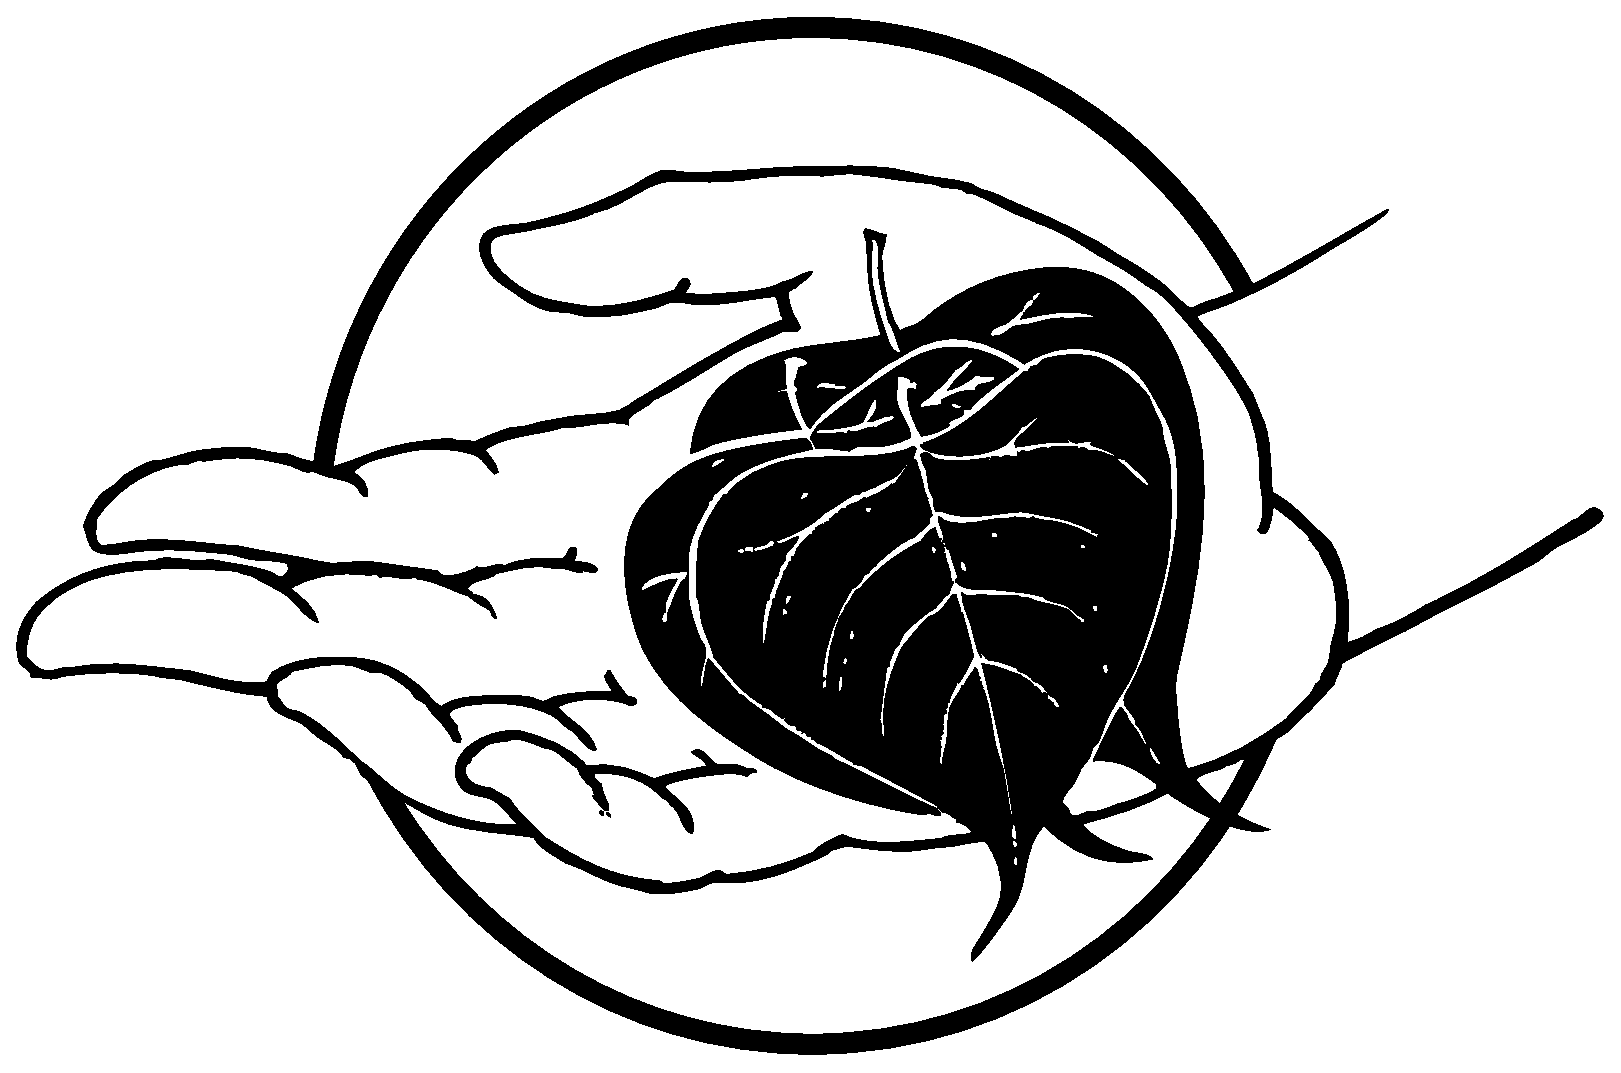
\includegraphics[width=1in]{abm_logo.eps}

\end{center}
\clearpage

\thispagestyle{empty}
{\footnotesize\raggedright
\vspace*{\stretch{1}}

\vspace{1em}
Abhayagiri Buddhist Monastery\\
16201 Tomki Road\\
Redwood Valley, California 95470\\
www.abhayagiri.org\\
707-485-1630

\vspace{1em}
\copyright{} 2014 Abhayagiri Buddhist Monastery

\vspace{1em}
This work is licensed under the Creative Commons
Attribution-NonCommercial-NoDerivatives 4.0 International License.

To view a copy of this license, visit
http://creativecommons.org/licenses/by-nc-nd/4.0/

\vspace{1em}

Interior design by Suhajjo Bhikkhu. Cover design by Sumi Shin.\\
Cover photos by Jonathan Payne. 


\vspace{1em}

We would like to acknowledge the support of the Kataññutā group of
Malaysia, Singapore, and Australia for bringing this book into full
production.

\vspace{1em}

\textit{sabbadānaṃ dhammadānaṃ jināti.}

The gift of Dhamma excels all gifts.
}

\clearpage


\vspace*{\stretch{1}}

This book is dedicated to our teachers and parents.

\vspace*{\stretch{2}}


\clearpage
\mbox{}\clearpage

\pagestyle{plain}
\tableofcontents*


%\thispagestyle{plain}
\clearpage

\thispagestyle{empty}
\mbox{} \clearpage

\chapter{Preface}

``Beginning our day \ldots{}''

These quintessential words are spoken by Luang Por Pasanno before he 
begins each of his morning reflections.

Five days a week, at Abhayagiri's morning meeting, work tasks are 
assigned to the residents and guests living in the monastery. Shortly 
thereafter, one of the senior monks offers a brief Dhamma reflection so 
that the residents and guests have something meaningful to recollect 
throughout their day.

These talks are given spontaneously and often address an event that is 
about to occur, a condition that is already present in the monastery, 
or a general teaching on Dhamma. The most common thread through all the 
reflections is that of practicality: distilling the most important 
teachings of the Buddha into pertinent and applicable practices. Though 
many different teachings are touched upon, the fundamental aim is to 
encourage the abandonment of the unwholesome, the cultivation of the 
wholesome, and the purification of the mind.

While several of these teachings may be read together at one time, 
readers might find it more useful to focus on a single reflection so 
they can easily recollect, contemplate, and make use of it throughout 
their day.

This book was made possible through the contributions of many people. 
Over ten years ago, Pamela Kirby initiated the project when she placed 
a recorder in front of one of the senior monks during a morning 
reflection and proposed that a book be written. Matthew Grad, Jeff 
Miller, Ila Lewis, Ray Peterson, and Laurent Palmatier were the main 
substantive editors of the material, enduring the long and difficult 
process of editing the transcripts into compact and well-written 
teachings. Ruby Grad and Pamela Kirby completed the copy editing. 
Shirley Johannesen compiled the glossary. David Burrowes, Dee Cope, 
Josh Himmelfarb, Evan Hirsch, Jeanie Daskais, Anagārika John 
Nishinaga, and members of the Lotus Volunteer Group: Wendy Parker and 
Viveka all helped with further refining of the text. Sumi Shin designed 
the cover. Jonathan Payne took the cover photos. Michael Smith tumbled 
the stones for the back cover.

For several years, Khemako Bhikkhu recorded the senior monks' 
reflections. Kovilo Bhikkhu and Pesalo Bhikkhu provided corrections on 
an early draft of the book. Suhajjo Bhikkhu generously dedicated a 
significant amount of time on the overall book design and typesetting 
of the text.

The Kataññutā group of Malaysia, Singapore, and Australia generously 
brought this book into full production.

Any errors that remain in these reflections are my own responsibility.

May these teachings bring insight into the nature of Dhamma and provide 
a pathway toward the development of true peace and contentment.

\vspace{1.2em}

\noindent Cunda Bhikkhu\\
Abhayagiri Monastery\\
Redwood Valley, California\\
May 15, 2014



\chapter*{Abbreviations}
\addcontentsline{toc}{chapter}{Abbreviations}

\begin{tabular}{l l}
DN & Dīgha Nikāya\\
MN & Majjhima Nikāya\\
SN & Saṃyutta Nikāya\\
AN & Aṅguttara Nikāya\\
Sn & Sutta Nipāta\\
Cp & Cariyāpiṭaka\\
Jā & Jātaka
\end{tabular}


\mainmatter

\mychapter{Directing Attention Skillfully}{Luang Por Pasanno}{April 
2005}

Learning how to meditate---how to develop the mind---is learning how to 
direct attention in a skillful way. Whatever we direct our attention 
toward becomes our reality. If we like, we can direct attention to all 
the chaos in the world or to the chaos of our own personal dramas. But 
we don't have to do that. We can instead direct our minds to 
contemplate our experiences as merely form, feeling, perception, mental 
formations, and consciousness. We can direct our attention in other 
skillful ways as well---toward objects that soothe the mind and conduce 
to peace and clarity. It's simple: We can incline the mind toward what 
is wholesome or what is troublesome. The choice we make is up to each 
one of us.

\mychaptertoc{Santuṭṭhi and the Meaning of Contentment}
{Santuṭṭhi and the\\Meaning of Contentment}
{Ajahn Amaro}{December 2008}

Contentment, or \emph{santuṭṭhi}, is often talked about in the 
context of material possessions, particularly in our reflections on the 
four requisites of robes, alms food, lodging, and medicine. It's the 
quality of being content with whatever is offered---the food that's 
presented to us each day, whatever shelter is available to us for one 
night, and whatever robes and medicine are accessible to us. That's an 
important aspect of contentment and a very grounding one---to have few 
material needs and few material possessions. There's a story about a 
man who found every one of his possessions torched in a large bonfire. 
All that remained were some ashes and the buckles from his boots. His 
response was, ``Well, good, now I don't have to bother with all that 
stuff anymore.'' This is what it means to be content with what we 
have---doing without if need be or living in our dwelling places with 
the thought that it is only a roof over our head for one night. This is 
our training.

It's also important to consider how santuṭṭhi permeates all aspects of
the path. It's not solely a matter of renunciation or not being moved by
desire, agitation, or fear in terms of material things or how we relate
to other people. Contentment is also the basis for concentration,
\emph{samādhi}---that quality of being content with this moment, this
breath, this footstep, this \mbox{feeling} in the knee, this sound in
the room, this quality of mood. To be content with just this moment is
of enormous importance in terms of samādhi, concentration.  And if
there's discontent---\emph{I have to become more concentrated, gain more
insight, be more comfortable, I have to, I have to}---then even though
we may be well intentioned, discontent continually creates a cause for
agitation and a lack of focus. As a result, samādhi is far away.

The quality of contentment can drift off in certain ways. It can turn 
into dullness or laziness or an urge to switch off, while at the same 
time we're thinking of ourselves as being content. Actually, we're 
simply steering the mind toward numbness, a non-feeling state or a 
feeling of wanting to get rid of, not bothering with. That's not 
contentment. Contentment isn't a quality of begrudging 
resignation---\emph{Oh well, I'm stuck with this mood, this particular 
problem or feeling. I'll just grit my teeth and bear it. I'll just wait 
for this to be over}---this is merely dullness, a nihilistic attitude. 
By contrast, when we are content there is a bright, radiant quality 
present. Contentment has a great lightness and clarity to it.

Contentment can also drift off in the opposite direction into 
complacency, self-satisfaction, being pleased with ourselves. \emph{I'm 
fine. I don't need to do anything with my mind. Everything is perfect.} 
That's taking it too far in the opposite direction. Contentment is a 
bright and energetic state, but it's also free from self view and 
self-centeredness. It's not colored by an I-me-mine attitude.

Santuṭṭhi is not only a basis for samādhi, but also for 
\emph{vipassanā}, insight. It's the ability to be content with seeing 
this feeling, this thought, this mood, or this memory as a pattern of 
nature. We're not buying into it, trying to read a story into it, or 
claiming it as self or other. Contentment allows us to leave things 
alone. A painful memory arises, does its thing, and ceases. An exciting 
fantasy arises, does its thing, and ceases. An important responsibility 
arises, does its thing, and ceases. That's it. This is a characteristic 
of contentment, we're able to leave things alone. The mental 
formations, the patterns of the world---we can let them be. It's not 
because we're switching off, we don't care, or we're resentfully 
resigned to some situation. Rather, it's a gentleness and presence of 
mind, a sense of the fullness of being. We're not needing to extract 
something from this thought, this feeling, this moment, or this 
experience.

Vipassanā is based on being able to attend simply to the process of an 
experience, rather than buying into its content. This requires 
restraint and in particular, sense restraint: not maneuvering to get 
more in the way of our requisites, not getting fussy and picky in terms 
of robes, food, shelter, or medicine. It's very basic. But the things 
we learn on such a basic, material level reach right to the core of our 
training, our spiritual practices, and our development of insight. It's 
the same with the quality of contentment---being at ease, tapping into 
the fullness of Dhamma, the completeness of Dhamma. It's always here 
because contentment is related to the quality of wholeness. It reflects 
the wholeness and the completeness of Dhamma. Nothing is missing, 
nothing needs to be added or taken away. Knowing this, we can be 
content with the way things are.

\mychapter{Breaking the Momentum}{Ajahn Yatiko}{April 2013}

We can take these next few minutes as a time to establish mindfulness 
and provide ourselves with a break. We can break the momentum of the 
mind, which so easily gets caught up in the process of becoming, 
especially when we have ongoing projects and duties to attend to. It 
can be so easy for the mind to obsess about unfinished tasks, keeping 
itself in a chaotic world. If we find ourselves stuck thinking about a 
project incessantly---trying to get it organized, straight, and 
complete---we can take a few minutes to stop.

If we can't stop that momentum, at least we can look to see if we have 
the mindfulness to recognize the flow of thoughts that come with it. We 
can pay careful attention to the mind that is creating time, a future, 
plans, and everything else and try to recognize and contemplate how 
this process is manifesting in our present moment experience. This is a 
very useful form of mindfulness, and we may find it to be a very 
valuable reflection when this momentum of becoming is such that we 
can't seem to stop it.

When we're not able to step outside of our usual patterns of thinking 
and instead find ourselves caught up in the flow of becoming or in the 
momentum of any kind of pattern---and we're identified with it---then 
it is similar to a form of craziness. Luang Por Chah famously once said 
that three seconds without mindfulness is like three seconds of 
madness. So even though we are wearing robes or are dedicated lay 
practitioners, we can still share the exact same chaotic mental state 
as 99 percent of the rest of the planet. In those instances we are 
caught up in the same momentum and are identified with it, not 
questioning it, and flowing on and on in the stream of becoming. So we 
need to use these opportunities and formal structures like meetings, 
\emph{pūjās}, Dhamma talks, and reflections to break that pattern. 
For you laypeople living outside of a monastery it is important to 
encourage yourselves to find environments where you can create a break 
in that flow of momentum. This can provide a space to establish 
mindfulness and allow you to reflect on your life skillfully. Otherwise 
life ends up being determined by patterns that have already been set in 
motion in the past---you're simply riding a wave. It may be difficult 
to find such places for yourselves, but it is important that you try.

These morning reflections are not just something to bear with and get 
over so we can get on to our jobs; they're here for us to use, to take 
up as subjects for contemplation. If we don't see very clearly how to 
use them in a skillful way, then we need to take that on as a 
reflection in and of itself. We can spend some time on the walking path 
or while we are sitting and ask ourselves, \emph{What is the morning 
reflection for? What is the right attitude to have when it is given?} 
Based on what arises out of this questioning, we can challenge 
ourselves further and ask, \emph{If this is the right attitude, is it 
something that I manage to have and cultivate, or have I allowed myself 
to have gotten into the habit of resisting formal structures?}

We are giving ourselves the space and time to pay attention to this 
flow of becoming and to use these reflections and wholesome structures 
to break the mind's unwholesome habits. By doing that we are slowing 
down the momentum of being relentlessly caught in cycles of rebirth and 
suffering. And when we have learned how to uproot this cycle, we come 
to a natural place of peace and freedom.

\mychaptertoc{Examining Uncomfortable Experiences}
{Examining\\Uncomfortable Experiences}
{Luang Por Pasanno}{June 2013}

Two days ago it was the anniversary of Ajahn Chah's birth. Many aspects 
of his life are well worth recalling and reflecting upon. Certainly one 
of them is the practical approach he used to teach and encourage us. He 
always emphasized the importance of reflecting on the Four Noble Truths 
and the experience of \emph{dukkha}---suffering, dis-ease, 
discontent---and the different ways we create dukkha within the heart. 
In this, Ajahn Chah embodied the quality of fearlessness---he had no 
fear when looking at the uncomfortable aspects of his own experience. 
By contrast, there is a tendency many of us have to try and run away 
from the uncomfortable experiences in our lives, to gloss them over or 
put some kind of spin on them. Instead, we need to look at them 
closely, without feeling intimidated.

I remember an example Ajahn Chah gave about this. He said, ``Sometimes 
you get a splinter in your foot. It's kind of small, and you don't feel 
it all the time, but every once in a while you step in a particular way 
that causes you to be irritated by it. So the thought arises, \emph{I 
really have to do something about this splinter.} Then you carry on and 
forget about it. But the irritation keeps returning until at one point 
you say to yourself, \emph{I really need to do something about this 
splinter now. It's not something I can put up with anymore.} Finally 
you dig it out. The experience of dukkha is the same.''

It's not as if we're experiencing dukkha all the time; for the most 
part, we live incredibly comfortable lives here. But there's this 
recurring sense of dis-ease, discontent, dissatisfaction. We need to 
make a strong determination to investigate it, understand it, resolve 
it, relinquish it, not shrink back from it, and really try to dig it 
out. We are trying to understand the nature of the human 
condition---the condition that keeps us cycling back to that feeling of 
dis-ease. It's a willingness to patiently put forth effort and to work 
with our experiences. This is an opportunity for us to learn how to do 
that in our daily lives and to learn how to do that in our formal 
meditation. It's possible to be carrying that investigation with us at 
all times.

\mychapter{Mindful of Right Effort}{Ajahn Karuṇadhammo}{November 2012}

Both on and off the cushion, we can examine how the activity of daily 
life is brought into the practice of Dhamma. In terms of the Noble 
Eightfold Path, many path factors are concerned with activities off the 
cushion. Developing \emph{samādhi} with sitting is just one part of 
the path. There is so much more that one needs to do to practice well 
and correctly. If we think of practice as that which is only on the 
cushion, then we are going to miss almost all the opportunities in our 
lives for deepening the practice.

We should keep in mind throughout the day not only right mindfulness 
but right effort. We do this by tapping into the awareness of wholesome 
or unwholesome states presently occurring in the mind.

It is important to check in with our current mind states, periodically 
investigating the mood of the mind so that appropriate attention is 
paid to what is happening. We can ask ourselves if we are dwelling in 
an unhelpful hindrance of aversion, craving, or some sense of 
impatience. Do we try to rush and finish an activity so that we can be 
by ourselves or do something that is more interesting than what we are 
involved in right now? If there is a hindrance present, notice what 
that state of mind feels like.

If they are unwholesome mind states or states that take us to a place 
that is going to lead to more stress and suffering for us or other 
people, then we can switch our attention and move into a state that 
will have a more positive effect on the mind. We don't need to 
reinforce negative states and allow them to drag us down.

Or conversely, is what we are experiencing wholesome or something that 
is helpful to support in the mind? We might, for example, enjoy being 
part of a work team and have positive experiences with other people. Or 
we might work alone and enjoy a wholesome activity that's good for the 
monastery. We can notice and reflect on these wholesome states of mind, 
encouraging, supporting, developing, and maintaining them.

Our goal throughout the day then, both on and off the cushion, is to 
check in every now and again as to the mood and quality of the mind. 
From there, we adjust as needed to bring about the wholesome and 
decrease the unwholesome.

\mychapter{A Balanced Perspective}{Luang Por Pasanno}{April 2013}

As most of us know, when bringing the practice into our daily lives, 
it's necessary to apply mindfulness. But it's also necessary to ensure 
that our mindfulness is operating under an appropriate and beneficial 
view or perspective. If we are mindful, but our view is misguided, then 
it's likely that we're mindfully following some sort of bias or 
obsession.

In order to keep on the right track, we need to question the views we 
superimpose on our experience. One way to expose those views is to 
notice the way we react to experience with comments and assumptions 
such as, \emph{This is really good---I like this. This is awful---I 
don't like this.} Reactions like those are habitual and need to be 
questioned.

When the mind assumes it likes an experience, it tends to block out the 
negative aspects in order to prop up the view, \emph{I like this.} So 
we need to deliberately bring up the negative side for examination, 
asking ourselves, \emph{What are the drawbacks? What are the pitfalls 
in this? How might I get hooked by it?} In the same way, when the mind 
experiences something it assumes is undesirable or challenging, we need 
to look at the situation from another perspective and ask ourselves, 
\emph{What's the beneficial side of this experience? What can I learn 
from it?}

When we examine our experience from both sides in this way, it makes us 
more flexible with regard to the views we hold. Instead of habitually 
seeing things as all black or white, we can open to a more balanced 
perspective from which we can see that experience is never just black 
or white---it's always a mixture. Without this balanced perspective, we 
tend to go through cycles of elation and depression, excitement and 
frustration and then wonder why that's happening. Well, in all 
likelihood, it's happening because we've attached ourselves to some 
sort of all-or-nothing view.

Ajahn Chah encouraged us to question our views of experience by having 
us ask ourselves, \emph{Is this for sure? Is this really what's 
happening?} By doing that, we can better adapt to whatever circumstance 
we find ourselves in, because we're no longer preoccupied with trying 
desperately to force circumstances to be the way we like them. And it 
becomes easier to be mindful and present with experience as it unfolds.

So whether we're attending to our duties, engaged in some kind of 
interaction, or alone, we need to question the habitual views and 
reactions that come up for us. Otherwise, those views and reactions 
will toss us around like a feather in the wind---wherever the wind 
blows, that's where we'll land.

\mychapter{Don't Fill Up the Void}{Ajahn Jotipālo}{July 2012}

Why did you come to Abhayagiri? What brought you here? Simply bring 
that inquiry into your mind.

After traveling for the last month and being fairly busy, I returned to 
Abhayagiri a few days ago. I've tended to go back to my \emph{kuṭi} 
in the afternoons, and it's been really quiet. There have been no 
expectations or demands on me. I've noticed in the past, after a period 
of busyness, when I go back to my kuṭi for some quiet time, there is 
a feeling of melancholy that comes up and a feeling that I should be 
doing something. I've been looking at that for the last two days, going 
back to my kuṭi and sitting there with that feeling. I'm not trying 
to label it---anxiety, depression, or whatever else the mind wants to 
call it. I'm just looking at it as a physical sensation and seeing how 
the mind is reacting to it, how the mind is trying to figure out what 
it is, and why it's there. When I feel this way my tendency and desire 
is to say to myself, \emph{I should go do something to help the 
monastery or read a book or do walking meditation \ldots{}} There is 
this low-grade desire in me to avoid feeling this melancholy. I don't 
\emph{want} to feel it. Even something as wholesome as reading or 
studying, if the intention behind that is to avoid feeling something, 
then it's good to investigate that.

For at least a period of our afternoon, when we have solitude, I think
it is good to set aside some time to do nothing in particular. Don't
think of it as trying to meditate or trying to \mbox{focus} on the mind,
just sit there and be willing to feel what you're feeling. See what
happens.  See if it's aversion or pleasure. To me, this really gets back
to that first question, \emph{What brought me here?} We are often trying
to fill up the void we feel with activities, planning, or whatever,
merely because we don't want to feel the discomfort of that void, or of
any other unwanted emotion. When we do this, we are not honoring the
wholesome intentions that brought us here. So instead, when we find
ourselves avoiding our experience, we can take the time to be quiet and
be willing to feel what we are feeling.

\mychapter{Stopping}{Luang Por Pasanno}{July 2005}

The other night Ajahn Sucitto gave a Dhamma talk about the type of 
kamma that leads to the end of kamma, and one type of kamma he spoke 
about was stopping. The importance of stopping is often overlooked. We 
get so caught up in doing, becoming, activity, and engagement that we 
don't attend to stopping---it's a neglected aspect of our practice. 
This isn't about sitting around doing nothing, because that's a form of 
doing as well. It's about stopping habits of greed, irritation, and 
confusion. It's about stepping back and ceasing.

Throughout the day, during work periods and in meditation, we can 
reflect on how much the mind gets swept up in activity and in 
identifying with that activity. We can also reflect on how this 
tendency moves the mind toward restlessness and agitation from which we 
lose our center: one little push, the ball starts rolling, and pretty 
soon we've worked ourselves into a state of anger and conflict. With 
desire, it often starts with the merest sort of interest, which then 
becomes liking, fascination \ldots{} and then we begin to lose control. 
We don't know how to stop this momentum of desire because we're not 
used to stopping. It's also helpful to reflect on the occasions when we 
do happen to stop. We might ask ourselves, \emph{Does stopping mean I 
can't function? Or is it more that when I stop and stand in awareness, 
I accomplish things more skillfully than when the mind is swept up by 
moods and thoughts?}

These reflections help motivate us to learn how to stop the mind, how 
to stop the flow of proliferating thoughts and moods that draw us into 
attraction or aversion. If we learn how to stop the mind and exercise 
that skill frequently, then even in challenging circumstances, we will 
be able to bring things to a point of stillness inside and return to a 
clear center of awareness.

So how do we learn to stop? When we feel the mind moving and 
proliferating, how do we stop and come back to a place of awareness 
where we can attend to what the mind is doing and is intending to do? 
To begin, we can recognize when the mind has stopped on its own. Then 
we can observe what stopping itself feels like---the actual 
\emph{experience} of ceasing to engage with mental activity and mental 
impulses. Once we become familiar with how stopping feels, we'll know 
when our conscious efforts to cultivate stopping are on the right 
track. It's helpful to make this cultivation into a regular 
exercise---something to frequently work, play, and experiment with.

Certainly we need to engage in activities and attend to our duties and 
responsibilities, but we can bring an attitude of stopping into the 
midst of this activity, whether it's the stopping of obsession, worry, 
fear, competition, aversion, or whatever. We may try to replace such 
unwelcome mind states with something we feel is more appropriate for 
``good Buddhists,'' but trying to replace one thing with another is yet 
another form of doing. Instead, if we simply attend to stopping, we 
learn to trust in fundamental clarity and wisdom.

\mychapter{Loving-Kindness for Ourselves}{Ajahn Yatiko}{December 2012}

When we do \emph{mettā} meditation, loving-kindness meditation, it's 
often good to start with ourselves. But when doing that, it is 
important that we not put ourselves under our thumbs---making demands 
about who we are and what we should be. When this happens, it's as if 
we're looking at the mind the way judgmental parents look at their 
child, power tripping and demanding that the child behave in a 
particular way. \emph{I'm going to tell this kid what to do, and he's 
going to do what I say!} There can be no joy in approaching the mind 
with the assumption that it will toe the line if we force it to do so. 
Joy has to be unfettered with a sense of real freedom.

When we practice loving-kindness meditation, we turn our awareness and 
consciousness toward our sense of being, our sense of existence, and we 
give ourselves the space and freedom to be exactly as we are. There are 
no demands placed on us---not on our physical bodies or on our 
personalities. All of our expectations are irrelevant; they are a 
fiction. We give ourselves freedom to be what we are, and from that 
freedom we wish for ourselves, \emph{May I be happy.}

For many of us, there can sometimes be a sense or even an insight that 
our \emph{modus operandi} is not to be happy. For me, when I look at my 
own behavior, it doesn't always feel like it's coming from a wish for 
happiness. It can be like that for all of us, so we cultivate mettā as 
an antidote. We turn our awareness toward mettā, and eventually we may 
have a deeper insight: \emph{Actually, I really do want to be happy, 
and my heart genuinely wants that freedom.} The greatest freedom we can 
experience is not the freedom of letting ourselves do what we want out 
in the world. The Buddha says that freedom in its highest form is 
freedom from affliction; it's not from the gratification of the senses. 
It's simply the experience of sitting here with very little suffering 
occurring for us; we're not making problems out of our experience.

When we have loving-kindness for ourselves, we want to imbibe the sense 
that we are what we are, and we don't need to make a problem out of any 
of it. We want to tune into the sense that generating loving-kindness 
for ourselves \emph{is} what our hearts want---we want to be happy and 
free from suffering. We genuinely want to care for ourselves. It's 
almost insane how we don't act in our own best interests, how we forget 
that this is actually what we need to be doing. So we need to make a 
conscious effort to value our own well-being and to recognize the 
heartfelt wish for our own happiness.

When doing loving-kindness meditation, we give ourselves space, 
freedom, and acceptance. We express ourselves from a nonjudgmental 
attitude, \emph{I am what I am, and however I am, that's okay.} We 
bring up the wish, \emph{May I be happy.} Then we relax into that space 
and see what happens.

\mychapter{To See the True Nature of Things}{Luang Por 
Pasanno}{December 2004}

Without clearly understanding the processes of our minds, we create all 
kinds of problems. We are dragged about by emotional states. For there 
to be personal and global peace, these states need to be understood. 
The ways of the mind need to be seen clearly. This is the function and 
value of Dhamma.

When we are feeling enthusiastic, we can easily give ourselves to the 
practice. But it can also happen that, at times, we feel completely 
disillusioned, even to the extent that we forget the original 
confidence and faith we had. But that's natural. It's like swimming a 
long way. We become tired. There's no need to panic, we can simply be 
still for a while. Then when we have regained strength, we continue. 
When we understand in accordance with nature, we understand these 
states will change. Despair, if that is what has arisen, will pass. We 
keep practicing. By observing our minds and seeing how our attitudes 
are continually changing, we more clearly understand that impermanence 
is natural.

Isn't cultivating Dhamma as important as breathing? If we stop 
breathing, then we die. If we are not established in the right 
understanding of truth---the truth of the way things are---then also we 
die. We lose touch with what is truly good. If we are lacking the 
richness of truth in our hearts, then when we die and they cremate us, 
our lives will be worth no more than the handful of ashes we 
produce---and that's not much! We must investigate how to live in a way 
that truly accords with what the Buddha taught. Then we can live in 
harmony without conflicts, difficulties, and problems. \emph{Sīla}, 
morality, is that which shows us the Buddha's Middle Way. It points to 
the avoidance of the extremes of pleasure and pain; it means knowing 
the right amount. When we live in the Middle Way regarding actions of 
body and speech, then we don't cause offense to others; we do what is 
appropriate for human beings. The practice of formal meditation is to 
train our minds and hearts to stay in the Middle Way.

Many people who meditate try to force their minds to be as they want 
them to be. They sit there arguing with their thoughts. If their 
attention wanders, they forcibly bring it back to the breath. Too much 
forcing is not the Middle Way. The Middle Way is the ease that arises 
naturally in the mind when there is right effort, right intention, and 
right awareness. When the practice is right and there is ease of mind, 
we can simply watch the different states that arise and consider their 
nature. We don't need to argue with anything. Arguing only causes 
restlessness. Whatever emotion arises is within the domain of our 
awareness, and we simply watch. Whether it's joyful or the absolute 
opposite, each experience is within the boundaries of our awareness. We 
just sit, watch, recognize, and contemplate them all. They will 
naturally cease. Why do they cease? Because that is their nature. It is 
this realization of the true nature of change that strengthens and 
stills the mind. With such insight there is tranquility and peace.

What we call ``me'' is merely a convention. We are born without names, 
then somebody gives us a name. After being called this name for a 
while, we start to think that a thing called ``me and mine'' actually 
exists. Then we feel we have to spend our whole lives looking after it. 
The wisdom of the Buddha knows how to let go of this ``me,'' this 
``self,'' and all that pertains to it---possessions, attitudes, views, 
and opinions. This means letting go of the conditions that make 
suffering arise, and that requires taking the opportunity to see the 
true nature of things.

\mychapter{Recollecting Our Goodness}{Ajahn Amaro}{December 2008}

When we're engaged in a lot of activity, we can become so focused on 
the details of what we're doing that we forget there's an element of 
generosity and goodness in our actions. When Ajahn Sumedho was a young 
monk, Luang Por Chah recommended that he recollect his good qualities. 
Ajahn Sumedho couldn't understand what Luang Por was talking about 
because his mind was quite busy and filled up with negative thoughts 
and emotional habits. He thought of himself as basically a selfish, 
nasty, horrible person, and an embarrassment to the robes.

Luang Por Chah told him, ``If you're such a bad person and really evil, 
you wouldn't want to live with Buddhist monks. We would be the last 
people you would want to spend time with. If you're so off the mark and 
if your mind is so given to unwholesomeness, you wouldn't want to be 
around people who are honest, refrain from stealing, refrain from 
consuming intoxicants, people who don't behave in unruly ways. The last 
thing you'd want to do is be around virtuous people.'' When Luang Por 
said this to him, he was quite startled by it. He thought to himself, 
\emph{You know that's true. I can easily forget that I'm living in a 
Buddhist monastery with Buddhist monks. There must be some reason why 
I'm doing this.}

We can become quite focused on our faults, wrongdoings, and the things 
we said that were less than generous, friendly, helpful, or patient. 
Even after someone has asked us for advice, what we think about later 
is how much better it would have been to have said this or that. 
\emph{Oh, I really didn't get that right.} The attention goes to all 
our shortcomings, failures, and weaknesses, and we obsess on those 
qualities.

That's how it was for Ajahn Sumedho. So when Luang Por Chah suggested, 
``Why don't you recollect all of your good qualities?'' there was no 
pigeonhole for him to put them in. At that time any good quality he 
had, he saw as inflated, egotistical, proud, or conceited. But Luang 
Por said, ``No. This is \emph{cāgānussati}, recollecting your 
goodness, recollecting your own generosity. It's a completely normal 
concept.'' Now, since we've had the good fortune to hear Laung Por 
Chah's advice to Ajahn Sumedho, it would behoove us to put that advice 
into practice for ourselves.

One way for us to do that is to recollect all the good effort we're 
making in looking after the kitchen, providing food, looking after the 
construction projects, the \emph{kuṭis}, the buildings, or the 
micro-hydro project we're setting up. These are acts of generosity and 
kindness, of putting forth effort and putting forth our time to help 
other people. Many people have helped with the construction of the 
kuṭi down by the Bhikkhu Commons. Of those people, how many are 
actually going to live in it? Probably a very small proportion. The 
effort that we make is not simply in the single task we do, but also in 
the wholesomeness and goodness it supports---the \emph{kusala kamma} it 
supports. By providing this dwelling, this food, these Dhamma talks, we 
bring enormous blessings into our lives.

Take Tan Ṭhitapañño, for instance. He's wrestling with the 
intricacies of the Expression Engine software and the obstructive 
passwords that won't let him use the program. When doing such hard 
work, it can be easy to forget about the fact that there are people all 
over the planet who delight in what this work accomplishes, \emph{Oh 
look, a new Dhamma talk on the Abhayagiri website. How marvelous! This 
is fantastic!} This isn't simply about trying to cheer ourselves up or 
look on the bright side. This really is the bright side. Earlier in the 
year a fellow came to Abhayagiri from Liverpool, England. He was so 
happy to be here. He didn't even stay for a full day. He happened to be 
in the country on holiday and took a chance to visit us. He said, ``We 
have this little meditation group in Liverpool, and we listen to 
Abhayagiri talks all the time. It's so great to be here.'' He was 
bubbling with happiness. We can forget that our lives are connected 
with little groups of people like that all over the planet. In our 
small efforts to keep the bodies fed, to keep the shelters workable, to 
provide Dhamma talks on the website, to offer publications, to pay the 
bills---every little piece is bringing goodness into the world. That's 
kusala kamma, wholesome action.

It's not indulgence, egotism, or pride to be reflecting on that 
goodness. The Buddha himself encourages cāgānussati, recollecting our 
generosity, because that brightens and brings joy to the mind. We can 
take some time to recollect all the efforts that we're making on the 
practical front as well as with the formal meditation practice. The 
word \emph{anumodanā} means rejoicing in the goodness that has been 
done. The cynical mind says, \emph{Yeah, well, that's one thing. But 
I've really got some serious problems. Basically I'm just a defiled 
mess. I really am!} We need to listen to that voice with compassion, 
but at the same time, we don't want to let it run our lives. So we 
listen and then gently park it to one side. We can reflect, \emph{Even 
if I'm filled with utterly ghastly defilements, still there are things 
I've done that have helped people. That's an undeniable fact. There's 
some goodness or brightness that I've brought into the lives of others. 
My effort to be a little bit more patient has benefited other beings. 
How wonderful!} By letting that brightness inform our lives, we can be 
encouraged and gladdened by it.

\mychapter{Where Did That Self Go?}{Ajahn Karuṇadhammo}{December 2013}

This morning we chanted the recollection of the ``Thirty-Two Parts of 
the Body,'' as well as the Anattalakkhaṇa Sutta, which mentions 
thoughts, perceptions, and feelings. They can both be used to reflect 
on aspects of not-self.

The ``Thirty-Two Parts of the Body'' is a reflection that can be 
utilized to reduce sensual desire when there is a strong attachment to 
the human body as an object of attraction. We can also bring this 
reflection up as a way of dividing up what we usually consider a unit, 
a whole, something to attach a sense of self to. Oftentimes we identify 
with this body as either ``me'' or ``mine,'' as something I possess or 
something that is actually who I am. The ``Thirty-Two Parts of the 
Body'' contemplation helps us tease the body apart so that we can 
reflect on how this body is just a collection of parts, any one of 
which we would be hard-pressed to say is who I am or ``me.'' We can ask 
ourselves, \emph{What would happen if I lost an arm or a leg or had a 
body part that had to be taken out because of disease? If I take 
something away from this body then what is left is different. So is 
this body any less me than it was before? Or is it a different me? Or 
perhaps it is not me at all?} That is one way that we can reflect on 
the ``Thirty-Two Parts of the Body.''

Our friend Iris's cancer has moved to her brain. Although she is having 
treatment, her perceptual world seems to have been altered in some 
ways. She perceives the world around her differently than she normally 
did or how we normally do. When we look at things in a different way or 
see different aspects or angles of physical and mental phenomena, it 
can help us see how much stock we put into the continuity of the 
perceptual realm. As the Anattalakkhaṇa Sutta suggests, we can see 
how we attach to our perceptions a sense of ``me,'' ``myself,'' and 
``who I am.'' This continuity of thoughts, perceptions, and feelings 
weaves a web of self and sometimes gets changed or altered or 
diminished. \emph{Where did that ``me'' go to? Where did that self go? 
Is it a different one? Is it the same one but looked at from a 
different angle? Or is it possibly just another perception that I have 
weaved together to give a sense of security and stability?}

It is good to reflect on the change and instability of what we normally 
call ``me'' or ``mine,'' both in the body and in the mind. We can take 
this up as a contemplation and examination, and ask ourselves, \emph{Am 
I really any of these?}

\mychapter{Not Reaching for the Stars}{Luang Por Pasanno}{July 2013}

In an ideal world, a summer day like this would be 80 degrees with a 
gentle breeze. In reality, it's 108 degrees, and the air is not moving 
at all. How do we handle the contrast between what is ideal and what is 
real? We can moan and whinge or retreat into fantasy and desire, but 
from the Buddha's perspective, it's always about establishing a sense 
of clarity and equanimity within the reality of the present moment.

With something like the weather, it's fairly easy for us to see our 
unrealistic hopes clearly and accept them for what they are. But in 
other areas, it's more difficult. For instance, living as we do in a 
spiritual community, we may hold to a utopian notion that everyone here 
should be mindful, peaceful, contented, and harmonious. And it's 
true---we should be. But we can keep in mind that this ``should'' is 
based on an ideal. The reality is oftentimes quite different. So it's 
necessary to learn how to navigate those times when we, or others, 
aren't living up to the elevated principles that we hold. To do that, 
we can reflect on whether it's realistic to expect everybody to live up 
to our lofty notions simply because these notions are what we would 
like or prefer. We can reflect on how well we personally adapt and 
respond to the realities of our existence and see that it is often 
difficult to live up to our \emph{own} ideas of perfection.

This doesn't mean we should throw out all the ideals we have and tell
ourselves to forget it. Holding to wholesome \mbox{ideals} can be a
skillful thing to do. But we need to be very cautious of measuring
ourselves against those high values all the time. Doing that exacerbates
dissatisfaction, discontent, and a sense of suffering.

In former times, navigation at sea depended on frequently checking the 
stars with a sextant to set and maintain a realistic course of 
direction. It wasn't about trying to reach the stars! In a similar way, 
as practitioners we merely need to set ourselves on a wholesome, 
skillful course; we don't need to constantly frustrate ourselves or 
others by trying to comply with unrealistic notions of perfection. 
Usually our ideals---even wholesome ones---are filled with wishful 
thinking and fantasy. So it's important to ground our elevated 
standards in reality. By doing that, we can find a realistic course of 
action that supports our living skillfully. Applying the Dhamma in our 
day-to-day lives, we can learn to live with each other and with 
ourselves in a beneficial, wholesome way.

\mychapter{Determined to Suffer}{Ajahn Yatiko}{July 2012}

We suffer because we are not seeing things with the right perspective.

We're here in this monastery by choice, and all the work is done on a 
voluntary basis. It's a good place. Within this sort of environment, 
there is no need to suffer. Things are the way they are. But through it 
all, we still seem to have an insatiable need to suffer. We are 
absolutely determined to not let go or soften our perspective. It's as 
if we'd rather suffer than grow. The problem is we don't realize that 
suffering is going to grow and grow and grow. Eventually we are going 
to have to let go of all the situations that cause suffering, such as 
loss, physical pain, uncertainty, or whatever it is we don't like. It's 
just the way it is.

The fact that we experience a particular object as something we don't
like is because of the way we structure our values and priorities
\emph{within}. None of what we experience from the outside---be it
community, people, activities, or responsibilities---has an objective,
factual existence. It's something that we experience through our
internal senses. We give meaning to things and, based on the meaning we
give, we attach to this and hate that. We create an entire world out of
what we experience, and we end up \emph{living} in that world. The
world, as we know it, isn't actually out there; it's in our heads.
\mbox{Understanding} this helps us to see that our suffering is coming
from our own actions, views, and decisions and not from the outside.

This sort of reflection is empowering because it puts us in control. 
There's really nothing and no one else we can blame. This truth is 
especially apparent when we live in a monastery like this. It's good 
enough to carry out our practice. Perhaps it's not so apparent for 
people immersed in a cultural setting---local or global---where ethics 
are not a priority and introspection is not encouraged or valued. In 
that situation, it's easier to convince ourselves that our choices and 
actions are taking place in an external world.

But that perspective doesn't hold sway in the environment we have here. 
So we can surrender to the situation, the routine, the principles, and 
the practices of the monastery and learn to let go. Through that 
quality of surrender, the heart starts to feel a sense of release. We 
start to gain a sense of confidence as to what the spiritual life is 
really about and what's important in our life.

\mychapter{Containing the Chicken}{Luang Por Pasanno}{August 2012}

The theme we used for Upāsikā Day yesterday was brightening the mind 
and focusing on the ten \emph{anussati}---the ten recollections: 
Buddha, Dhamma, Saṅgha, virtue, generosity, celestial beings, 
mindfulness of the body, mindfulness of death, mindfulness of 
breathing, and Nibbāna---peace. Several people expressed their 
appreciation for being taught about the ten recollections in that it 
gave them more freedom and flexibility to work with the mind.

Meditation can often become mechanical or method oriented, or focus 
solely on concentration and trying to get the mind to stop thinking. 
Sometimes when we practice like this, there tends to be a lot of effort 
expended, and this can agitate the mind. However, the Buddha taught 
ways of using the thought process so that it supports the cultivation 
of wholesome and bright states of mind. Thinking in this way naturally 
leads the mind to settle down. The mind naturally settles when it feels 
good, when there's a quality of well-being. We encourage this by 
bringing to mind directed thought and attention and evaluating the 
result of that. When we do this, there can be a continuity of wholesome 
and skillful thoughts, and the mind can become settled and clear.

Ajahn Chah said that meditation is like containing a chicken. In a 
village, when a person has a chicken and is concerned that it's going 
to run off, he gets a loosely-woven large bamboo basket and plunks it 
over the chicken. Rice can be put in the basket, and the chicken stays 
in the container. One doesn't have to tie the chicken down or keep it 
from taking a step anywhere. Having a container for the chicken is 
sufficient. In the same way, when the mind is imbued with a sphere of 
awareness and intention, and attention is being directed on a wholesome 
theme, then the mind will stay within that container. It doesn't mean 
that it's forced to stay there, but it's content within that sphere. 
These recollections are a skillful means of directing attention, 
bringing wholesome recollections to the mind so it will settle within 
that container.

Both in our formal meditation practice and throughout the day we can 
bring to mind and recollect the Buddha, the Dhamma, the Saṅgha, 
virtue, generosity, celestial beings, the body, death, the breath, and 
Nibbāna---peace. Another helpful theme that is not on this list is the 
quality of \emph{saṃvega}, spiritual urgency or a chastening of 
worldly tendencies. This can help remind us of death and the 
limitations of the body. A complementary theme for saṃvega is to set 
up the intention to put forth effort, to realize what the Buddha taught 
and the example that he set. Another important quality that comes to 
mind is \emph{pasāda}, which is a sense of serene confidence and 
clarity of well-being; it has a joyful sense to it.

We want to encourage these ten recollections in our practice as well as 
these other skillful qualities so that we create a wholesome foundation 
for the mind. We have a lot of space to experiment and work with these 
themes. As we get to know them, we can see what works and what helps 
the mind direct itself toward the Dhamma.

\mychapter{Skills for Letting Go}{Ajahn Ñāṇiko}{December 2013}

In our practice we are normally working with the core defilements of 
greed, anger, and delusion. Often when these defilements arise, the way 
we deal with them is through restraint. When we restrain the 
defilements it feels different than actually letting them go. With 
restraint, we continue to experience the defilement; it's an 
undercurrent in the mind. By contrast, when we genuinely let something 
go, there is a feeling of being completely refreshed and replenished. 
There can be an experience in both the body and the mind of being 
filled with a clear, cool, pure substance. Restraint is important as 
well, however. When there is irritation or anger in the mind, or a 
nagging desire that won't go away, we can first use restraint as an 
antidote by applying, for example, \emph{mettā} or \emph{asubha} 
practices. The mind will then loosen its grip on these defilements and 
let go.

Sometimes we may think it's impossible for the mind to let go, but it 
is important that we not think this way. The mind will let go in its 
own time according to its conditioning and its kamma. In particular, 
letting go depends on the kamma of our skillful effort in the practice. 
We don't need to figure out when the mind will let go, we just keep 
practicing. Walking, standing, sitting, or lying down, we keep the 
Dhamma teachings in mind, moving forward with faith that true letting 
go is possible. It is not helpful to tell ourselves, \emph{I don't have 
enough pāramī to let go.} Letting go is a skill. Everyone has to put 
forth effort, especially when we are just beginning.

Learning how to fail is another important part of the letting-go 
practice. About a month ago I was trying to fix an old planer. It was 
difficult to get the blade removed. I was in the shop with Doug, and I 
told him, ``I'm prepared to fail at this, but I'll give it a try.'' 
There was one screw with a stripped head, and after awhile I finally 
managed to remove it. I was so excited when I took it out that I forgot 
to take out the other screw that didn't have any problems. I started 
prying the blade out and ended up breaking the planer entirely. 
Afterward I reviewed my mind, and I thought, \emph{I told Doug that I 
was prepared to fail at this, but actually I wasn't prepared to fail at 
all.} I spent the next three days mired in \emph{dukkha}, full of 
reproach about my foolish mistake. It took quite a while to let that 
one go. So it's important to learn how to fail without taking it 
personally. After all, taking things personally is the very thing we're 
learning to let go of.

\mychapter{Faith Develops Energy and Wisdom}{Luang Por Pasanno}{June 
2012}

Faith is an essential part of our practice, and it's not something that 
magically appears on its own. Rather, the arising of faith takes 
effort. We need to direct our attention toward it, to frequently 
reflect on the arising of faith as a real possibility for us.

As Westerners, most of us are not on familiar ground when we reflect on 
faith. But it is an important quality for balancing the different 
aspects of our practice. In particular, faith comes first among the 
five spiritual faculties. It is used to balance wisdom, the fifth 
faculty, and to support energy and effort---the second faculty. How 
does that work? Wisdom arises from investigative analysis, and, without 
faith, investigative analysis becomes dry, and we tend to lose energy. 
The qualities of faith include confidence and devotion, both of which 
naturally result in increased energy and effort. Energy and effort need 
to be nourished, and faith is an important part of that nourishment.

The opposite is true as well: When the wisdom faculty is lacking in 
faith, it often leads to cleverness and a superficially critical way of 
evaluating things. Without faith, wisdom can increase our negativity, 
which in turn can reduce our own energy and the energy of the people we 
engage with.

For many reasons, it is important to turn our attention toward faith, 
to reflect on it, so we can recognize faith as an essential part of our 
practice.

\mychaptertoc{Mindfulness of Death, Appreciation for Life}
{Mindfulness of Death,\\Appreciation for Life}
{Ajahn Karuṇadhammo}{May 2013}

Luang Por Pasanno mentioned that Debbie's mother is going to be signing 
into the palliative and hospice care programs because her condition is 
deteriorating. I would think Debbie has been practicing with death 
contemplation as this is happening, particularly after she lost her 
sister-in-law a few months ago. The Buddha encouraged us to reflect 
daily and remind ourselves that death can come at any time. It's easy 
to externalize, \emph{It's happening to somebody else, not me.} But at 
some point, it won't be somebody else, it will be us, and it would be 
nice to think that we are ready for it when it comes. This isn't meant 
to be a morbid reflection, but more an encouragement to contemplate 
death, bringing us closer to the reality of it and to encourage a sense 
of heedfulness and urgency in the practice.

It's so easy to get lost in the tasks of the day, particularly as we are
about to launch into a work period. I would imagine that a significant
number of people right now are thinking about the tasks they need to do.
I find myself doing that sometimes as well. But we can pull back a bit
and remind ourselves, \emph{Hold on a second, life is precious. I don't
know when or how I'm going to die. If death occurred for me right now,
would I be ready for it? Would there be remorse? Are there things that I
have done or left undone that I would regret if I died today?} We can
take a few moments to \mbox{contemplate} the potential immediacy of
death and see what this might bring up for us.  Contemplating death in
this way allows us to clarify what is precious in our lives which frees
us from the tendency to get lost in the details. This in turn helps us
focus on what our priorities are. So instead of death contemplation
producing a negative feeling such as fear or bewilderment, we can be
moved to a sense of lightness and release as we focus on what is most
important to us. A life well lived, focused on what is most meaningful
for us, has the greater potential to be a life free of regret and
remorse.

Death is a present-moment experience; it's not in the future. When the 
moment of death arrives, it will be just that moment---everything 
before that moment of death is still life, with all of its projections, 
worries, and fears, including the fear of that approaching death. But 
when death actually occurs, it is just one brief moment. So at the 
moment of death, death is now. Before that moment, it is just a 
projection. With contemplation of death we become more familiar with 
this inevitable ending so that when it finally comes, we are prepared 
for it, neither afraid of it or confused with this very ordinary 
present-moment experience.

If we keep that in mind then we do not really have any other option 
than to contemplate what's going on for us right here and right now. 
It's the only place we are going to be ready when it's time for the 
body to move on, for the elements to dissolve. For most of us, one of 
the best ways to do this is by using mindfulness of the body. We can 
notice the position of the body, the posture of the body---standing, 
walking, sitting, and lying down. This is the most basic contemplation 
of the body, and we can maintain it when we are doing just about 
anything---constantly coming back and asking ourselves, \emph{What is 
the posture of the body? What is the disposition of the body? If it's 
moving, how is it moving through space?} We can know what's happening 
with the arms, the legs, the head, the torso, and be present with the 
body. We can also incorporate the mood of the mind, \emph{What's the 
mood like right here and right now?} If we keep on attending to right 
here and right now as we go through our daily activities, then when it 
comes time for death to greet us, we will be ready right there and 
right then to be aware of the event as it happens. Bringing mindfulness 
right here and right now and reminding ourselves of the preciousness of 
this human life is a great way of reducing fear and anxiety and 
establishing a sense of purpose along the path.

\mychapter{Truthfulness in Speech}{Ajahn Yatiko}{June 2013}

One way we are generous with each other here at the monastery is in the 
realm of truthful speech---an attribute that is essential in one who is 
walking the Buddha's path. The notion of truthful speech is deep and 
profound. It doesn't simply mean saying things that are truthful; it 
also implies expressing ourselves honestly---being able to clearly 
communicate with others, even when there's a thorny issue at hand.

Sometimes our attempts at communicating can be hopelessly indirect, 
which is not helpful. For example, if we feel somebody is being unkind 
to us, rather than letting them know, we might instead ostentatiously 
increase our ``kindness'' around them, hoping they'll get the message 
and change. This rarely works and can sometimes be seen as 
passive-aggressive. So it's important to establish genuinely truthful 
speech to directly express our needs to others, at the appropriate 
time, so they can hear and understand us. This takes practice, but it's 
very much a part of the path.

More generally, it is also important to act with a generous heart, no 
matter what we're doing. This requires an attitude of taking 
responsibility, recognizing that all institutions---families, 
monasteries, and communities of all kinds---require people to take 
responsibility, to open their eyes, and to see what needs to be done to 
help others.

Sometimes when we see somebody in need, physically or emotionally, we 
may think to ourselves, \emph{Well, this is a big place, and someone 
else will take care of the situation.} When we think in this way, it's 
as if we are placing an invisible force field around those who are in 
need so we can't see them or their problems. Ajahn Amaro has 
colloquially referred to this phenomenon as if people are approaching 
the world with an ``SEP field''---a somebody-else's-problem field. In a 
large community like this, it can be easy to take the SEP field 
approach and ignore the problems of visitors or those we live with. But 
we mustn't let these people slip through the cracks or fall by the 
wayside. This requires a resolve to help those in need as best we can 
and not just for their sake. Our holding to such a resolve will help 
improve the overall sense of well-being, functionality, coherence, 
harmony, and brightness in the community we're living in.

\mychapter{An Auspicious Day of Blessings}{Luang Por Pasanno}{July 2012}

Today is Friday the 13th, and by tradition some people believe that 
it's an unlucky day. Many people have different ideas of why Friday the 
13th became known as an unlucky day. In the Thai tradition and the 
Asian tradition in general, there are lucky days, unlucky days, 
auspicious and inauspicious times. Ajahn Chah used to say that whatever 
day we are doing something wholesome, that is an auspicious day. He 
also said there is no such thing as a day in and of itself that is 
inauspicious or unlucky. We are completely dependent on gathering our 
own resources into doing something that is skillful, beneficial, and 
wholesome. So the opportunity for doing that which is wholesome is in 
itself what makes it a blessing in the world. The Pāli word 
\emph{mahāmaṅgala} means the highest blessings. The Mahāmaṅgala 
Sutta encourages the cultivation of that which is skillful: association 
with good people and developing inner virtues that are beneficial to 
both ourselves and others (Sn 2.4). When we cultivate these virtues, we 
create the blessings of a skillful life, sharing those blessings with 
the people we're living with and the people we come into contact with. 
That is how we bring great blessings into the world.

\mychapter{Non-Contention Is Full Awareness}{Ajahn Amaro}{December 2002}

Under the Bodhi tree the Buddha's response to death---in the form of 
Māra's threats, cajolings, temptations, and attempts to cause 
doubts---was not life-affirmation, going into a deep state of 
concentration to evade Māra, blasting him with a \emph{vajra} bolt, 
trying to be reasonable and negotiate on Māra's terms, or trying to 
justify himself. Instead, the Buddha's response was a fearless 
wakefulness. Almost invariably, throughout the accounts of the Buddha's 
meetings with Māra, as soon as he is aware of the malefactor's 
presence, he says: ``I know you, Māra.'' And the game is over.

Maybe this is a myth or maybe not, but such tales maintain their power 
through their congruity with truth as we experience it. When Māra 
knows the Buddha has seen the hook inside the bait, he knows his victim 
is not going to bite. Māra is defeated in that gesture of knowing. 
This suggests that the opposite of death is not birth, 
life-affirmation, or the destruction of death. Rather, the opposite of 
death is wakefulness.

Perhaps the most meaningful way of considering the encounters between 
the Buddha and Māra is to regard them as depicting the arising of 
unwholesome, ego-based states in the mind of the Buddha. They portray 
the instinctual fears, doubts, and desires that arise, but have no 
place to land. When using the myth as a map of our own psyches, Māra 
represents our ego-death experiences---loneliness, anger, 
obsessiveness, greed, and doubt---and the Buddha's example points the 
way for our hearts to respond most skillfully with a wise, wakeful, and 
radical non-contention. As soon as we contend against death, we've 
bought into Māra's value system and bitten his hook---when we hate and 
fear death, or want to swamp it with life, Māra has won. We have 
``gone over to Māra's side, and the Evil One can do with [us] as he 
likes'' (SN 35.115). We can perhaps run with his line for a while, but 
sooner or later Māra is going to reel us in.

Non-contention is not a passivity, a denial, or a switching 
off---numbly suffering the slings and arrows as they thump into us. 
Rather, non-contention is full awareness. The Buddha doesn't say ``It's 
okay Māra, do your worst, I won't stand in your way.'' No, the point 
is to defeat Māra---but the way we defeat him is by not contending 
against him. In one of the most often quoted passages of the 
Dhammapada, the Buddha states, ``Hatred does not cease by hatred, but 
by love alone. This is an eternal truth'' (Dhp 5).

\mychapter{The Simplicity of Buddho}{Luang Por Pasanno}{June 2005}

These last two weeks were supposed to be a time of retreat for me, but 
it didn't quite end up that way. I had to catch up on work and help out 
with some of the construction. While I was working, something came to 
mind that I found very fruitful: To work with the busyness---the 
activity that I was involved in---I returned to the very simple 
practice of repeating the word \emph{Buddho.} Buddho is the name of the 
Buddha. It means ``to awaken'' or ``to be awake.'' It's a basic, 
foundational practice that is used throughout Thailand, particularly in 
the northeast. I used that short mantra in conjunction with the breath. 
On the in-breath, ``Bud,'' on the out-breath, ``dho.''

The mind is so easily attracted to proliferation and embellishment: 
\emph{Give me a story, a drama, something to bite into---give me 
anything, so long as I can play the starring role.} When we recite 
Buddho, we are not feeding, encouraging or supporting the embellishment 
and dramatization of experience.

On the in-breath, ``Bud,'' on the out-breath, ``dho,''---it's simple 
and helpful. Because it is the name of the Buddha, it's a reminder of 
bringing the presence of the Buddha into each in-breath and each 
out-breath. It's bringing the recollection of the Buddha---both as the 
teacher and as the archetype of the enlightened being---into the heart, 
the mind, and consciousness.

Buddho is a powerful presence because it cuts through our tendency to 
fill the mind with worries, concerns, desires, fantasies, 
proliferations, ideas, ideals, views, and opinions. All this clutter is 
the antithesis of the enlightened being. We can remember that by using 
this simple word. On the in-breath, ``Bud.'' On the out-breath, ``dho.''

\mychapter{Letting Go of a Defilement}{Ajahn Yatiko}{July 2012}

Ajahn Liem is known for working all day long and encouraging the 
monastic community to contribute a great deal of work and service. 
That's a big part of his teachings. But how well does it fit with our 
practice here? When we are away from our \emph{kuṭis}, many of us 
carry with us the desire to return to our kuṭis right away and 
continue our formal practice of sitting and walking meditation. Suppose 
a senior monk tells us that the monastery just received a very large 
shipment of books, and that we'll need to help out with that as soon as 
the meal ends until eight o'clock at night. What would be our internal 
response?

As monastics, we're to set our intention toward staying aware of the 
present moment and letting go of our attachments to the future and 
past. That's what it means to be mindful and use wisdom in daily life. 
We open to the present moment and abandon any notion of the future. In 
a monastic environment like this, we're encouraged to let the future 
take care of itself. We let go and do whatever is needed, whatever 
comes up. Wherever there's an opportunity to serve or work, we do that. 
We simply let go of the future. In a monastic environment, we can do 
that because we trust that there will be plenty of time for formal 
practice when the time is right.

When we are able let go of the past and future, we are letting go of 
our fears, fixed views, attachments, and desires---we are letting go of 
our defilements. This is a profound experience. We can study all we 
want about Buddhism and have incredible knowledge of the scriptures in 
Pāli. We can even write a book on mindfulness, but still not know what 
mindfulness is or how to let go of a basic defilement. These are some 
of the most important aspects of the path---to practice mindfulness and 
understand how to let go of defilements. That's much more valuable than 
knowing all the suttas.

So we use every moment throughout the day to practice letting go---when 
we get back to our kuṭis and are doing walking and sitting 
meditation, when we are eating, when we are working and doing 
service---whether things are going well or not. We do this with a sense 
that the future doesn't exist, by opening to the present moment and 
doing whatever comes to hand. If nothing comes to hand, then we do 
walking or sitting meditation, remaining in the present, moment by 
moment, letting go of everything else. That's how we can build a strong 
and stable foundation for the arising of insight and the development of 
the path.

\mychapter{The Intruding Sense of Self}{Luang Por Pasanno}{July 2013}

It is uncanny how the sense of self tends to intrude on everything, 
whether it is in our meditation, when we are working, doing chores, in 
a group or by ourselves. That sense of self keeps rearing its ugly head 
and creates suffering and a burden that we carry with us. Sometimes we 
think that coming to live and practice in a monastery is solely about 
relinquishing the world, but the heart of relinquishment is giving up 
of the self and the perception of self. Upon very close examination, 
the feeling, the projection, and the perception of self is nothing more 
than smoke and mirrors and does not have any real substance.

We have this self-referential obsession: comparing ourselves to others, 
worrying about how we are doing, how others perceive us or how we 
perceive ourselves in relationship to the past, present, and future, 
and it becomes incredibly convoluted. If we take a good look we can 
appreciate how much of a burden all of this is. I believe this sense of 
self-obsession has never been as strong as it is now in modern culture. 
Before, most people's sense of self had to do with 
relationships---one's relationship to family, village, or tribe. But in 
modern society everything ends up being about \emph{me.}

In our practice, we are trying to recognize this perception of self, 
seeing how we keep buying into it, giving weight to that feeling or 
perception, and recognizing that each building block of self is simply 
an impermanent phenomenon. It isn't a matter of trying to get rid of 
the self or annihilating it in any way, because it's not something that 
is solid or substantial anyway. That's why we reflect on the five 
\emph{khandhas}---form, feeling, perception, mental formations, and 
consciousness---seeing them as impermanent, unsatisfactory, and 
not-self. When we see the five khandhas for what they are, we gain 
insight into their true nature and let go of our investment in them, 
which is not a rejection or annihilation, but a clear seeing.

To be free of the world and worldly tendencies, we need to take leave 
of the world. Taking leave of the world means taking leave of the 
self-making, I-making habit. In the Buddha's idiom, when we buy into 
the notion of self, it is an affirmative action we are doing: 
\emph{ahaṅkāra-mamaṅkāra-mānānusayā}, the I-making, my-making, 
based on the underlying tendency of conceit. It is the action of 
getting ourselves wrapped up in the perceptions of self and believing 
in these perceptions.

As we go about our day, we can reflect upon, investigate, and challenge 
these assumptions about the self and be willing to work with them over 
time. These assumptions are deeply ingrained in the mind, so examining 
them, making this process conscious, and being aware of that 
self-perspective is a central part of our practice.

\mychapter{Turning Inward With Patience}{Ajahn Jotipālo}{July 2013}

I have been listening to a few of Bhikkhu Bodhi's talks on 
\emph{mettā}, loving-kindness. He explained that in many practice 
situations, mettā can often be used with an external, outgoing energy 
and making a genuine wish for other people to be happy. However, there 
is also an internal response that can occur for us when we express 
mettā in this way.

I was surprised when Bhikkhu Bodhi mentioned that the word 
\emph{khanti}, patience, is very closely related to the word 
\emph{mettā}. I hadn't recognized that before. I have given a few 
talks on mettā and when I do, I often receive questions from people 
concerned with external circumstances, such as, ``It's so painful to be 
with this person \ldots{}'' or ``When I'm in this situation it's really 
difficult. How do you deal with that?'' Most of the questions are 
directed toward the practice of loving-kindness as a method for sending 
mettā outward. But we can also turn inward rather than outward. This 
is where Bhikkhu Bodhi says patience comes in. We can learn to turn 
toward the pain we feel---toward the dukkha we are experiencing in 
these difficult circumstances---and to hold that dukkha with a quality 
of patience.

Ajahn Sucitto once said that we often think of patience as waiting for 
change. \emph{I will endure this situation, gritting my teeth, until it 
changes.} Certainly we might want a painful situation to change, but 
with true patience, according to Ajahn Sucitto, it's more like 
thinking, \emph{I will be with this situation, period.} In other words, 
there's no expectation that the situation will change or get better.

By learning to turn toward our suffering and simply be with it, we are 
staying at the level of feeling. We are not getting into the story, the 
proliferation, or creating a self around it. If someone says something 
to us and we become angry or feel uncomfortable, instead of going 
outward, as we typically do with mettā, we can go inward. So when we 
feel pain in a situation, we can first recognize it. Then we move 
toward the painful feeling and explore it. If we can refrain from 
getting into the story behind the feeling, it will be that much easier 
to experience the feeling without wanting to change it. It's merely a 
physical sensation or a mental perception, and we do not need to add 
anything to it or try to make it go away. When we stay with a painful 
feeling in this way, we are experiencing khanti, true patience.

\mychapter{Problems From Nothing}{Ajahn Yatiko}{December 2012}

If we were to look calmly and clearly at our experience living here in 
the monastery, we would see that our lives are extraordinarily simple. 
However, as human beings, we have this great penchant for creating 
problems out of nothing, a tendency that is quite self-harming. We 
create these problems with our perceptions and our desires. We pay 
attention to them, dwell on them, think about them, and obsess over 
them. So they stick with us. By dwelling on a particular issue, it 
grows and becomes more entrenched in our being and more entrenched in 
our perceptions. Before we know it, we're in a world that seems 
tremendously complicated, and we don't recognize that this is something 
we've created out of nothing. Behind these problems are nothing but our 
conflicted and contradictory desires.

With the path laid out for us by the Buddha, we can aim to see this 
process and explore how it is that we create these problems for 
ourselves. This is what will alleviate suffering and stress and 
ultimately prevent us from creating these complications in the first 
place. There's nothing here in the monastery that is a real concern. We 
have food to eat, water to drink---all our basic necessities are well 
taken care of. There's nothing that has to be done. Furthermore, we 
live in a harmonious community. Yet somehow we create a situation that 
seems so complicated. We all create these issues, from the most junior 
to the most senior of us. We can reflect on this and stop attending to 
things that we think are our personal dilemmas. We can observe this 
complicating and unnecessary process, put it down, and realize, 
\emph{This is ridiculous, I don't have to suffer about this at all.} 
When we gain insight in this way, we come back to this peaceful, 
simple, spacious lifestyle that we're offered as renunciants.

\mychapter{The Impact of Right Speech}{Ajahn Karuṇadhammo}{April 2012}

There are three ways we act on the inclinations, impulses, and 
intentions that come through the mind, and these are through body, 
speech, or mind. In a monastery, where there are many restraints on our 
activities, we can particularly notice the action of speech. Because 
actions and ideas are often expressed through speech, it's good to 
focus attention on this habit so we can learn about ourselves through 
our speech patterns. In the monastery we attempt to speak only the 
truth, but also to speak without anger, without tale-bearing, and 
without frivolous or unnecessary speech. Overall, people do a good job 
with the practice of right speech. However, speech is a difficult area 
of practice, and wrong speech can come out unexpectedly.

We come to the monastery with speech habits formed through family 
upbringing and the company we've kept. In Western cultures there can be 
an encouragement for people to express their thoughts openly, without 
considering how it might affect other people. This conditioning can 
manifest in speech indicative of trying to get one's way or get what 
one wants or being overly persistent. We can also express frustration, 
impress people, or present ourselves in certain ways that might be 
different from how we really are.

These habits in our minds can easily influence the speech we use in the
monastery, and it can take constant vigilance to restrain ourselves from
speaking in unskillful ways. \mbox{Sometimes} it's appropriate to say
nothing, as when practicing noble silence. But at other times in a
monastery there is a need for communication. We need to talk with each
other to engender a sense of communal living and support as well as
maintain harmony and well-being. If something needs to be communicated
or somebody needs support, then skillful speech is appropriately
encouraged. Nevertheless, we must watch the underlying impulse or mood
in the mind that serves as the basis for speech. It's important to be
careful with our speech because people are sensitive, and regrets can
arise when others are hurt through the use of wrong speech. The Mettā
Sutta suggests that we be not only straightforward in speech, but gentle
as well. Even if our speech is true, we must be mindful of the impact
our words have in a community, as well as when we are engaging in the
world outside of the monastery.

\mychapter{The Generosity of Respect}{Luang Por Pasanno}{June 2005}

When we are working together and interacting with each other, it's 
important for each of us in the community to have mutual respect for 
one another and to recognize that everybody is here because they have 
the intention to do something good, something wholesome. On the level 
of personality, it's easy to exercise our critical faculties---we're 
pretty adept at that. Especially when we live together over long 
periods of time, we get to know each others' quirks rather intimately. 
It doesn't take much intelligence or wisdom to pick up on somebody's 
quirks. It takes significantly more wisdom to attend to our own 
wholesome intentions and to honor and respect the wholesome intentions 
of other people. This doesn't mean that suddenly people are no longer 
irritating. But it does mean that we have a lot more space to deal with 
and support each other because we sense the opportunity for 
generosity---being generous by offering each other a sense of respect. 
We usually think of generosity in material terms, but it also means 
giving each other respect, space, encouragement, and support for our 
spiritual endeavors. That is a significant act of generosity that helps 
to transform the heart.

\mychapter{Stopping the Papañca Mill}{Ajahn Amaro}{August 2008}

\emph{Papañca}, a favorite theme of Ajahn Pasanno's, is that stream of 
incessant thinking, the flood of conceptual proliferation that the mind 
can so easily bring up. This produces an endless chatter of 
commentating, fretting, recollecting, recreating, planning, and 
imagining. The Buddha pointed to three particular qualities which are 
the driving forces behind these processes: craving, conceit, and 
views---the \emph{papañca dhammas}. In the Anattalakkhaṇa 
Sutta---the Discourse on the Characteristic of Not-Self---he outlined 
these qualities in very simple terms. \emph{Taṇhā}, craving, is 
defined as \emph{etaṃ mama: This is mine. This belongs to me. This is 
my ladder, my chopping board, my space.} Next there's 
\emph{eso'hamasmi}: the conceit ``I am.'' \emph{This is what I am. I am 
a person, I am tall, I am short, I am a woman, I am a man, I am old, I 
am young, I am a monk, I am a layperson. I am.} And lastly, there are 
views, \emph{eso me attā: This is myself. This is me. This is my true 
nature.}

These are straightforward ways to define the forces that cause so much 
chaos in our lives and so many difficulties in our minds. The mind 
takes a simple perception with a given activity---walking along a path, 
picking up a length of pipe, chopping up some carrots, putting one's 
things away in a room, or any of the hundred little tasks of the day, 
and then runs with it: \emph{This is what I'm doing. This is mine. 
Those are not his. Who's moved my shoes?} Or it identifies with ideas 
about who we are, for instance that we're weaker than others: \emph{I'm 
pretty feeble, not nearly as strong as I used to be.} The mind takes 
simple feelings and perceptions---these habits of possessiveness and 
identification and uses them to fuel the objects of our six sense 
bases---what we see, hear, smell, taste, touch, and think. 
Then---whoosh!---off it all goes. The papañca erupts.

I often think of it like a mill. The papañca dhammas, possessiveness 
and identification, are like the engine that keeps the mill churning. 
We simply feed into the mill the objects of the six sense bases. And 
out of it pours papañca, the endless flow of mental chatter. We need 
to pay attention to the engine, to turn it off or stop giving it fuel, 
rather than getting lost in the stream of mental chatter---the 
commenting, regretting, planning, and inflating that goes on. Then the 
whole thing gets a lot quieter and more peaceful. The mind can clearly 
be aware of the present without creating this whole welter of confusion 
around it.

That's why it's very helpful that the Buddha pointed out these simple 
flags we can use to recognize when we're fueling the mill of papañca. 
If the mind is saying, \emph{This is mine, this belongs to me, and 
that's yours;} if it's saying, \emph{This is what I am, this is 
absolutely me and truly who and what I am,} then that's the signal to 
let go, to not get caught in that process, and to bring more 
spaciousness to the mind. As soon as the mind says, \emph{That's mine, 
that's yours, I wish I had one of those, I'm like this, he's like 
that,} then that's the time to get suspicious. See the draw, the pull 
of that. We use the quality of mindfulness to notice the me-mine-yours 
flags and choose not to buy into them, not to fuel the engine.

When we're mindfully carrying out our tasks for the day, engaging with 
each other, functioning together as a community, dealing skillfully 
with what we see, hear, smell, taste, touch, and think, then the 
papañca mill engine doesn't have any fuel. It has nothing to power it. 
It simply sits there and causes no trouble. If we make the simple 
resolution to be mindful and apply effort to see how these papañca 
dhammas operate, and if we train ourselves not to buy into the 
I-making, my-making process, then we can save ourselves a great deal of 
difficulty. Life becomes far more harmonious and less complicated, and 
we can experience how pleasant and peaceful the mind can be.

\mychaptertoc{The Present Moment and the Illusion of Time}
{The Present Moment and\\the Illusion of Time}
{Ajahn Yatiko}{September 2012}

When undertaking the life of a monastic, we have a direction and a goal 
in mind. There's something we're aiming for, and it's important to 
reflect on that with some frequency. From time to time we can ask 
ourselves, \emph{What's the direction of my life? What's the goal of my 
life?}

We can also reflect on where this goal is located. With understanding 
we can see that it is located in the present moment. It's right now. 
Many of us live our lives thinking about the future most of the time. 
As we get older, we may think more and more about the past. But either 
way, we're not in the present moment. This is particularly apparent in 
our meditation, where the work is to bring our minds into the present 
and cut through the delusions we create around notions of time. The 
entire universe we attach to---what we like, dislike, dread, hate, 
fear, love---is a creation of our minds. We've created it in the 
present moment. Then we create this illusion of time and a whole 
universe of \emph{saṃsāra}, which we feel trapped in. But the whole 
creation of time is something we do now, in the present moment.

Bringing the mind to the present moment is hard work, because, over the 
years, we have pursued the habit of creating time so that now this 
habit has great momentum and it keeps pushing us into the past and 
future. As a result, we could say, it takes a real balancing act to 
overcome that momentum---to bring ourselves back to a place that is 
centered and balanced in the present moment. Doing this is a matter of 
balance rather than effort.

When we see clearly, we know that there's only the present moment. 
That's all there has ever been. It takes commitment and determination 
to see this and take it seriously. There is no worldly benefit to be 
gained from returning to the present. No one else knows if we are in 
the present moment or not. No one will praise us for it, and we won't 
get any money for it---we don't get anything worldly out of it at all. 
But by continuing to return the mind to the present moment, we can 
eliminate having to bear the weight of the whole saṃsāric universe 
on our shoulders. No wonder coming back to the present is such a relief.

\mychapter{Appreciating the Goodness of Others}{Luang Por Pasanno}{June 
2013}

There are lots of us here living together in community, sharing the 
same space. So it's vital that we share the space harmoniously to 
ensure that things get done, like the external work of taking care of 
the monastery and the internal work of spiritual practice. To lay a 
foundation for living together harmoniously, there is a need to develop 
a sense of \emph{kataññū}, which is usually translated as gratitude. 
Now the word \emph{gratitude} is a bit loaded in the West, sort of like 
somebody is standing behind us waving his finger saying, ``You should 
be grateful.'' That's quite a repelling image, and it doesn't convey 
the real essence of kataññū, which is the faculty within us that 
recognizes and appreciates the goodness of others.

It's important to exercise this faculty of kataññū to counteract the 
mind's tendency to focus on the things that irritate us, the flaws, the 
unskillful tendencies. That's where our minds go, and we tend to weigh 
ourselves down with negativity. I'm not suggesting we ignore or gloss 
over the shortcomings we see. Rather, this is about moving away from 
pointless negativity and, instead, recognizing and paying attention to 
the things people do that are skillful and wholesome.

Living in a monastery as we do, it's easy to take for granted the 
fundamental goodness of others. Goodness can seem so ordinary to 
us---it's part of the culture we live in here, and the standards we 
keep in that regard are quite high. We may need to make a deliberate 
effort to keep recognizing this ``ordinary'' goodness and to engender a 
sense of gratitude for its presence. We make the effort to do this 
because this gratitude nourishes our ability to live skillfully, and it 
helps establish wholesome states of mind. With our meditation, it's 
much easier to become peaceful when this quality of gratitude is 
present in the mind as opposed to when we experience negativity, which 
turns the mind toward all the flaws we perceive in everyone. So pay 
attention to gratitude---kataññū. Learn to appreciate the goodness 
of others, which will have the most beneficial results for our practice 
and well-being.

\mychapter{Physical Therapy for the Mind}{Ajahn Karuṇadhammo}{July 
2013}

Recently I've made visits to a physical therapist because I have some 
ongoing muscle issues that have plagued me for the last twenty years. 
Often this type of situation originates with a small abnormality that 
causes pain, and many people will subconsciously allow the body to 
adjust to it or slump in a certain way to relieve that pain. Although 
this gives temporary relief, it turns out that people have adjusted 
their posture in a way that ends up perpetuating the problem. Then they 
adjust a small amount more to relieve more pain when it returns and, 
not too long after, they find themselves misaligned. All of the small 
adjustments they've made while seeking temporary relief simply do not 
take care of the condition. They're left with a posture that is 
unbalanced, and it places additional stress on the bones, muscles, and 
connective tissues that are responsible for good alignment. The only 
way to correct the condition is to incorporate appropriate physical 
therapy and exercise to address all of the changes that have taken 
place over the years. The body is so accustomed to coping with the 
condition in a particular manner that they have to unlearn those coping 
strategies and go through some conscious discomfort to begin achieving 
the goal of long-term healing.

I thought about this in line with how the mind works, the way we 
usually buy into our moods, both the positive and the negative ones. We 
find ourselves swinging back and forth in a yo-yo-like manner, being 
drawn to and believing in the salvation of our positive moods and then, 
when they fade, reacting quite aversively to the negative ones. We can 
end up getting lost in the entire process. Each time we respond by 
moving toward an enjoyable mood or away from a disagreeable one, we're 
seeking a temporary solution to a long-term problem. The solution is 
having a sense of equanimity so that we are not constantly buying into 
and reacting to these different moods that pass through the mind.

This is similar to the way habits develop in the body. In the mind, an 
event happens. It triggers a perception---a habitual way of looking at 
an experience. That reminds us of something similar in the past, and we 
react in the same way through either aversion or attraction. Something 
can be unpleasant---a difficult situation that causes discomfort, 
unpleasantness, or aversion, and if we react to it automatically based 
on a past perception, it then reinforces the tendency to buy into old 
ways of reacting negatively. On the other hand, if it's something we 
are desirous of or excited about, that reinforces the tendency to go 
for it. Over time, we develop specific temporary coping strategies and 
react automatically in certain ways. We say, do, or think something, or 
we may internalize the experience with anger, blame, self-criticism, 
greed, fear, or confusion. Every time these coping strategies arise, 
they reinforce the original pattern that began the process in the first 
place. They seem to give some temporary relief for a period of time, 
but in the long run, they simply don't do the trick to relieve us of 
long-term suffering and pain.

Before those automatic responses come into play, we can spend time at
the level of perception and feeling, using \mbox{mindfulness} and clear
comprehension to observe the response as it is occurring. We do this by
allowing ourselves to experience the discomfort of an unskillful habit
as we get to know and examine our reactions. This helps us refrain from
automatically repeating the same old pattern. It also gives us time to
respond with more wisdom and skillfulness based on having seen and
understood the reaction clearly. As with physical therapy for the body,
we can unlearn habits that have caused long-term unwholesome reactions
in the mind. We just need to be willing to pause and observe the space
around our uncomfortable experiences.

\mychaptertoc{An Opportunity to Develop Mindfulness}
{An Opportunity to\\Develop Mindfulness}
{Luang Por Pasanno}{July 2012}

The Buddha spoke about the different postures for meditation---walking, 
sitting, standing, and lying down---basically every position of the 
body. He also spoke about the ``foundations of mindfulness,'' that is, 
the body, feelings, the mind, and objects of mind. These are all 
supports we can use to develop attention. We have the opportunity to 
cultivate mindfulness and attention with everything we do. 
Specifically, we can use work and engagement in activity as a way to 
help with that cultivation.

As we develop mindfulness around our work chores, we can see that the 
functions and benefits of mindfulness are more than merely internal. 
For example, mindfulness enhances our ability to act more appropriately 
when in proximity with others who are also working. If we are painting 
next to somebody standing on a ladder, how do we maintain mindfulness 
so we don't knock them over? How do we engage in a conversation while 
wielding a paintbrush without splattering the person next to us? This 
sounds basic, but I've seen ``mindful meditators'' get into all sorts 
of trouble.

We can cultivate attention and mindfulness by anchoring our work 
meditation in the body. One way to do this is to ask ourselves, 
\emph{How am I feeling? Am I relaxed and grounded? Am I in contact with 
things around me? Am I in contact with attention and awareness?}

In terms of other people nearby, we want to stay mindful of the need we 
all have for personal space. It takes a certain degree of empathy to 
understand that other people have their own comfort zones and to 
mindfully account for that. And while not wanting to be encroached 
upon, most people also have a wish to be recognized. This gives us a 
purpose and an opportunity to extend kind attention when relating to 
each other through our actions and speech. During the work periods, we 
can offer each other support and respect as human beings. That's how we 
engender loving-kindness and one of the many ways we cultivate 
mindfulness.

It is important to recognize the practical applications of mindfulness 
and how mindfulness affects our attitudes and perspectives, both in how 
we relate to others and to the world around us. From something very 
simple like being mindful of one breath at a time, one step at a time, 
we can start to develop a foundation in clarity and learning, which 
brings much benefit into our lives.

\mychapter{Putting Forth Effort}{Ajahn Yatiko}{June 2012}

For both monastics and laypeople visiting the monastery, it is helpful 
to reflect on sustenance, what it is that sustains us materially. 
Laypeople offer food to the monastery, and we eat this food. They work 
some eight hours a day, five days a week or more, at a job that can 
often be unpleasant. It's hard work, and they call it work because it 
\emph{is} work. For most people the mind inclines toward not doing this 
work. People would rather be relaxing, sitting out under the sun and 
taking it easy, but they can't do that. They have to work, because they 
have to support themselves and sustain their lives. Many people come to 
this monastery on a regular basis with food they've bought using the 
fruits of their own labor. We eat and depend on this offered food every 
day at the monastery, so we have a very direct relationship with the 
work laypeople do.

As a result, we have a responsibility to practice; our practice is why 
we are being offered food. Laypeople want to support the monastery so 
that we will grow in the Dhamma and lessen our greed, hatred, and 
delusion. Ajahn Dtun once said that we should be meditating at least 
eight hours a day, because that's the amount of time laypeople put into 
their workday, and for many of them it's even more than that. I think 
that at Abhayagiri eight hours a day of formal practice would be 
difficult, because we have a lot happening, especially in the mornings 
with our work period and chores. However, we can still think of this 
eight hours in the sense of making sure that mindfulness is present for 
that amount of time---actually, for the entire day. During this time 
we're not simply following our moods and opinions, we are going against 
the grain and putting forth effort to decrease the defilements.

Some of us may feel dispirited when we hear about putting forth effort, 
because it sounds heavy to us, and we may not want to put forth a lot 
of exertion. However, whether we like it or not, it is something we 
have to do; it is simply part of the deal, part of what monastic life 
is all about. If putting forth effort is something we don't want to do, 
then monastic life might not be for us. It is a life of effort, and it 
requires resolution and struggle. We should keep that in mind.

But the situation is not bleak. In the beginning stage of making an 
effort, there is a hump we have to get over, but then it gets easier. 
There are three phases of effort. In the first phase, energy needs to 
be aroused, and this requires discipline and exertion. In the second 
phase, once energy is aroused and established, the effort maintains 
itself, to a certain extent, because of that established energy. The 
third phase is known as being unshakable, where nothing can stop the 
effort and energy until the goal is achieved. The first phase is the 
most difficult, because it takes a lot of strength and resolution 
simply to get things going. It's like a rocket that's leaving the 
atmosphere; it takes an enormous amount of fuel to overcome the pull of 
Earth's gravity, but once it gets into space then it can coast for 
awhile. It's a bit the same with the energy and effort we put into our 
practice.

Through this entire process, especially the first phase, it is 
extremely helpful to hold the attitude and perception that making an 
effort is actually \emph{pleasant}. If effort is exercised properly, 
the experience of effort is enjoyable, invigorating---something we can 
learn to delight in. If we don't take delight in putting forth effort, 
then it is quite an unpleasant experience. So we need to learn how to 
experience the pleasant side of effort. We can start with a simple and 
direct reflection: \emph{In what way can I put forth and sustain effort 
so that it is enjoyable, fulfilling, and nurturing to both my practice 
and to my heart?}

\mychaptertoc{Being Comfortable Is Not the End of Suffering}
{Being Comfortable Is Not\\the End of Suffering}
{Luang Por Pasanno}{August 2013}

There's an element of the human psyche that is constantly looking for 
comfort, security, and ease. We can sometimes believe that the end of 
suffering is when we bring about the circumstances in which we don't 
have to extend ourselves or put forth too much effort. But even when 
we've managed to manipulate conditions in a way that allows us to feel 
relatively comfortable and laid back, we inevitably realize that we are 
still suffering.

That's why, as practitioners, we need to be willing to stretch our 
capabilities and constantly look for ways that help us to do that. 
Whether we're on retreat or engaged with each other in the monastery's 
communal routine, we need to keep experimenting and working with 
different practices to stretch ourselves further.

Of course, there should be a balance in our efforts; constantly pushing 
and striving is itself a form of suffering. This is why the Buddha 
pointed to the Middle Way. Rather than investigating what it is that 
makes us feel relatively comfortable and secure, we can investigate 
what it is that undermines the tendencies of greed, hatred, and 
delusion. We need to look very carefully, asking ourselves, \emph{What 
are those underlying roots of delusion? What are those habits of 
selfishness?}

By investigating like this, we learn that we don't need to be tripped 
up by our habits or defilements; we learn to let go of our 
comfort-seeking and to undermine the underlying tendencies that cause 
us complication and difficulty; and we learn to be okay with whatever 
conditions arise. When we have stretched our capabilities this far, we 
can find true ease and comfort that is independent of any causes or 
conditions.

\mychapter{Abhayagiri Is Complete}{Ajahn Amaro}{November 2012}

I'm experiencing a very worldly delight in non-involvement, 
non-responsibility. It's lovely to be here as a visitor, not having to 
feel responsible for making all the threads come together, as I did 
before leaving for Amaravati a couple years ago. But it's also 
important to note---especially during the busy festival season we're in 
right now---that the complications that are difficult are not the 
external ones, like the logistical nightmares the work monk has to deal 
with. It's the logistical nightmares \emph{inside} that are the real 
troublemakers. It's always good to bring that to mind. It's not the 
external complications that really make things difficult, it's the way 
we pick things up, create complications, and tangle things within 
ourselves. That's the real cause of tension, of \emph{dukkha}, of 
stress within.

Every monastery is the same during the festival season. It draws 
together a large, complex array of different tasks that need to be 
taken care of with so many extra people lending a hand while also being 
part of the mix. As Luang Por Pasanno was saying yesterday, we need to 
lean into the wind in a very conscious way so as to counteract the 
tendency we have to create inner complication, because there's such a 
great potential during this time for getting caught up, being busy, 
resentful, or excited.

Yesterday, when some of us were walking around with Tan Ṭhitābho in 
the morning, we saw many new \emph{kuṭis} and the new workshop which 
were all built over the last couple of years since I departed. These 
were things that Luang Por Pasanno, myself, and others would fantasize 
about. \emph{It'd be a nice place to have a kuṭi there, or we could 
do this here, or maybe we should put the workshop there.} Many of these 
things have suddenly become a reality. Of course, these physical 
changes took place slowly and steadily over time. So much has evolved 
since June 1st, 1996 when I, along with Anagārika Tom, now Ajahn 
Karuṇadhammo, Debbie, and a gang of others rolled up to the newly 
purchased property. On that very first evening, once we'd cleaned up 
the house, set up the domed tents that we'd be living in, gotten 
ourselves sorted and settled, I remember thinking, \emph{Now the 
monastery is complete, now it is done.}

With those words, I was taking a leaf out of Luang Por Liem's book. I 
remember when preparations were underway for Luang Por Chah's funeral. 
For his cremation, a very large Buddhist memorial structure, called a 
\emph{cetiya}, was under construction. A whole new eating hall, road 
system, water towers, and more than 630 toilets were all under 
construction simultaneously. During that time, there was someone who 
was touring the monastery and saw all these different construction 
projects. He was quite amazed and bewildered. He then saw Luang Por 
Liem, who was running the whole show and had just come down off of the 
roof of a large building with a welding torch in hand. The man said to 
Luang Por, ``This is incredible, this is amazing, there's so much 
happening here. I bet you'll be really glad when it's finished.'' And 
Luang Por Liem responded in his inimitable Luang Por Liem way, ``I 
finish it every day.'' That is a very simple observation, but coming 
from Luang Por Liem, it's not merely a nice thing to say. It's not just 
sophistry; it's the actuality. Yes, we have bare girders here and wet 
concrete over there and so many pits for the concrete rings to go in 
under all of these toilets, and they are all sitting out there in 
heaps. But it's completely finished, just as it is. This is what it is, 
right now.

When there's a lot of activity going on---going from here to there, 
finding this and taking it over there, picking up these gas bottles and 
moving them over there, taking them to the wrong place and then taking 
them back---there can be a current or flood of becoming, what is called 
the \emph{ogha} of becoming, which can be very intense. So it is 
important during the flow of activity to be leaning into the wind, to 
be leaning against that.

When we do something as simple as fill up the gas tank, we can think, 
\emph{Okay, now Abhayagiri is complete. Everything is fully completed. 
Everything is done.} We reflect in that way, even though part of our 
worldly instinct might say, \emph{Yeah but, but, but, look at my list! 
I have so many things to do, and they are important, and they have my 
name on them, and I can't just brush them away.} But with the 
reflection, \emph{Abhayagiri is complete,} we can keep that worldly 
perspective in its appropriate place and recognize that, within a 
larger context, it's just as Luang Por Liem was expressing: it's 
finished. Even when the gas tank is half filled, it's finished. As 
you're carrying along the carpets or untangling the flags, it's 
finished. Even though the knot is still there, it's finished.

That's because the Dhamma is here and now. The Dhamma is 
\emph{akāliko}, timeless, and it's \emph{sandiṭṭhiko}, apparent 
here and now. The Dhamma doesn't simply happen when the knot is 
untangled or when the carpet is laid out and all of the food is cooked. 
It's not, \emph{Okay, the Dhamma is here now, it wasn't here before.} 
The Dhamma is always here. During the morning reflection, it's here 
already. The Dhamma doesn't appear just after the reflection is 
finished, when we begin our practice during the day. It's here now.

If we remember that---really let the mind awaken to that---then that 
presence to the Dhamma will inform our every action. We can then attune 
to the \emph{citta}, the heart---to that quality, that fundamental, 
timeless presence of Dhamma---in the midst of activity. Then any 
external complications won't contribute to any internal complications, 
to any internal \emph{papañca}.

So without further ado I offer these thoughts for your consideration 
today. Enjoy, as they say.

\mychapter{Luang Por Chah's Approach}{Luang Por Pasanno}{July 2011}

Student: I've heard that in the beginning, Luang Por Chah used to lock 
the doors of the Dhamma hall during the all-night sits.

Luang Por Pasanno: I wasn't there back then. But he did have us sit in 
meditation right after the meal in all three of our robes---in the hot 
season! Over time, however, he came to rely more on wisdom than brute 
force.

Student: What caused him to make this change?

Luang Por Pasanno: Well, he learned that it was better to create the 
right environment for practice than to try to turn people who didn't 
want to practice into practitioners. He had a simile. He said: ``If you 
created a nice pasture and cows came in, they would eat the grass. If 
animals went into the pasture and didn't eat the grass, then you knew 
they weren't cows.'' That was his way of saying that if you create a 
good place for practice, real practitioners will practice. Other types 
of people won't practice, and there's no point in trying to change them.

Student: Did he ever provide similes indicating that people can improve?

Luang Por Pasanno: Every simile has a specific point, and it doesn't 
work outside of that. Ajahn Chah definitely encouraged people and told 
them they could do it if they tried. They had the teachings, and they 
were in a good environment. So if they tried, they could succeed.

Student: I've heard that he often encouraged people to stay in robes 
even when they didn't want to.

Luang Por Pasanno: That's right. For instance, there was Ajahn Toon. 
Every year after the Rains Retreat he would ask Ajahn Chah if he could 
leave the training, but Ajahn Chah would refuse. This went on for five 
years. After every Rains Retreat, just like clockwork, there would be 
Ajahn Toon with his offering of flowers and incense respectfully asking 
to leave the Saṅgha. Ajahn Chah would always talk him out of it or, 
sometimes, just get up and walk away. He saw that even though Ajahn 
Toon wanted to leave, he was capable of persevering in the practice. 
Ajahn Toon ended up staying a monk, and now he's a really good teacher 
in our lineage.

\mychapter{A Positive Encounter With Death}{Ajahn Yatiko}{December 2012}

There are many aspects of life that we bring to mind, consciously and 
repetitively, as part of our training. One focus of our contemplation 
is on the nature of mortality, the fact that we're all going to die.

I recently had quite a positive experience in this regard. Last night 
there was a very strong and sharp pain in my chest that lasted several 
hours. It was running down my arm and the side of my neck and seemed 
very similar to a heart attack. But I was quite clear that it wasn't a 
heart attack because the pain felt slightly off to the right rather 
than to the left where the heart is. During this experience, I found 
that I could easily pretend and convince myself for a moment that this 
was a real heart attack.

Physically, it was very painful and difficult to breathe or walk, and I 
had to sit down for several hours. Interestingly, the earlier part of 
the day had been quite challenging so that in comparison with that, it 
actually felt good to suddenly be face-to-face with death. Everything 
else fell away completely. All the concerns of the day, in a flash, 
disappeared from my radar.

Two experiences came up quite naturally from this episode. One was a 
recollection that my life as a monk has been pretty good. Certainly 
there have been ups and downs, successes and failures, morally and 
otherwise. But on the whole, I felt ready to die. I thought, 
\emph{That's okay.} The other experience was having mindfulness 
throughout the entire episode. I felt that I had stepped outside the 
body and was observing the situation from above, contemplating what was 
happening. I was able to see that there was this human body and this 
process of attachment and reflection. It was a bit surprising. I was 
looking at the whole situation from this perspective of not-self, and 
was mindful of that as well.

It was comforting for me to know that it was possible to have this 
response to the perception of death. Everything that seemed so heavy 
and weighed me down throughout the day suddenly disappeared like fog on 
a sunny day. It just vanished.

\mychapter{Clean Kuṭi, Clear Mind}{Luang Por Pasanno}{May 2013}

Keeping our \emph{kuṭis}, our dwelling places, in order helps to keep 
our minds in order as well. So anytime we leave our kuṭis, we should 
make sure everything is put away, neat and tidy.

It's easy to let things slide, to tidy up only once a week, or 
whatever. But if we have a habit of letting things get a bit messy 
before tidying up, we're apt to develop a somewhat lax attitude about 
everything, which would make it very difficult to lift up and sustain 
clarity in meditation. By contrast, when our attitude is to keep things 
tidy, moment to moment, we're developing the same quality of mind 
needed to stay with our meditation object, moment to moment, which 
allows the mind to settle and clarity to arise.

Just as maintaining an orderly kuṭi helps to keeps the dust and dirt 
from finding places to hide in our living environment, it also promotes 
the mental qualities needed to expose those places in the mind where 
the defilements hide away, unobserved. When we're trying to understand 
the subtleties of the mind, we don't want to have dark corners where 
the defilements can hide, because they'll tend to hang out there 
forever. We need to develop habits like this, which assist us in 
keeping the mind spacious and perceptive. That way, we can see our 
conditioning, our mental patterns---everything in the mind that creates 
suffering and discontent.

This mundane task of keeping our kuṭis in order can be extended to 
our general environment as well. This is a part of our training to make 
the mind clear, steady, and discerning. When we are consistent with 
this, these qualities will become part of the mind's normal way of 
being---its default setting. We won't have to make an effort to lift 
them up in the mind, because they'll already be there for us, primed 
and accessible. This in turn will make the mind bright and ready for 
work.

\mychapter{Cāga: Giving Up}{Ajahn Karuṇadhammo}{August 2012}

I was listening to Ajahn Yatiko give out the work assignments and 
observing how he adjusted midcourse as he received information about 
all the people who were or weren't here and who did or didn't do a 
particular task. It was easy to marvel at the flexibility and ease he 
conveyed as he juggled around in his mind what was going to take place 
with the complicated work assignments and multiple tasks.

I remember when I was the work monk for a few months. It wouldn't be 
impolite to say that it was a disaster. At least that's what it felt 
like to me. Hearing Ajahn Yatiko just now, I was reflecting on the 
different ways that people offer themselves and the different skills 
they have. There is an impulse to give, to serve, to offer oneself to 
the community in whatever way one can.

During my retreat, I spent some time reflecting on the theme of giving. 
In the Pāli language there are a couple of different words used for 
giving. There is \emph{dāna}, which is generosity or giving, and 
\emph{cāga}, which has a broader scope than generosity. Cāga refers 
to the aspect of giving as well, but it can be used more with the tone 
of giving over, giving to something, or giving up in terms of 
relinquishment. There is a sense of handing over or giving toward some 
higher ideal that can manifest in many ways. We can give up a material 
object as an offering with a sense of selflessness. This might be an 
object we like or something we would like to keep, but for the sake or 
benefit of somebody else we give it over to someone. With cāga, when 
we give, it is not with a feeling of loss but rather with a feeling of 
fulfillment. There is a sense that we are getting more from giving up, 
from relinquishing, than from holding on.

In our daily lives and in the monastery we give up time to people, give 
up self-concern, and ask ourselves, \emph{What can I do to make life a 
little bit easier or a little more pleasant for somebody else?} We may 
see that someone is overworked or overstretched in what they are doing, 
and we keep our eyes open for the opportunity to make a gesture of 
giving. For the residents here, it might mean that we don't go up to 
our \emph{kuṭis} for another fifteen minutes while we help somebody 
do something, giving up what we would like to do for the benefit of 
somebody else.

There is a story from the suttas about three monks who are all 
practicing well and living harmoniously. When questioned by the Buddha 
about this, one of the monks explains that his success is due to asking 
himself, \emph{Why should I not set aside what I wish to do and do what 
these venerable ones wish to do?}

We can also think about cāga in regard to our views and opinions. This 
is a monastery with a lot of independent-minded folks, some of whom 
have strong personalities (I put myself in that category). There can 
sometimes be a sense that, \emph{I know the best way to do something, 
therefore that is the way we should do it.} It can be a real workout to 
notice that inclination, suspend it, and acknowledge that even if we 
are right, maybe it's not the best way to proceed. There are many 
collective ways that we do things in the monastery, and even if we 
don't agree with them, we can acknowledge we have a common agreement to 
do as the group does and let go of our views and opinions about the 
\mbox{matter.} This is what we all signed up for. We operate in a container, 
the monastery, that has a fair number of protocols. In this way we give 
ourselves over to the community in the form of cāga, maintaining 
harmony even if it means letting go of some of our views and opinions.

On a more transcendent level, we are giving up and giving over to the 
Dhamma, relinquishing to the practice and the training for the 
realization the Buddha talks about as the endpoint of our practice. 
Whatever it is that we find we are holding to, clinging to, adhering 
to, we meet with an attitude of cāga, of giving up, giving over, and 
relinquishing. It can be a formidable task to let go because we often 
hold onto our old habits of finding temporary happiness in temporary 
things. We give up those tendencies for the benefit of having a 
long-term sense of satisfaction and completion. Cāga is one of those 
qualities that leads to satisfaction, and we can develop it in ways 
toward ultimate realization.

\mychapter{A Mango Tree Was My Teacher}{Luang Por Pasanno}{May 2013}

As we practice, one of the qualities that we need to cultivate or 
attend to is learning how to pay attention to our circumstances, what 
is happening around us. So often we wait for instruction, the right 
circumstances, or a sign that we are doing the right thing. For us to 
really take advantage of the practice, we need to learn from our 
circumstances and pay attention to the natural processes around us.

There's a story that Ajahn Chah used in his teachings. It is a Jātaka 
tale about a king who takes his retinue off to do some business. As 
they pass by an area in the forest, the king sees a wild mango tree 
full of mangoes and thinks to himself, \emph{Those mangoes look really 
good. At the end of the day when we're going back to the palace, I'm 
going to stop by this tree and have some of those mangoes. That will be 
really refreshing.} Then he moves on. However, the people toward the 
back of the retinue have a different idea, and they start to bash the 
tree and shake the tree, knocking the branches down, taking the fallen 
fruit for themselves.

Evening comes, and the king returns to the same spot. There, before 
him, is this poor, bashed up, barren tree where he believed all of the 
mangoes would be hanging. He is disappointed and thinks to himself, 
\emph{This is really sad. This big tree's been beaten up and abused.} 
He looks around and sees another mango tree that is not very full and 
does not have many mangoes on it. Reflecting to himself he thinks, 
\emph{That tree seems to be the same as it was before. There is a real 
problem with having a full tree, and it's the same problem I have with 
my life: I have many duties, responsibilities, and many people around 
me. Maybe I should transform my life to be more like this scrawny mango 
tree and step out of my worldly duties and responsibilities.} That was 
his impetus to go forth on the spiritual path to become a religious 
seeker. In the future, whenever he was asked who his teacher was, he 
would respond: ``A mango tree was my teacher'' (Jā 22.60-61).

So when we consider the circumstances, the events, and the natural 
processes around us, we see that truth is being displayed all the time. 
The problem is that we don't pay attention, or if we do pay attention, 
it is not in a way that is reflective---we don't internalize or 
consider the true meaning. When this happens we don't derive the 
benefit of the experience; instead, we wait for some kind of overt 
teaching or instruction. With wise reflection, we learn how to 
internalize the teachings by observing the events and circumstances 
around us.

\mychapter{We Don't Have to Struggle}{Ajahn Jotipālo}{November 2013}

Before coming to this practice, most of us had positive ideas about 
meditation---that it brings peace and happiness, even bliss---and those 
ideas are what motivated us to become practitioners. For many of us, 
however, the reality is that meditation can often be a struggle, rather 
than an experience of bliss and happiness. When we close our eyes, 
there can be a lot of physical or mental pain. There can be a sense of 
pushing away from our experiences or a general feeling of discomfort 
and tension.

When I think about my own practice, what often creates the struggle I 
experience in meditation is my attitude. I can have an attitude that 
I'm only meditating to experience peace, not pain. That's a problem. So 
I can ask myself, \emph{Is it possible to drop that attitude and 
relax?} If I can drop the attitude, I have the capacity to bring that 
sense of peace and tranquility into one single moment---the present 
moment.

Alternatively, when we find we are unable to bear with a particular 
form of pain, we can also turn our attention away from that pain. If 
there is pain in the knee, for example, why put our attention on that 
if our minds cannot hold a sense of steadiness around it? Why bring 
that into our attention? Instead, we can find some other part of the 
body that is not in pain so we can experience that feeling of 
present-moment peace right there.

Ajahn Buddhadāsa used to talk about enlightenment in the sense of 
experiencing this moment of peace with clarity and then becoming 
familiar with that experience. Of course it is impermanent, it comes 
and it goes, but it's a taste. We can train the mind to incline toward 
that state more and more often, to make it stretch out a little longer, 
and return to it throughout the day. With training, this experience of 
peace and clarity can become a touchstone for the mind, and we can turn 
toward that in meditation when we find ourselves struggling with pain 
or discomfort.

But the first thing to do when we find ourselves struggling is to 
remember that we do not have to struggle. Then we can focus on the body 
or the breath or whatever it is for us that brings that sense of peace 
and tranquility. Or we can reflect on any one of the seven factors of 
enlightenment---mindfulness, discernment, energy, rapture, tranquility, 
concentration, and equanimity---in order to establish a more grounded 
state of mind.

There are many avenues we can take to cultivate the peace and happiness 
in meditation that brought many of us to the practice in the first 
place. Now that we have become committed to the practice, our job is to 
explore those avenues for ourselves, to discover which ways lead to the 
most fruitful results.

\mychapter{Which Practice Is Right for Me?}{Luang Por Pasanno}{April 
2013}

After the meal today we will be taking formal leave of Ajahn Sucitto. 
Living as we do in an American Buddhist monastery, we're in a distinct 
minority and rather isolated. So when visiting teachers like Ajahn 
Sucitto come here and talk about specific practice experiences they've 
had, it's a precious opportunity for us. Having listened to them 
carefully, we can then reflect on our own experience, asking ourselves: 
\emph{What have I done that works? What has been beneficial? What has 
helped the mind relinquish its attachments and defilements? What has 
helped the mind become more peaceful, settled and clear?} It's not 
something we can learn from a book, reading about some theory and 
trying to make sense of it. Rather, it's about paying attention to this 
element of experience---our own experiences and the experiences of 
others. For instance, when Ajahn Dtun visited here recently, the 
teachings he offered were always conveyed in terms of his own practice: 
``This was my experience. This was the practice I used. This is what 
worked for me.'' After listening to teachings like that, we may be 
inspired to apply some of the practices described. But if we do, it's 
important that we attend to what genuinely works and examine this in 
our daily lives, interactions, and formal practice.

To put it another way, we can ask ourselves, \emph{What is it that 
aligns us with Dhamma?} The Buddha tells us that if something aligns or 
accords with the Dhamma, it's going to increase our happiness, 
well-being, clarity, and understanding. The opposite is true as well. 
When what we're doing increases our \emph{dukkha}---our anxieties, 
confusion, and agitation---it's a pretty sure bet that we're not 
aligned with the Dhamma. Trying to emulate a practice used by a 
respected teacher may seem like a fine idea, but the test is whether 
applying that practice accords with the Dhamma for \emph{you}---in your 
own, personal experience.

To employ this test skillfully takes practice, reflection, and a 
willingness to experiment and try things out. But it's something we 
need to do. Practicing Dhamma in accordance with 
Dhamma---\emph{dhammānudhamma paṭipatti}---is a quality that needs 
our close attention. In fact, it's a key element of stream-entry. So as 
we go about our daily lives, as we continue to cultivate the practice, 
it is helpful to reflect: \emph{Does what I'm doing accord with Dhamma? 
What I'm saying, thinking, and feeling---does it accord with Dhamma?} 
If we are willing to investigate these questions closely, their answers 
will help us clarify whether our particular practices are leading us in 
the right direction.

It's important to also understand that what works for us will change, 
depending on conditions. For instance, just because something worked 
today doesn't mean it's going to work tomorrow, and what didn't work in 
the past may work for us now. This makes it necessary for us to adapt 
and experiment. Often Ajahn Chah would repeat a quote from one of his 
teachers, Ajahn Tong Rat, who taught that the practice is very 
straightforward and easy: ``If the defilements come high, then duck; if 
they come low, jump.'' In other words, we're to do whatever the 
situation demands---whatever works as long as it is not causing 
ourselves or others more suffering. This entails first asking 
ourselves, \emph{How might I work with this particular situation?} Once 
we have a sense of what might be a good approach, we put it into 
practice, try it out, and then evaluate the results.

This all points to an ongoing, evolving relationship between the 
workings of our practice and the workings of our minds. It takes time 
to discover skillful ways of engaging with that relationship; it's a 
learning process. But by sticking with this process, by taking a 
genuine interest in it, we can develop a good sense of what 
practices---whether from teachers or our own innovations---are truly 
beneficial, what practices accord with Dhamma, what practices genuinely 
work for us.

\mychapter{Pūjā for Life}{Ajahn Yatiko}{June 2012}

There's a passage in the suttas in which the Buddha talks about how long
people live. He says a person who lives a long life might live one
hundred years or a bit more. It's interesting that people lived that
long in the Buddha's day. According to the suttas, there were many monks
who lived to be 80, and a few as old as 120.

Let's assume, for the sake of contemplation, that the longest lifespan
since the Buddha's time was one hundred years. And let's say that our
previous lives were all human. If we lived to be one hundred years in
each life, it would have been twenty-five lives ago that the Buddha was
alive. I think it is helpful to recollect this regularly and make the
connection between our own lives and the Buddha's life. We can connect
with this remarkable human being who walked the Earth and set rolling
the unstoppable wheel of Dhamma. By regularly making this connection to
the Buddha, we are consciously bringing to mind this remarkable human
being who lived, walked, breathed, and had sense experiences exactly
like we do. Whatever we're doing, we can connect it to the Buddha.

Suppose we were to forget about the past, as if the past didn't exist, 
and imagine that today is the day of our birth, a fresh start. This can 
inspire us to make a determination to live the rest of our lives as a 
\emph{pūjā}---as an expression of gratitude to the Buddha: \emph{I 
want my life to be as well lived, meaningful and beautiful as possible, 
as a way of honoring the Buddha.}

This morning when we were chanting, I was looking at these beautiful 
flowers offered to the Buddha and feeling a lot of gratitude arise for 
the Buddha and what he's done. For many Westerners, the energy of 
devotion is not easily accessible, but one way to get in touch with it 
is through this sense of gratitude. If we reflect on what the Buddha 
did---his awakening to this remarkable and uncompromising Dhamma, his 
decades of teaching and exemplifying the Dhamma to innumerable 
beings---we can get a sense of the incredible, meaningful life he led. 
It can bring up a lot of gratitude, which comes very close to the 
quality of devotion. Whether we're feeling gratitude or devotion, we 
can connect it to a sense of doing pūjā for the rest of our 
lives---for this one lifespan. We could give this life over to the 
Triple Gem and make the whole practice a pūjā to the Buddha. This is 
a way of getting outside of ourselves. Sometimes we get caught up with 
ourselves, thinking, \emph{Is my practice going well? I don't think my 
meditation is very deep.} We can let all that go when we're connected 
to the quality of pūjā.

We can take the next twenty, thirty, or forty years---whatever we 
possibly have left---and make our lives an offering to the Buddha. We 
could do everything as an expression of our gratitude. It's not an 
empty gesture where we think, \emph{I haven't realized anything 
significant from my practice so I might as well give it to the Buddha.} 
It's not like that at all. It's a refined and beautiful practice in and 
of itself. We can turn it into a whole meditation; we can use our whole 
day simply reflecting on this. Suddenly, we might find ourselves 
happily cleaning our shrine, no longer holding the attitude that, 
\emph{I'll clean my shrine, but only because it's monastery etiquette.} 
It's more like it is an expression of our practice, because the highest 
pūjā we can offer is to be mindful of the present moment and 
contemplate our experience. That's really what pūjā is about. If we 
think in this way, pūjā becomes a very valuable practice and is quite 
nourishing to our hearts.

\mychapter{Developing Samaṇa Saññā}{Luang Por Pasanno}{July 2005}

Yesterday, at the City of the Dharma Realm in Sacramento, I was giving 
instructions to twenty-eight novices who were preparing to ordain next 
month as \emph{bhikṣunīs}, Buddhist nuns. It was quite a delightful 
time. Their sincerity was tangible.

One of the ideas I brought up with them is developing \emph{samaṇa 
saññā}, the perception or recollection of being a religious seeker. 
We function out of our perceptions. We perceive something to be 
interesting or desirable, and we get excited. We perceive something to 
be worrisome or troublesome, and we start to have aversion or 
negativity. Perceptions are always informing how we relate to things. 
The Buddha encouraged us to develop the perception or recollection of 
being religious seekers. In that way, we can relate to the 
circumstances we find ourselves in and to the people we live with from 
a very different perspective. By perceiving ourselves to be religious 
seekers---those who are seeking peace---we encourage ourselves to 
always relate and act in the best possible manner.

So how do we conduct ourselves? What do we do as seekers? How do we 
engage in our responsibilities and duties in order to maintain a 
quality of peace? How do we fulfill that aspiration? We do this by 
reminding ourselves and recollecting, \emph{Yes, this is what I am, 
this is what I'm doing and most valuable for me to be doing---seeking 
peace, seeking truth.}

As we take on duties or have contact and engagement with each other, we 
can relate to each other as fellow seekers of truth and peace, rather 
than as objects of aversion, attention, or interest, or just somebody 
else who can fulfill a function. There are times when we may think, 
\emph{There's the person who does the computer work. There's the person 
who is the kitchen manager. There's the person who does this or that.} 
We might see that person only in a particular role or having a certain 
type of personality. This really limits us and limits everybody else as 
well.

Instead, we can recollect ourselves as samaṇas and develop a 
perception of each other as fellow seekers of peace, fellow seekers of 
truth. This helps us support our own practice, our own daily living in 
a way that is peaceful and encourages us to live skillful lives in the 
monastery.

\mychapter{Our Collective Going Forth}{Ajahn Amaro}{October 2008}

This is a big day for Venerable Kaccāna. After arriving at Abhayagiri 
about two and a half years ago, today he is making the commitment to 
ordain and go forth into the \emph{Bhikkhu Saṅgha} and is taking on 
the precepts of training. It's helpful during occasions like this to 
reflect on the process of going forth into the 
Saṅgha---\emph{upasampadā}---which means lifted or raised up. It not 
only reflects an outer process, but an inner process as well. It's the 
formal commitment of an individual to this particular training and his 
acceptance into the group of monks. It also reflects an inner 
commitment and an inner change that's useful for us to consider, 
whether we have hair and wear trousers or have a shaved head and wear a 
robe.

Essentially when we talk about ordaining, it's usually in terms of 
going forth from the household life into homelessness, from being an 
\emph{agārika} to an \emph{anagārika}, one who lets go of the 
household life. But in many ways, it's more about going forth from 
self-centered thinking to seeing in terms of Dhamma. It's going forth 
from confusion to clarity, from a life of being half awake or not awake 
at all to wakefulness. That's something that is useful for all of us to 
reflect on whether we're living as a lay practitioner with commitments 
and responsibilities in the world, as an anagārika, as a 
\emph{sāmaṇera}, or as a \emph{bhikkhu} who has already ordained. If 
we've formally made the commitment, have been ``raised up'' into the 
Saṅgha, and have already gone forth, still, the most important aspect 
of what we are doing is that going forth from confusion and 
self-centered thinking to being awake. Unfortunately, we sometimes hang 
on to the formal commitment of having gone forth and taking the 
precepts of a monk so that after years of experience, we can forget the 
part about waking up, about going forth from confusion to clarity and 
seeing in terms of Dhamma.

Whether we're a lay person or a monastic, this auspicious day of 
Sāmaṇera Kaccāna's going forth can encourage all of us to go forth 
in terms of our attitudes, the way that we relate to the world. We can 
choose to be mindful, to be awake, and to be not so self-concerned or 
self-obsessed.

On a practical level we have many tasks to pull together today in 
preparation for the ordination. But, it's good to bear in mind these 
reflections, not just as a philosophical aspiration, but also in terms 
of how we work with each other. We can bring that quality of 
mindfulness and self-relinquishment to the work we're doing---to our 
concerns, the tasks we have, and the way we relate to other people. 
Whether carrying a cumbersome bench through the forest, maneuvering a 
ladder, or setting up the ordination platform, we're bringing that 
quality of wakefulness and attentiveness to the time and place of the 
situation and the way we're functioning with each other. That quality 
of attentiveness will then inform all of our tasks so that the day 
itself becomes a resonance of the gesture of going forth. That's what 
the ceremony is all about. In this way it really makes going forth 
alive and meaningful, informing all of our lives. It's not only helping 
outside, it's also helping us to work on our inner lives, our inner 
worlds. In this way it is our collective going forth.

\mychapter{Our Changing Bodies}{Ajahn Karuṇadhammo}{September 2012}

Some people here have recently experienced the death of someone close 
to them. Also, a number of the community members here have experienced 
minor injuries to joints, feet, and knees, as well as other illnesses 
and maladies. When we reflect on the nature of our human bodies, we can 
see these bodies aren't really under our control. They don't obey our 
wishes, our wants, or our desires to be healthy and always comfortable. 
They have their own quirks. Each one of our bodies has a particular set 
of constituents, elements, and predispositions through kamma, biology, 
and genetics. Each body is more or less following its own life, its own 
course, and there is not a huge amount of control that we have over it. 
We can try to influence it and try to give it proper nourishment and 
support when we are ill, but by and large there is nothing we can do to 
control its ultimate outcome. It will age. Along the way, it will 
experience periods of health, periods of sickness, and eventually the 
body will die. It is simply a part of nature. That's the way nature 
works.

Look around at what is happening with plants and animals. All creatures 
have their birth, their time of life, and their passing away. It's so 
easy to get caught up in this process, to get caught up in the fear of 
illness or injury. There can often be a lot of anxiety about how we 
protect and care for the human body, not to mention the fear, anxiety, 
and difficulties we experience from the death and dying process.

The hallmark of the Buddha's practice is to contemplate this reality so 
that we can genuinely see, understand, and accept that it's all simply 
a part of nature. If we look around we can see that there's nothing 
that escapes this process. Gently, over time, we can apply this 
contemplation to ourselves and to what we experience throughout the 
day. By gaining insight into this process, we are able to live without 
a constant sense of protection and anxiety in regard to this body, 
which is merely following its own course. We look after ourselves in 
reasonable ways but without attachment or clinging to a sense that, 
\emph{This is who I am; this is myself.} The body is basically a set of 
elements that is constantly changing, moving, evolving, and 
transforming, just like the world around us.

\mychapter{Only Part of the Picture}{Luang Por Pasanno}{May 2012}

As we did with conducting the recent ordination---thinking through 
things a bit, planning a little---we're developing a sense of 
circumspection as we attend to whatever circumstances we're in. We do 
this by asking ourselves, \emph{How can I fit into this situation? How 
can I be skillful, effective, and composed?} Sometimes people can 
misunderstand how to apply the Buddha's teachings on being present in 
the moment, and they may think, \emph{All I need to do is be present in 
this moment, and everything will be okay.} But that's only part of the 
picture.

The Buddha always encouraged his followers to recognize and pay 
attention to the causal nature of actions. What we've done in the past 
affects the present, and what we're doing in the present affects the 
future. Having seen and understood how those principles play out over 
time, we shape our behavior accordingly.

Sometimes there's an emphasis on having a nice, warm and fuzzy, 
be-here-now kind of feeling. But in reality, when people are guided by 
that sort of feeling, they're usually not very well connected with 
themselves or the circumstances around them. The Buddha didn't advocate 
that. Instead, he encouraged us to learn how to connect with the world 
skillfully. So we practice being attentive and effective with our 
tasks, duties, and interactions with other people.

When we learn to do that, we can build a firm foundation of clarity and 
clear comprehension---\emph{sampajañña}. The Buddha spoke of 
sampajañña as clearly comprehending the circumstances we're in, the 
people we're with, and the effects we're having on the world around us. 
With this quality we can anchor our actions in our own non-delusion, 
non-confusion. And when we apply sampajañña to our present-moment 
circumstances, it allows us to see a much bigger picture.

\mychapter{Using the Communal Life Skillfully}{Ajahn Yatiko}{August 
2013}

At one point while we were meditating together this morning, I became 
vividly aware of the silence. Suddenly, it became extremely still, and 
I had a very strong sense of collective practice, a sense of shared 
activity with fellow practitioners. It was a very beautiful moment. I 
think religious groups in general provide a sense of community or 
family, because people in those communities spend so much time with 
each other, in mutual care and support. That's very meaningful and 
valuable.

At the same time, living in community can mask the truth of our own 
aloneness. When it comes time to die, we die alone. The people around 
us when we die, with all their good wishes and best intentions, still 
continue to live their own lives and deal with their daily tasks. I 
imagine that in many cases this fact is not fully apparent to those who 
are dying. They might be lying there wondering, \emph{Doesn't anybody 
realize this is happening to me, that I'm leaving soon?} They're not 
fully in touch with the natural fact that life goes on, whether it 
includes them or not. We are born alone; we die alone. Moreover, even 
while we are alive and have many close relationships, it is inevitable 
that those relationships will end eventually, one way or another. 
Perhaps a long-term friend disrobes, or our teacher disrobes or dies, 
or a partner or family member leaves us or dies. This experience is 
very painful for many people, but we are subject to having that 
experience at any time. That's a truth that living in community can 
mask.

Despite this truth, living in community can serve as a useful crutch. 
Our existential situation can be compared to a person who breaks a leg; 
while the leg is healing, there's a need for physical support, like a 
pair of crutches. In this respect, religious institutions and 
relationships are like crutches. This is not a value judgment, it's 
simply a fact and a recognition that crutches are important for people 
in need of support. In a community, we live in the presence of other 
people. We have the responsibility to care for them. We provide them 
with crutches, and they do the same for us when the need arises. And 
when we help others, it lessens our self-centeredness and our unhealthy 
sense of self-importance. That's good for us and good for others. 
Everyone wins.

With the loss of friends, we can be reminded of our own existential 
aloneness. At the same time, we can remember the support we receive in 
community. We can remember that when people leave us, the community 
will encourage us to take our loss in the spirit of letting go, rather 
than encouraging us to tightly grasp our crutches, hoping we'll never 
be without them. Crutches are not supposed to be around forever. Their 
purpose is to assist and lend strength until they are no longer needed. 
So we care for ourselves, care for each other, and care for the 
community in which we live, while recalling and respecting the fact of 
our aloneness.

\mychapter{Caring for Everything We Use}{Luang Por Pasanno}{June 2005}

Throughout the day it is helpful for us to recollect that we are a 
community of alms mendicants. We rely on what is offered to us as gifts 
of goodwill: robes, alms food, shelter, and medicine---the four 
requisites. Traditionally, in Thai monasteries, the monastic community 
brings the requisites to mind as part of its formal morning and evening 
chanting. The chants encourage the monastics to ask themselves, 
\emph{Did I use the requisites skillfully? Was I heedful when I used 
them? Do I understand their true purpose?} We too should reflect in 
this way. It's easy to expect that everything will be there for us and 
that everything will be of good quality. But as alms mendicants, the 
emphasis is on contentment with what we have and being circumspect with 
what we are using.

There's a story about a monk who was cleaning Ajahn Maha Boowa's 
\emph{kuṭi} and threw away two used matches that were on the altar. 
When the Ajahn returned to his room, he asked his attendant, ``What 
happened to those matches? They weren't used up yet!'' It was Ajahn 
Maha Boowa's habit to use partially burnt matches for transferring the 
flame from one candle to another candle or to other objects; he 
wouldn't dispose of a match until it was completely burnt out. This 
example can inspire us to develop a sense of using things fully. The 
focus is not on our convenience, but on recollecting that these things 
are offerings; they have value, and we shouldn't waste them.

Another aspect of our relationship with material things has to do with 
respect and compassion for others in the community. It's really basic: 
make sure that people don't have to pick up or clean up after you. 
Return things to their proper place. After using a tool, put it back 
where it belongs, rather than leaving it out for someone else to put 
away. In the kitchen, putting a used dish in the sink doesn't magically 
make it clean and placed back in the cupboard. A real human being has 
to do that. We show respect and compassion for others by being 
considerate.

Beyond that, take responsibility for setting things right, even if they 
are not your assigned responsibility. If you see that something is out 
of place or hasn't been done, don't just walk by and leave it for 
someone else. Take the responsibility and initiative to be helpful. If 
everybody learns to take responsibility in this way, then it's not a 
burden for anyone.

Whether we are in the monastery or elsewhere, we rely on the requisites 
and other material items for our daily existence. Looking after these 
things is just an aspect of mindfulness---attending to what we're doing 
and what needs to be done in the present moment. This is not so mundane 
that we don't need to think about it. We learn to incorporate the way 
we care for material requisites into our day-to-day practice of 
mindfulness and cultivation of skillful qualities. The material realm 
will then become a more harmonious and pleasant place in which to live.

\mychapter{Reflecting on Interdependence}{Ajahn Karuṇadhammo}{July 
2013}

In recent years there's been a modern Western interpretation of 
dependent co-arising that's derived from an explanation of the 
interdependence in the world, with the people in it being 
interconnected in a vast web of cause-and-effect relationships and 
experience---``It's all connected,'' as people like to say. There's a 
belief that there's no type of action or activity in the world that 
doesn't have some sort of effect on the whole of existence, all action 
and interaction. This isn't a very accurate representation of what the 
Buddha's teaching on dependent origination is all about. It's actually 
pretty far from what the Buddha taught. Dependent origination is a 
teaching about how ignorance conditions the arising of suffering and 
all the various factors involved, as well as the cessation of that 
entire process.

Nevertheless, the idea of interdependence is something that can be 
helpful to contemplate, because even though it may not be valid in 
terms of dependent origination, it has a truth to it. We're very much 
affected by each other, dependent on each other, and influence each 
other, and we're inexplicably woven together through the various forces 
of kamma in our cyclical existence in \emph{saṃsāra}. With this, 
there are all the various ways that kamma works itself out that we 
don't really understand and can't possibly comprehend because it's so 
complicated. We find ourselves weaving through many, many lifetimes, 
receiving the results of our past actions, being involved with each 
other over and over again, and bound together in our commonality as 
beings coursing through saṃsāra.

We don't know exactly how that process works, but it is possible to 
understand that each of our rebirths in saṃsāra depends on our 
relationships with other people and, for better or for worse, how we 
respond to situations and the qualities we develop in relationship to 
each other. Due to causes and conditions, skillful actions and 
intentions that have been put in place by us in our past lives, by some 
fortunate set of incredible circumstances---some might call it a 
miracle---we find ourselves existing in the same space and time, right 
here and now, practicing with each other in this vast web of existence. 
So we need to ask ourselves, \emph{How well am I spending my time?}

I think it's important to reflect on that because it points out how 
much we need to rise up to this circumstance we find ourselves in and 
take responsibility for what we are doing right now, acknowledging what 
it's taken for us to get here and not wasting this precious 
opportunity. It's so unusual for us to all be here together with a 
strong interest in practicing the Dhamma---it's not a widespread 
inclination that's happening in the world. Perhaps there are small 
pockets of it here or there but by and large it's an incredibly rare 
opportunity. We can do our best to take full advantage of this 
situation because this life is short, and we don't know exactly where 
we're going to end up the next time around. We keep the momentum going 
by cultivating the wholesome and skillful qualities we want to bring 
with us. These qualities carry on into the future in case we don't 
finish our work in this lifetime.

All of the wholesome intentions we cultivate now will condition what
happens for us the next time around and, most \mbox{importantly,} will
condition the quality of our lives right here and right now. We are
working on letting go of unskillful tendencies: aversion, greed,
self-interest, and selfishness, and we are cultivating qualities of
virtue and generosity, to make a commitment to ending the cycle of
suffering. That's how we can increase the potential of being in
association with like-minded people in lifetimes to come. This is the
meaning of true interdependence.

\mychapter{Is Rock Climbing Like Meditation?}{Luang Por Pasanno}{June 
2013}

As Dhamma practitioners, we need to continually turn our attention to 
contemplation, reflection, investigation---to consider things 
carefully---and not just in formal meditation, but also as we go about 
our more mundane activities. These days, even in the mainstream media, 
it's popular to talk about ``being in the present moment, being in the 
here and now.'' It sounds very good, but if that's all we practice, we 
can be left without having reflected or investigated to any great 
degree.

We need to apply some discernment. When we experience difficulty, 
conflict, or dis-ease, we direct our attention toward that, investigate 
its causes, and examine the process by which it is unfolding. This is 
not to say we should be reaching out intellectually and coming up with 
rational explanations; rather, it is being willing to investigate and 
bring one's attention to the matter at hand.

Once when Ajahn Chah was visiting the U.S. someone asked him a question 
about the need for sitting meditation: ``I have a friend whose 
meditation is rock climbing. He doesn't have to sit in meditation to 
concentrate his mind. Why do we have to sit in meditation? Couldn't we 
do something like rock climbing---anything that puts us in the present 
moment?'' Then Ajahn Chah asked him, ``When your friend is rock 
climbing, does he contemplate the Four Noble Truths?''

We can be in the present moment, we can be clear, but are we developing 
discernment and learning to understand the nature of the mind, the 
nature of conditions? We mustn't be satisfied with merely cultivating 
calm and clarity; rather, that calm and clarity needs to be put to 
work. Its work is developing discernment and understanding. That's the 
crux of our practice. Take the illuminating idiom, ``truth-discerning 
awareness.'' It's not just about awareness---it's awareness with 
discernment.

To develop this discernment we can begin by asking ourselves, 
\emph{What is the nature of things---the nature of conditions---the 
nature of my own mind?} Then we bring the attention inward and focus 
our awareness on the various feelings that are present. In particular, 
we attend to the feelings of dis-ease, dissatisfaction, or suffering 
and come to understand that those feelings are merely feelings. With 
any particular feeling we have, we ask ourselves, \emph{What are the 
causal conditions for that feeling? Where is its resolution? How can I 
help bring about that resolution?} In this way, we are contemplating 
the Four Noble Truths exactly as the Buddha intended.

\mychaptertoc{Mindfulness With Moods and Defilements}
{Mindfulness With\\Moods and Defilements}
{Ajahn Yatiko}{June 2013}

Ajahn Chah once said that if we have three seconds without mindfulness, 
it's like three seconds of madness. Without mindfulness we can get lost 
in moods---happiness, despair, depression, elation, whatever. 
Mindfulness is not about getting rid of our moods. It's about being 
able to observe them clearly, to step back from them and recognize, 
\emph{This is simply what I'm experiencing.} It's being able to see 
moods as a flow, like clouds moving through the sky.

During group meditation, it can appear as if nobody is experiencing a 
mood except us; everyone else is sitting there with faces that seem to 
look bored, while we're trying to be with some intense emotion. This is 
an experience some of us have. Others among us don't have a lot of 
emotional content or aren't really aware of it. Some people can be very 
much in their heads and quite rational, absorbed in thought, analysis, 
or speculation. Others can be absorbed in some mood, positive or 
negative. But mindfulness is that which is in the background, 
containing all of those experiences.

That's what we want to cultivate---that capacity to observe whatever it
is we're experiencing. To be able to watch our experiences, moods,
biases, rationalizations, and justifications is one of the most
important skills that we can develop as \mbox{practitioners.} This
process is connected with recognizing and accepting who we are. We're
all doing our best in a monastery. We don't have to be anything we're
not.

On the other hand, we also need to question ourselves about how a 
defilement manifests and to recognize when a defilement has arisen in 
the mind. When a defilement \emph{has} arisen, it's unhelpful to 
rationalize or justify it. The defilements are not going to disappear 
on their own. They are something we look at, recognize, and see 
clearly. We try to understand how these defilements are leading to 
suffering. Attaching to our desires, justifying, rationalizing, 
insisting on, and following our defilements all lead to suffering. 
Mindfulness is that which leads us out of suffering.

So whether we're investigating our moods or working with the 
defilements, mindfulness is the key. It's what replaces madness with 
sanity.

\mychapter{Everything Is Mind-Attended}{Ajahn Amaro}{December 2008}

Even though the snow falls nearly every year, I'm always struck by the 
same impression: how much it changes the perception of the world I live 
in. Water arriving in a particular form, turning all the horizontal and 
semi-horizontal surfaces white, the sound and the shape, everything 
highlighted in a strange, unusual way, all the color washed out. It's a 
very good teaching, isn't it?

It's like the mood of the mind. It can be so persistent when it's stuck 
on some track, excited, irritated, or worried about something. There 
seems to be a coloring of the whole world. \emph{This is my problem. 
I'm supposed to worry about this. I have to worry about this. This is 
my project. The only thing that really matters in the world is fixing 
the railings at the Bhikkhu Commons or clearing the trap under the sink 
at Casa Serena.} The center of the world is this particular job we 
have, these letters that have to be written, or this meal that has to 
be cooked. These things that the mind latches onto seem so real and 
permanent---our particular projects, responsibilities, fears, hopes, 
and desires. \emph{Well, of course it's that way. Can't you see?} Then 
suddenly---snap! Overnight the world changes color, and there's a whole 
different mood. Suddenly, \emph{Oh look, it's all different.} How 
utterly transformed our perceptions can be when there is simply a 
different shape, coloring of the landscape, or sound of the valley.

This is an excellent reflection on our moods. When we think we're in 
the middle of some difficult tangle, some big issue or conflict, an 
important project, a difficult relationship---suddenly it all shifts. 
Poof! It's not a problem anymore because it just changed. The thing 
that we thought we had to worry about wasn't anything we needed to be 
concerned about in the first place. It wasn't the way we thought it 
was. It was a mistaken impression. When we see and reflect in this 
way---how much the world can change when we're in the midst of some 
particular anxiety, worry, project, or activity---it helps to provide a 
perspective. \emph{Oh, this is only my impression. Now I see.}

We get caught up in thinking, \emph{I have my name written on this 
particular issue. It's mine. I'm responsible for this project. I have 
to dig this hole. I have to fix this railing. I'm the one who has to 
pay the debt.} It seems so real and important, so much like it's the 
center of the world. We see what the mind has put onto it, what Luang 
Por Chah would call ``a mind-attended thing.'' He would say, 
``Everything is mind attended.'' Even though in the Abhidhamma it says 
there are some things which are mind-attended and there are some things 
which are not mind-attended, Luang Por Chah would say, ``Well, 
actually, everything is mind-attended.'' As soon as we know about 
something, we form an opinion, make a judgment, and create things with 
our thoughts.

A simple event like a snowfall, a change of the landscape, and we're 
reminded that this particular thing that's so significant to us is only 
significant because of our particular conditioning, our particular 
expectations, fears, hopes, or abilities. The thing's significance is 
not inherent, it's merely something the mind has added onto the thing. 
With this realization we can carry out the work we need to do. We can 
fix those railings, dig this hole, cook that food, answer those 
letters, and move that table around those difficult corners in a much 
more easeful and peaceful way. It's not the center of the world. We can 
see that it isn't so personal, so burdensome, or so much about ``me'' 
and ``mine.'' When we realize this, then everything we need to attend 
to---the events of the day and the responsibilities that we have---is 
much more natural and easy to carry out. It becomes more like 
breathing. The body does it on its own. It doesn't have to be ``me'' or 
the ego that does it. Gravity works on its own---I don't have to 
\emph{do} gravity. When we start to function with that same kind of 
naturalness and easefulness, working and living in community becomes 
just like breathing.

\mychapter{A Superior Resolve}{Luang Por Pasanno}{August 2013}

Yesterday, four senior monks from Abhayagiri participated in the
ordination at the City of Ten Thousand Buddhas. The preceptor was
Reverend Heng Sure. As he was instructing the candidates, he kept using
a certain refrain: ``There is inferior resolve, medium resolve, and
superior resolve.'' The examples he gave of inferior and medium resolve
were humorous, so as to encourage the prospective monks to take on
superior resolve.

It's helpful to reflect on what it means to make a resolution and to 
understand that the way we resolve to do something is going to 
condition the result. Whether it's about ordaining or simply helping 
with the dishes, we're constantly resolving to undertake specific 
activities. We set up in our minds a firm resolve to do the thing we 
want done, and then pay attention to the result that resolve has on our 
actions. When we don't do that, the mind tends to wander, drift, and 
get lost and scattered; we forget about our resolve to stick with 
whatever it is that we're doing.

It is important to develop the ability of attending to and following 
through on our resolutions. That's because, after setting a resolution 
with a particular activity, we often find ourselves experiencing 
restlessness or boredom when actually engaged in that 
activity---whether it's meditation or some mundane task. When that 
happens, we end up replacing what we're doing with something else, and 
the cycle begins again.

There's the idiom that nature abhors a vacuum. When we leave a vacuum 
in the mind, it tends to fill up with habits that aren't very useful. 
We can help prevent that from happening by filling the vacuum with the 
sense of resolve. We can bring up specific resolutions and follow 
through on them. We can investigate the very nature of resolutions, 
asking ourselves, \emph{What am I undertaking? Why am I undertaking it? 
What are the results of my intentions?}

In essence, we are resolving to take an interest in what we are 
doing---to be interested in the process of being present and applying 
ourselves to the activities at hand. That kind of resolve allows the 
mind to be buoyant and uplifted. If we sustain this practice, the mind 
will become easily settled and clear. It's all about learning to bring 
about superior resolve and holding that resolve with understanding and 
discernment.

\mychapter{This Is the Dissolving}{Ajahn Sucitto}{May 2007}

\emph{What if I get it wrong? What if it doesn't work? What if I'm left 
here alone?}

Just look over the edge of that ``what if.'' Let your mind open up and 
realize that you've been running away from phantoms. Examine the 
attitudes you might have like, \emph{What if I get it wrong?} We've 
been getting it wrong all our life---it's no big deal! Everybody's 
making mistakes and losing it. We've all been blundering, not noticing, 
disrespectful, impolite, unkind. We've been talking too long or not 
saying enough. Everybody's getting it wrong. Why don't we just practice 
forgiveness instead and get out of this trap? You forgive me, and I'll 
forgive you, okay?

Yes, everything is breaking down. But we can get through that, we can 
be bigger than that. We can be bigger than getting it right and wrong. 
We can be bigger than success and failure, praise and blame, gain and 
loss. What a relief to get out of the game. There will be some pain, 
though, and we might even cause pain. Maybe the way out of it is being 
a bit more relaxed, at ease, broad-minded, and less concerned about 
being right, perfect, on time, prepared, well-defended, and approved.

We can go down into our bellies, relax, breathe out, open up, and trust 
that as human beings we have what it takes to \emph{be} human beings. 
We can learn from that process, and we can learn to not make a big deal 
out of it. We can learn to not get confused by it or expect miracles 
out of it. Then we can learn to let go of it, to come out of it---and 
to come out of the agitation and self-consciousness that arises up in 
these forms.

This is important to learn, isn't it? It is nothing esoteric or 
high-minded, just basic sanity. But the wonderful thing is that, 
although it is very ordinary, it is also extremely profound because it 
starts to dismantle all those reflexes that seem so ingrained and out 
of control---reflexes that grip us, push us around, make us flustered, 
say things we wish we hadn't said, or make us feel bad.

We can simply start to dismantle all that stuff, to dismantle our hold 
on all that need---the need to be something, prove something, get 
somewhere---until we can be, miraculously, right here, in a place that 
doesn't have a location. Because it doesn't have a location, we never 
leave it. Because we never leave it, we \emph{can't} leave it. So there 
isn't any kind of grief or sadness, up or down, holding on, or worrying.

In the ongoing truthfulness of our practice it's important to sift 
through all the static and white noise that the emotions and the mind's 
programs set up. It's important to see and get a handle on what 
intention feels like in our nervous system. And the same with the 
quality of attention---to see how big, narrow, tight, or bound we feel 
when we're occupied with a series of thoughts---how our attention 
bunches up with that sort of proliferation. We start to get a real 
sense of how this feels in the body. Then we start to get a sense of 
what it's like to release it all.

This is what we practice. This is the dissolving. Dissolving involves 
letting go of control, self-image, and self-territories. For that to 
happen, it has to be a comfortable ride. We can feel that comfort in 
the breathing in and the breathing out, in good friendship, and in 
moral living. We get the sense that \emph{It's okay. It's okay to be 
here.} That gives us the ability to trust the process and to trust the 
practice.

\mychapter{Applying Effort Before Death}{Luang Por Pasanno}{July 2005}

One of the American monks in Thailand, Tan Paññāvuḍḍho, has just 
died. He had been spending the Rains Retreat at Ajahn Dtun's monastery. 
Yesterday morning, he didn't show up for alms round. A monk was sent to 
check on him, and he was found lifeless in the bathroom. It looked like 
he fainted while standing up, fell, and hit his head on the way down.

We remind ourselves of these concepts: \emph{I am of the nature to age, 
I have not gone beyond aging; I am of the nature to sicken, I have not 
gone beyond sickness; I am of the nature to die, I have not gone beyond 
dying.} We may think these concepts apply to sometime in the 
future---somewhere else, not now---but that is not the case. We carry 
old age, sickness, and death with us all the time. Something that is 
very mundane and we do all the time, such as getting up at night to go 
to the toilet---well, tonight may be the last time for us to do that. 
It's always important to recollect and remember that, making sure we 
are using our time skillfully. Tan Paññāvuḍḍho was a very 
diligent and sincere monk. He had a career track waiting for him in the 
world but chose not to take it. Instead, he became a monk, used his 
time skillfully, and put effort into his spiritual life.

However long we have to live, it is so important to put effort into 
that which is skillful, directing our effort toward the deathless. This 
can have an extraordinary benefit, not only for us, but for everyone 
else. The effort we put into disentangling ourselves from 
\emph{saṃsāra}---cyclical rebirth---is of immense benefit. 
Saṃsāra keeps weaving its entangling web because of the 
inappropriate effort we make buying into it. However, by looking at the 
realities of the human condition, we can apply appropriate effort to 
free ourselves from saṃsāra, and do that which is of the most 
benefit for our lives.

\mychapter{Toward a Reliable Refuge}{Ajahn Yatiko}{December 2012}

This morning was one of those times for me when meditation went quite 
well and was peaceful and bright. At the same time, I kept reminding 
myself that there's no condition, even in meditation, that can be a 
refuge. The same goes for life in general. It's good to contemplate 
that fact during our meditation. While attending to our bodies, 
feelings, and everything that's arising, we can say to ourselves, 
\emph{Nope, this is not a refuge.} When we do this, we find that our 
fear softens. There's nothing to fear, because there is no condition 
that is a problem. Neither the condition nor the fear is us. We don't 
get stuck on anything because we've separated ourselves from the 
problem, relaxing and stepping back.

The mind can obsess about different subjects---for example, the 
electrical system in the monastery. When we reflect that the electrical 
system or thoughts about it are not a refuge, then the mind can let go 
of obsessing about that and step back from it. The electrical system 
doesn't really matter. We are going to be dead soon, and in the bigger 
picture it doesn't matter how the electrical system is functioning.

This is the same with whatever mood we are experiencing. Moods are an 
obstacle to our practice, because we're so tempted to believe in them. 
With a dark, despairing, frustrated mood, or a bright, blissful, joyful 
mood---it doesn't matter which---consciousness can get stuck on the 
perception or belief either way. More to the point, moods can't provide 
a reliable refuge---they come and go like the wind.

We should contemplate our experiences and remind ourselves: when moods 
are good, that's not a refuge; when moods are bad, that's not something 
to get stuck on. Since everything we experience, feel, and imagine is 
moving and transient, this particular practice may help us understand 
that none of these things can be taken as a true refuge. The refuge 
lies elsewhere. So we go through this process of deconstructing our 
experiences, stepping back from these experiences, and that's the way 
we move toward a reliable refuge.

\mychapter{Whose Is This?}{Ajahn Karuṇadhammo}{August 2013}

A few days ago I noticed that just above the door of my \emph{kuṭi}, 
there is a large colony of yellow jackets that has decided to make its 
home under my roof. Yellow jackets are notoriously territorial. As the 
summer continues on and becomes hotter and drier, there is less food 
and as the colony size grows the wasps tend to get more and more 
aggressive. I have been stung by yellow jackets in the past, and their 
stings can be pretty painful. Given these circumstances I knew that I 
needed to take care of the situation. The first thoughts that went 
through my mind when I initially saw them were: \emph{They are in my 
kuṭi. This is my kuṭi, and they shouldn't be here. I need to do 
something to get them out.}

I tried to figure out a way to do that so that they would be deterred, 
but not harmed. I thought I could accomplish this by spraying them with 
water, albeit from a good distance. It seemed to me that would 
aggravate them enough so they would leave their nest long enough for me 
to take it down and move it further away. I've sprayed them a number of 
times over the past few days and it does, indeed, stir them up. In 
fact, a couple of them have found me more than twenty feet away, and 
I've been stung twice. After the first couple of days observing them in 
their territorial and protective nature, I was reminded of how really 
foolish it is to have any sense of ownership around \emph{my kuṭi.} 
It's likely that their sense of possession is even stronger than mine, 
to the point of aggressively defending their position. For them it is 
\emph{their kuṭi,} not mine, and they are simply defending their 
territory against me. This is another reminder of the sense of 
ownership and control we have, the sense we have of being the center of 
experience and generally the center of the universe. We tend to carry 
this sense around with us most of the time.

So it's beneficial to pose these questions to ourselves: \emph{To whom 
does this belong? To whom does this kuṭi belong? To whom does this 
monastery belong?} The other night in Vinaya class we were talking 
about the ownership of property, especially as it pertains to monks. We 
say the Abhayagiri Monastic Corporation owns the property of the 
monastery. Well, does it really? What about all the other beings that 
exist in the buildings? They probably have a sense that they own the 
whole monastery.

This feeling of ownership also extends to all of the things that give us
a sense of who we are, particularly the human body. We tend to think of
this body as \emph{my body, my foot, my knee, my back,} and do what is
necessary to defend ourselves against all of the situations that might
come and threaten the body. We treat illnesses, and we take care of
whatever has befallen us with a sense of possession, a sense that this
has happened to \emph{my body.} We take antibiotics or put on different
ointments and salves to defend the body against all of the organisms
that are taking over. But the millions of organisms that live in our
bodies may think of these bodies as theirs (if they do think).  It's
helpful to ask ourselves: \emph{Whose body is this? Whose feelings are
these? Whose thoughts are these? Whose opinions are these? Whose
neuroses are these? Whose problems are these?} We have such a strong
sense of ownership around all of this. We hope to do whatever is
\mbox{possible} to reasonably maximize comfort and skillfulness, yet, if
we have a sense of personal attachment, personal identity, to any of
this, then at some point when things change, we are bound to suffer.

This is a reflection we can keep in mind as we practice throughout the 
day. Even though we spend a lot of time developing skillful means and 
use a fair amount of intention and will, we need to ask ourselves, 
\emph{Who is in charge? Whose is this? To whom does this all belong?} 
We don't have to come to any specific logical conclusions. These 
questions are asked to open up a space for uncertainty, and they help 
us see our bodies as changing phenomena over which we truly do not have 
any ultimate control.

\mychapter{Escaping the Infinite Rut}{Ajahn Amaro}{August 2008}

We begin another day, reflecting on the tasks that we all have, the 
lists of things to do, the never-ending need to attend to the kitchen, 
the various work projects, guest-monk duties, construction, and so 
forth. There's a sense of continuity, of things carrying on from where 
we were before, going on and on. Ajahn Chah once came up with a 
wonderful simile: ``\emph{Saṃsāra} is like the ruts left behind the 
wheels of a cart. As the wheels turn, the trail that's left behind them 
goes on and on.'' There's a sense of repetition, a continuous extension 
through time. But the wheel itself is very stable, it simply pivots 
around its axle. Even though the wheel is finite in length, it leaves 
an infinite trail behind it.

Often we can focus on the infinite trail of the things we've done or 
need to do. We get caught up by the sense of past and future, endlessly 
stretching out behind and before us. But the essential aspect is that 
one point where the wheel meets the ground. If we establish a quality 
of real attention, then that's all there is. It's simply this one 
moment as the edge of the wheel meets the ground, this one particular 
space of experience, this place where we know the qualities of sight, 
sound, smell, taste, touch, memory, and planning. It all happens here, 
in this moment, in the space of this mind. \emph{Right now, I'm sitting 
here, listening to these words of the Ajahn, having tea in silence, the 
weight of the body on the ground, feelings of coolness, warmth, 
tiredness.} It's all happening here in the space of our awareness. This 
is the wheel meeting the ground. There's a quality of great simplicity, 
stillness, and stability to this.

So even though there's a dynamism, a flow of experience, and 
perceptions come and go, there's also a quality of stillness. Luang Por 
Chah phrased it well: ``It's like still, flowing water.'' The mind that 
is aware and knows is still, but the perceptions, thoughts, feelings, 
memories, ideas, and plans have a quality of flowing, of continually 
and unrelentingly moving. It's so easy for us to be caught up in the 
urgencies of what's gone before or what we have to do, and then to 
create a sense of self around that in the present moment. It's 
important to question this process. When the urgencies of the mind come 
up---\emph{I did this, and I have to do that, and I need to get this 
done, and so-and-so is going to call, I have to, I have to}---it's good 
to get out of the rut, as it were, to stop obsessing on the ``have 
done's'' and the ``have to's,'' and question the feeling of urgency, 
obligation, and entanglement with past and future. We can ask 
ourselves, \emph{Is this endless trail of doing and being done the 
whole story? Is this the only way to perceive things?} In this way, we 
can challenge our presumptuous habits of judging the past, judging the 
future, and judging the present. \emph{Is that so? Is that really the 
case? Is that the whole story? Oh, it's good.---Is that so? Oh, it's 
terrible.---Really? Is that so?}

Practicing the Dhamma doesn't take much. It doesn't take a lot of 
complicated activity, but it does take application. It takes 
remembrance, recollection, and mindfulness---\emph{sati}. The word 
\emph{sati} means remembering to pay attention. If we don't remember, 
if we don't bring attention to the practice, then that shift of 
perspective---escaping the rut of past and future---doesn't happen. But 
if we do remember, then we're able to bring to mind the quality of 
recollection. \emph{What's the hurry? Where do I think I'm going? Oh, 
is that so? This is great; this is terrible. Is that really so?} It 
only takes the tiniest suggestion, the briefest recollection, to 
catalyze that realization in the heart: \emph{Of course, how did I 
believe that was the whole story? Oh right, it's just a judgment. It's 
merely a perception. It's only a plan.}

\mychaptertoc{The Dedication of Merit and Blessings}
{The Dedication of\\Merit and Blessings}
{Luang Por Pasanno}{May 2013}

The dedication of merit and blessings is a practice that is very common 
and ordinary in Buddhist cultures like Thailand. This practice helps 
counteract our tendency to focus on the problems, the flaws, and the 
obstacles we believe we have to overcome, whether real or perceived. We 
can set all that aside and instead, bring our attention to the 
conditions in our lives that are blessings---those conditions that 
align themselves with what is meritorious and good.

It's not so difficult to do. If we think of the surroundings we're 
in---they're about as idyllic as we could hope for. We're not oppressed 
by war, famine, or pestilence. It's an incredibly fortunate time and 
place we live in. These are blessings. And while we are under 
government regulation with our building codes and other mundane 
details, the government doesn't prohibit monasteries like ours from 
existing. So we have this opportunity to live here in an American 
Buddhist monastery, and to practice the Dhamma.

In addition, there are so many people who freely offer their support to 
us. We have more than adequate food, dwelling places, clothing, and 
medicine. We're supported every day by people's generosity, and we live 
in dependence on them. It's essential for us to recollect that 
truth---that blessing---and by frequently practicing the dedication of 
blessings to others, we can keep that recollection fresh in our minds.

As monastics, we are not only on the receiving end. It's also our role 
to give and to share. In carrying out this role, we have the 
opportunity to reflect on what we are offering, and to reflect on our 
attitudes with regard to giving. This is one aspect of making sure we 
are worthy recipients. It underscores the fact that our relationship 
with those who support us is one of mutual generosity, which is in 
itself, a great blessing.

Now just consider the culture of virtue that's been established here. 
We've all committed ourselves to living in a virtuous way, with 
integrity, according to the moral precepts. That too is a blessing, to 
live in a situation where there is this quality of integrity and trust. 
It supports, uplifts, and encourages us.

These are some of the many blessings that we're virtually swimming in 
here. By bringing them to mind, we are able to share and dedicate them. 
They can become a field of blessing and merit, not just for ourselves, 
but for others as well. Attending to our blessings, bringing them to 
mind, reflecting on this field of merit---this is important to do as we 
go through our day.

The foundation for this practice is selflessness. That's what really 
brings about the sense of merit and blessing---we are willing to set 
aside our personal agendas and preferences, our views and opinions, and 
everything that comes out of our obsession with ``me'' and ``mine.'' 
Certainly, these things come to the surface in all of us, and I'm not 
suggesting we deny or try to annihilate them. Rather, this is about 
redirecting our attention away from self-oriented concerns so that we 
can step into this field of blessing and merit.

There is a verse from the Dhammapada where the Buddha instructs us to 
do things that are aligned with what is good and meritorious. He 
encourages us to do them over and over again because, as we develop an 
affinity for acting in that way, it will lead to our ease and 
well-being. This certainly applies to the practice of dedicating merit 
and blessings. It is something that can hold us in a place of ease; and 
if we are grounded in that place as we apply effort in our practice, 
our efforts will be held within that same quality of easefulness.

There is a lightness to experience when people live with a sense of 
generosity and selflessness. We can share in that, and dedicate the 
goodness of merit and blessings that come from it.

\mychapter{Gestures of Respect}{Ajahn Yatiko}{September 2012}

Yesterday I clearly saw a defilement in myself that I'd like to speak 
about and share with you, so you can follow along with my process and 
possibly make use of it yourselves.

In the morning, I was putting out seats for \emph{pūjā} on the 
ordination platform. For a long time I'd been resistant to the idea of 
putting out a seat for Luang Por Pasanno when he's away, as he is now. 
There seems to be an ambiguity about whether we put out a seat for him 
when he's gone. Sometimes we do, sometimes we don't. There's no 
established etiquette for this.

I had the thought, \emph{He's not here, what's the point?} In the past, 
whenever someone put a seat out for him, something in my heart would 
roll its figurative eyes. But yesterday morning, as this reaction was 
coming up, I recognized what an unpleasant mind state it was. I said to 
myself, \emph{Wait a minute. Putting out a seat is an act of respect 
for Luang Por. Luang Por is our teacher, who has given us so much and 
helped us in so many ways that we know and don't know. This act reminds 
us of his presence in the monastery as the leader of the community.} So 
when I did put out a seat for him, it came with a nice feeling of 
relief to know that I could overcome this defilement of which I was 
previously unaware.

It reminded me of Ajahn Sumedho's story about washing Ajahn Chah's 
feet. When Ajahn Chah would come back from alms round, twenty monks 
would come running out to wash his feet. Ajahn Sumedho would roll his 
eyes and think how stupid it looked for twenty grown men to be washing 
one man's feet. He thought this was ridiculous and said to himself, 
\emph{I'm never going to do that.} This happened day after day, until 
he eventually realized that having this thought was causing him 
suffering. The next day there were twenty-one monks washing Ajahn 
Chah's feet; Ajahn Sumedho enjoyed doing it and felt really good about 
it.

By bringing this up, I'm not saying that putting out a seat should now 
be established as monastery etiquette; I don't feel so strongly about 
it, and if someone does not set out a seat, I think that's okay. 
Rather, I'm trying to encourage us all to reflect on our attitudes 
about respect and to question why we feel the way we do. We can simply 
ask ourselves whether these attitudes are causing us to suffer in any 
way.

By examining our attitude in this way, we might find that we have a 
sense of relief when we choose an attitude that leads to a bright mind 
state instead of an unpleasant one. Showing respect is a nice thing; it 
brings up a nice feeling. It doesn't matter if people criticize us or 
think showing respect is stupid. If we do something that feels right, 
that feels kind, then it is a good thing to do. At the same time, it is 
not as if we are following a rule. It comes from free choice, and 
that's what makes it beautiful. If this were a rule and we put out a 
seat with a sense that this is what we were supposed to do, that 
wouldn't feel very special. It needs to come from the heart. When it 
does come from the heart there is an attitude we can have of wanting to 
use whatever opportunities are available to show respect and be 
reminded of something good, something uplifting.

We can use that attitude in our practice no matter what situation we 
find ourselves in. We can do something that is good or kind for another 
person. We can be forgiving, patient, thoughtful, and helpful with each 
other. This is the foundation of group harmony. We have a harmonious 
community of both laypeople and monastics, and that harmony has its 
foundation in mutual respect.

\mychapter{Rehearsing the Mood}{Ajahn Jotipālo}{December 2013}

In communicating with other people there is always room for mistakes to 
be made and issues to come up around misunderstandings. When these 
problems occur, we can sometimes find it helpful to seek advice from 
someone else to help clarify what we want to say to the person we're 
having problems with. We do this so the next time we speak with that 
person, we will be speaking factually and at an appropriate time.

I was listening to a talk by Ajahn Soṇa and he gave a beautiful piece 
of advice in regards to this type of situation. Once we are clear about 
wishing to speak with someone in regards to a previous interaction, 
Ajahn Soṇa suggested, ``Don't rehearse the story or what we want to 
say; instead, rehearse the mood, rehearse the state of mind we want to 
be in when we speak.''

Do we want to be experiencing anger when we speak to the other person? 
If we really want to alienate ourselves and encourage that person to 
get upset, then we can rehearse anger. But if we want to help the other 
person or decrease tensions, then we can rehearse a compassionate mood 
or one based on loving-kindness. We can encourage that in ourselves.

This isn't only useful when we wish to speak with someone about an 
issue. We can do this all the time. We can contemplate and encourage 
the moods we wish to establish in our minds. While we are working with 
someone, for example, we can ask ourselves, \emph{What's the mood I 
want to be in right now?} If we can deliberately generate a wholesome 
mood within ourselves, we allow our minds to more easily open to the 
Dhamma.

\mychaptertoc{Sweep What's in Front of Your Broom}
{Sweep What's in Front of\\Your Broom}
{Luang Por Pasanno}{August 2012}

We have a very full schedule here at the monastery over the coming 
days. That's how it is, sometimes there's a lot happening. When this 
occurs, it's helpful to have a perspective that doesn't make things 
complicated or difficult.

I remember at Wat Nanachat, one of the things visitors were asked to do 
in the morning while the monks were out on alms round was to sweep the 
monastery grounds---and it's a fairly large monastery. One morning, 
while an \emph{anagārika} was sweeping, a new guest came out, looked 
at the grounds, and said, ``Are we supposed to sweep all of this?'' The 
anagārika replied, ``No, just what's in front of your broom.'' It's 
helpful to keep this sort of perspective.

But we can easily stray from that and tell ourselves, \emph{Oh, there's 
this to do, and that to do; there's this person, and then that person.} 
It turns into something that sounds complicated and overwhelming. In 
the end, though, it's just the person in front of us that we're dealing 
with, the particular chore or task that needs to be done now, breathing 
in and breathing out, moment by moment.

Here in the monastery, once the morning work period is over and the 
meal is finished, then there's the afternoon. Take the time in the 
afternoon for meditation, for reading Dhamma, for some quiet time. No 
need to think about the things that may need doing in the future.

Remember that it's only what's in front of us that needs to be done. As 
we maintain that perspective, we realize that things do get done. They 
may not get done as quickly as we wish, or in the way we think they 
ought to be done, but we can only do what we're doing. It's helpful if 
we don't lose ourselves in a lot of thinking and complication.

That's a big part of personal practice. Without that we might start 
thinking of all of the things we need to do to become a proficient 
meditator or practitioner: \emph{I've got to get my precepts down, 
learn the Vinaya, learn the chanting, get this meditation technique 
working and that other technique as well. There is this other technique 
I haven't even tried yet. There is this reflection I don't know and 
that aspect of Buddhist philosophy that I have to understand.} Then we 
might think, \emph{Oh, this is hopeless. I'm just giving myself more 
suffering and more difficulty than I ever had before!}

But if we drop all of that and attend to just one breath at a time, to 
one mental state at a time, and that's all---if we can attend to things 
from that perspective---then everything is doable.

\mychapter{Clinging to Solidity}{Ajahn Karuṇadhammo}{November 2012}

Last night Ajahn Amaro shared some reflections around the theme of 
transience and its relation to impermanence. After his talk I was 
contemplating this theme, especially around the sense of permanence and 
how we relate permanence to solidity. It is one of the fundamental 
delusions we carry around with us much of the time, and it forms the 
basis for a false sense of self, a solid ``me'' in this body. The 
quality of holding onto the perception of permanence is what leads to 
so much distress and suffering. It's good to get an understanding of 
how to bring that into conscious awareness as much as possible, not 
only in meditation, but when moving through the day.

When we maintain the sense of apparent permanence or solidity, it 
appears to be bound up with a fundamental motion of mind, the quality 
of clinging. In the suttas, the classic approach to having insight into 
this quality of clinging is by contemplating impermanence. This 
contemplation can give rise to a sense of dispassion, disenchantment, 
and can result in the ability to let go and release the clinging.

Alternatively, we can notice the sense of holding on to \emph{anything} 
and use that as a basis for letting go of the perception of permanence 
and solidity. We then see how much difficulty it causes when we're 
involved with work or interaction with people, and there's this sense 
of holding on. I find it useful to go directly to the mind-motion of 
holding onto something and watch how it reinforces the sense of 
solidity, permanence, and a false reality. When we cling or hold 
tightly to some notion or opinion, as a result, everything becomes more 
concrete, more focused on the subject and object, more about 
``me''---more entangled and involved.

The views we cling to all tend to play with, feed on, and support each 
other. We can attack them from different angles, whether it's directly 
contemplating the transience of a particular situation or whether we 
can see the clinging or holding onto something. In that process of 
recognition, it's possible to realize, \emph{I can drop this. I don't 
need to hold onto this. I can let it go.} We might then notice the 
sense of ease in the mind that comes when we are able to do that. We 
may also gain insight into the impermanence that appears right there, 
because if we don't hold onto something then it just moves on by 
itself. As quickly as it appears, it passes away, particularly in the 
realm of feelings, perceptions, and moods. When we don't hold onto 
those experiences, we see how quickly they change, morph, disappear, 
reappear, and disappear again.

The perception of transience makes the process of going through life 
much lighter; the burden doesn't have to be so heavy from holding on. 
So we can practice that throughout the day, taking moments to stop, 
seeing where there's holding and clinging, and then relaxing and 
letting go, allowing things to move on in their own natural way. 
Through this process we gain insight into the true nature of 
impermanence.

\mychapter{The Experience of Change}{Luang Por Pasanno}{June 2013}

The weather these days is itself giving us something to reflect upon: 
Yesterday and last night it was raining. This weekend it's expected to 
be over 100 degrees. It should be obvious to us that this is definitely 
uncertain! Ajahn Chah kept encouraging us to investigate the truth of 
uncertainty---that the nature of things is ``not sure''---and to resist 
the inner voice that says, \emph{Without a doubt, things are going to 
be like this, or like that.}

Of course, the external environment is only one source of uncertainty; 
there's the internal environment, as well---our moods, perceptions, 
thoughts, and feelings---and it's this internal environment that's most 
important to examine. Sometimes we may think, \emph{My practice is 
going well. My practice is moving in the right direction. It's really a 
sure thing \ldots{}} and then it changes. Other times we're feeling 
stuck in a pit of difficulties and may think, \emph{This is really what 
I am, and everything is hopeless. This is a sure thing \ldots{}} and 
that too changes. It's important to point the mind toward the 
experience of change, uncertainty, and impermanence, so it can see the 
true nature of things. Doing this creates a sense of stability and 
develops the mind's capability to know things---to know when we're 
upset; to know when we're peaceful; to know when we're experiencing 
something wholesome. This quality of knowing is our place of refuge.

The uncertainty of things is simply how they are. But it's the way we 
\emph{respond} to uncertainty that we need to focus on. That's what 
reveals the areas in which we have more work to do, and the areas in 
which we have a good handle on the practice. What happens when we 
experience some difficulty and anger arises? What happens when we get 
what we want and an experience of happiness and well-being arises? How 
do we respond to that? Do we take it for granted? Do we make 
assumptions? Do we create certainty around it? Do we get caught up in 
it? Do we create a sense of self around it?

Working with uncertainty in this way is our practice. It's what gives 
us the opportunity to realize true peace. True peace cannot be found in 
a passing mood or a state of mind. True peace comes through recognizing 
the fundamentally uncertain nature of things.

As we go through our day, there's a constant, ongoing flow of change. 
Pay attention to that. Whether doing chores, engaging with people, 
sitting in formal meditation---be attentive, without forcing the mind 
in any way. This is how we can strengthen our place of refuge, the 
quality of clear knowing.

\mychapter{Listening to Reflections}{Ajahn Yatiko}{May 2013}

I'd like to share an experience I've had, with the intention to say 
something useful---to plant some seeds. Sometimes when monastery 
residents or visitors attend these morning reflections, they can place 
the teacher on a pedestal, as if he is about to say something that will 
magically bring them insight, but after listening for a minute or so, 
they make up their minds that nothing worthwhile is being said and then 
tune out. It's as if they feel it's the teacher's responsibility to 
infuse them with something profound. But it's not. As listeners, it is 
\emph{our} responsibility to pay attention and extract meaning from 
whatever is said. It's up to us. That's a change in attitude from 
simply expecting the teacher to have all the information and deliver 
something of value while we remain seated passively. With a different 
attitude we could say to ourselves, \emph{I'm the one with the power 
here. It's my life, and I have to do what is going to be beneficial and 
meaningful for myself.}

We should remember that. When a teacher has finished offering a short 
reflection---whatever has been said---we're the ones who have to take 
responsibility for its impact. What are we going to do with what's been 
said? The teacher's reflection can be something extremely simple. But 
if we are listening to it with the right attitude and in the right way, 
it can trigger something very valuable in our minds and hearts. 
Conversely, we might hear a talk that is extremely profound, rich, 
deep, subtle, and meaningful. However, if we are only sitting here 
because we always sit here at this time of day or we do not make an 
effort to extract meaning from what is said, then we are not going to 
get anything out of it. It all comes down to the quality of attention 
we bring to the present moment and how we listen to the Dhamma.

\mychapter{Breathing Into Busy Activity}{Luang Por Pasanno}{June 2005}

There has been a lot of busyness here these days. Many things need to 
be done, and we're doing them. But it's important to be careful about 
how much we get swept up into the busyness of our lives. Those are two 
different things---the doing of a task and the frantic, busy, scattered 
energy we may bring to the task. We can try to watch and reflect on the 
feeling behind what we're doing. What is the energy behind it? 
Recognize where the feeling of agitation comes from.

Much depends upon staying with the breathing---breathing into the 
activity of what we're doing. Sometimes it helps to step back, relax, 
and slow down. That doesn't mean we accomplish less. Oftentimes, the 
more frantic we become, the less we accomplish. In addition, being 
frantic obstructs the enjoyment of what we're doing and may compromise 
our harmony with others. So pay attention to breathing and relaxing.

We also need to be careful not to take on too many things at once. 
However, it's more the attitude we carry in our mind that's the 
problem, because we can really only do one thing at a time. We carry 
around in our minds all the things we think we have to do, and that 
stirs up this frantic energy.

We deal with this by breathing into what we are doing, being with it, 
and not getting too swept up. Make the breath a force for settling. It 
can be very satisfying paying attention to the breath, the body, and 
the actions involved in the task we're doing. The more we attend to the 
body while we are engaged, the more we can generate a sense of focus 
and well-being in the midst of activity.

\mychaptertoc{Right Action Guided by Internal Experience}
{Right Action Guided by\\Internal Experience}
{Ajahn Amaro}{December 2008}

\emph{Sammā kammanta}---right action---is an essential factor of the 
Noble Eightfold Path. Often the Eightfold Path is summarized as 
\emph{sīla}, \emph{samādhi}, and \emph{paññā}, virtue, 
concentration, and wisdom. Right action is then woven into the section 
on sīla, along with right speech and right livelihood. As a result, 
when we are considering meditation, we may focus on the samādhi 
section of the path and forget the influence right action has on our 
minds and states of consciousness throughout the day, as well as when 
we meditate.

Often during the course of our lives in the monastery, because we have 
a prescribed set of rules for conduct and a prescribed routine, we can 
miss the effects that actions have on our minds, our states of 
consciousness. It's something to be alert to. What we do and say during 
the day have an effect, and that effect leads to either our spiritual 
growth or our degeneration. Because action has such an effect, the 
monastery environment is designed to maximize the wholesome qualities 
and to restrain the unwholesome qualities.

But even within the framework of the precepts we live by and the 
routine we have, it's good to be alert, recognizing the effect on the 
mind of the actions we perform and the things we say during the course 
of the day. It's good to consciously notice---when we've acted or 
spoken in an unskillful way---how much that sticks in the mind. When 
we're sitting down to meditate, we can see the difference. At the end 
of the day, when there has been a very good standard of restraint and 
clarity, then during the evening sitting we may notice, \emph{Oh, look, 
there's nothing on my mind. I'm not remembering anything cruel or 
selfish or coarse that I said today. I'm not feeling the effects of 
having been agitated or uncontrolled in my actions. Look at that, 
there's an absence of unpleasant results.} We don't always notice that, 
but it is quite helpful to our practice if we do.

It's easier to notice, at the end of the day, those times when we've 
had some kind of contentious exchange or have used our speech in an 
uncontrolled or obstructive way. On days like those, that's often 
what's on the mind during the evening sitting. We sit down and 
suddenly---\emph{boom}---there it is, that regrettable conversation is 
replaying itself. These unfortunate episodes arise immediately in the 
mind and then, quite often, they can occupy the entire sitting. They 
can keep popping up over and over again.

It's not necessary to create a sense of guilt, self-hatred or 
self-criticism. But it is helpful when we think, \emph{Oh, look---this 
was the action, that is the result. Because this was done, there is 
that effect. This is the cause, and that is the result.} That clear 
observation of the causality of our experience is the doorway to 
wisdom, concentration, and clarity. The more clearly we see the effects 
in meditation of unskillful actions, the more clearly we realize we are 
simply putting obstacles in our own way and sabotaging our own efforts. 
Then we ask ourselves, \emph{Why would I want to do this? Why on earth 
do I want to mess up my own living space like this?} It's as if we're 
grabbing handfuls of rocks and earth and fistfuls of poison oak and 
sprinkling them all around the inside of our \emph{kuṭis}. \emph{Why 
would I want to do that? What a strange, stupid thing to do.} This 
becomes clear to us.

When we reflect on wholesome and unwholesome mind states and recognize 
their effects on how we act and speak, then that very recognition of 
cause-and-effect guides us. It helps support our efforts to be more 
restrained in the future. It's not because there's a set of external 
rules telling us that we should be like this, or because we fear an 
authority figure who's going to scold us if we do something wrong. We 
simply see for ourselves that right action supports the cultivation of 
a pleasant, wholesome abiding, and it allows us to fulfill the purpose 
for which we came to live at the monastery. Through right action we are 
setting the conditions in favor of our purpose, steering our life in a 
way that supports it. We're simply doing ourselves a favor, which 
brings blessings into our lives.

It's not that we're never going to make mistakes or lose our way. But 
we can cultivate that sense of attention and, by seeing how action and 
speech affect the mind, we can let that recognition inform the way we 
operate and speak. Then later, when we find ourselves being drawn into 
an unskillful conversation or getting self-centered, aggressive, or 
lazy, we can let that experience of recognizing cause-and-effect guide 
us. \emph{The last time I did that, it took me three days to get over 
it. It seemed like a good idea at the time, but there was a lot of 
wreckage left behind after acting in that way.} Because of having seen 
for ourselves the painful effects of unskillful actions, we find 
ourselves respecting and moving toward restraint, modesty, simplicity, 
and inner quietude. This is really the best kind of training. Training 
in terms of being obedient to an external force has its place. But 
being obedient to and guided by our own internal experience---that's 
the kind of training that brings well-grounded, long-lasting results.

\mychapter{According With Conditions}{Luang Por Pasanno}{June 2013}

In terms of living as monastics and lay practitioners, there are two 
helpful principles we can return to again and again in our daily life. 
The first of these is learning how to accept and adapt to whatever 
conditions we find ourselves in. This doesn't mean being indifferent or 
not dealing with things, but really engaging with conditions in a 
skillful, attentive way. With so many visitors coming to the monastery 
today we may think, \emph{I don't want this; it's not how I like it.} 
Or we may welcome the interaction and find ourselves drawn into that 
contact. Neither reaction is very skillful. The wholesome alternative 
is to be mindful of the ways we react to the various conditions we 
encounter. What are our habits? How can we develop habits that better 
accord with Dhamma, that accord with changing conditions so that a 
sense of equanimity and balance is more readily available to us? That's 
very much a part of monastic training in this lineage---and how Ajahn 
Chah trained the monks who came to live with him.

The second principle is renunciation---\emph{nekkhamma}---which is an
integral part of adapting to conditions. The English word
\emph{renunciation} suggests that we're pushing away or running away
from something. But that doesn't reflect the real meaning of nekkhamma,
which is a sense of rising up to conditions with a noble attitude. It's
a quality that brightens the mind and allows us to engage with the
Dhamma. If we neglect \mbox{opportunities} to practice nekkhamma, we
miss much of what monastery training is for. Ajahn Chah used to speak
about people who became discontented while practicing in a monastery.
They might leave and go out into the forest, which was fine for a while,
but then they'd get fed up with the forest and go off to the seashore to
practice, and after a while they'd get fed up with that, so they would
go off to the mountains, and after a while they'd get fed up with that
too. They neglected to practice renunciation in the circumstances they
were in---they didn't engage or rise up to that opportunity.

So in our daily lives, it's important that we apply these two training 
principles: accepting and adapting to conditions, while sustaining a 
noble attitude of renunciation. These principles can serve as 
aspirations for everybody, lay and monastic, because we're all apt to 
spend so much time and effort trying to manipulate circumstances to get 
what we want, grumbling and complaining about how things are. Instead, 
we can learn to accommodate, rise up, and meet conditions with a sense 
of relinquishment, letting go of discontent. When we practice like this 
we are likely to find that there is no need to make conditions into a 
problem for ourselves.

\mychapter{What Does It Mean to Listen?}{Ajahn Yatiko}{November 2012}

What does it mean to listen? How many difficulties arise simply through 
poor listening skills and not allowing others the space to say what 
they want to say? It's not easy to find people who know how to simply 
listen. A good listener doesn't focus on the content of what is being 
said. Whether it's good or bad is not the point. The point is to simply 
listen, to let people be what they are. This holds true for listening 
to oneself, as well.

There's the mind state of listening and the mind state of judging, and 
they are completely different experiences. There is an open, spacious, 
attentive, and awake quality inherent in a mind that is truly 
listening. Suppose everybody in this room right now had what we might 
call a listening mind state, a state in which the mind is sensitive and 
open. Given this shared quality, if everyone were to move around in the 
room, coming in and out of everybody else's personal space, there would 
probably be a sense of harmony. Compare that to a room filled with 
twenty or thirty people holding tightly to some judgment or view. It's 
likely that if they were all to move about the room, it would be 
clank-and-clunk, everybody stumbling into each other's space in some 
sort of disharmonious way. So listening, and its quality of attentive 
spaciousness, is a beautiful skill to develop.

Truly listening allows things to be the way they are. It allows us to 
be what we are. I'm not saying we should ignore those aspects of our 
lives and our practice that clearly need work and attending to. But I 
think most of us are already pretty good at thinking of the 101 ways we 
could be better. What we often neglect, however, is the wish to be 
heard, which is a wish that everyone has. Responding to that wish with 
compassion requires that we develop the skill of receptive, 
non-judgmental listening---listening to others and listening to 
ourselves.

\mychapter{Death at a Distance}{Ajahn Karuṇadhammo}{October 2013}

The contemplations of old age, sickness, and death are themes that seem 
to be repeating themselves these days. Iris's recent diagnosis of lung 
cancer is just one example. Based on my own experience of having been a 
nurse, it is interesting to see how the mind immediately moves toward 
the technical aspects of the illness: \emph{What kind of tumor is it? 
What is the staging? What are the treatment options? What are the 
services that are available?} This is all based on my conditioning and 
background. Then sometimes I move into: \emph{How is this for Iris? 
What is she going through? What kind of resources does it take to deal 
with this kind of information? How is she coping with this? What can I 
do to help her? How can I be most attentive without being overly 
solicitous?}

I recognize, both in myself and others, that this kind of speculation 
and questioning are expressions of a truly noble concern for what 
Iris's experience may be like and how we want to help. In some ways, 
though, as we try to help we can take the focus off our own experiences 
and put off the need to reflect on ourselves. Many of the Buddha's 
teachings encourage us to pay attention to and contemplate the body in 
terms of aging, sickness, and death, especially as these subjects 
relate to ourselves. Nonetheless, it is difficult to acknowledge this 
until we find ourselves experiencing this on a personal level. So we 
continue to think about that other person and her problem, hoping that 
by externalizing it in those noble ways, we might somehow be able keep 
old age, sickness, and death at a distance.

How can we internalize these thoughts? How can we remind ourselves that 
old age, sickness, and death is about me? We can say things to 
ourselves like, \emph{This will happen to me sometime in the future.} 
But that is another great way of putting a bit of a distance between 
ourselves and reality. What we need to do is adjust our views so we can 
see that not only is this happening out there to other people, or have 
some vague notion of it occurring in the future for ourselves, but 
right now, \emph{This is my body that is aging, and there might 
actually be something happening to me now, in the present.} Then what 
does that mean? How should we contemplate that? This body is incredibly 
sensitive and fragile. We can be sensitive to the feelings of the body, 
the sensations, and come to understand the body as a sensitive and 
fragile condition of elements brought together by natural factors. It's 
an exceptionally delicate balance which can be lost at any moment. Just 
as Iris has a tumor in her lungs and tumors throughout her body, we can 
imagine that happening in our own bodies and take it to heart.

Try to do that as a daily reflection. If we are frequently able to 
bring this perception to mind, then the more real it will become for 
us. Paradoxically, this reflection can bring up a sense of ease and 
calm. This settled quality arises from insight into the characteristics 
of \emph{anicca} and \emph{anattā}, impermanence and not-self. Both 
characteristics become more apparent and real, so that when serious 
illness or imminent death approaches there will be a familiarity with 
the nature of one's finite existence. The more those familiar feelings 
can be brought in, the less fear there is around letting go of that 
which really isn't ours to hold onto in the first place.

\mychapter{Earthworm Practice}{Luang Por Pasanno}{November 2008}

With the drawbacks of physical existence, the Buddha instructed that we 
reflect on the theme of death as an antidote to our interest in being 
reborn into the conditioned realm. These reflections are meant to bring 
up a sense of urgency: There is no time to waste. There aren't 
unlimited opportunities for spiritual practice. We have excellent 
conditions right now, and we should make use of them. The image that 
the Buddha uses for this sense of urgency is a person whose hair is on 
fire. There's a real motivation to put that out, to deal with the 
situation.

It's easy to put things off, to find various good and logical excuses 
to be pulling back a bit on our effort. The motivation for making the 
effort, for putting attention back onto the practice, can lose its 
quality of urgency. We may turn to some social engagement, some 
conversation, some distraction, and it might be interesting, it might 
have some tangential benefit, but we must realize the need to set that 
aside and return to being mindfully attentive to what we're doing.

One of the problems with having a sense of urgency is the feeling of 
flailing around---putting out effort in a sporadic way and not being 
able to sustain it. We start off enthusiastically, really buckling 
down, \emph{Okay, back to the practice, I'm really going to stick with 
it this time.} Yet we're not able to sustain it. We swing back and 
forth. Sometimes the results of our efforts might not seem so dazzling. 
They might not make us think, \emph{Now I'm really getting somewhere!} 
They may not even seem interesting. So we can get frustrated and pull 
back and then, sometime later, it's \emph{Okay, time to buckle down 
again.} But consistency is what's important and paying attention to 
being consistent.

I remember Ajahn Chah's advice on how to maintain constancy in the 
practice, addressing the issue of first wanting to really push and then 
feeling frustrated, ``Can you learn to practice like an earthworm? They 
can't know where they're going, but they keep moving along. So get your 
head down, simply go forward, just have earthworm practice. Keep 
moving, constant and consistent.''

\mychapter{If It Doesn't Die, Make It Good}{Ajahn Ñāṇiko}{November 
2013}

It's important to reflect on the habits we have, to ask ourselves, 
\emph{Does this habit help to make the mind more peaceful, or does it 
tend to make the mind more agitated?} The Thai Forest ajahns often use 
the phrase \emph{plien nisai}, which means ``to change habits.'' In the 
Thai Forest Tradition there is a strong emphasis on changing one's 
unskillful habits. Our chanting includes the ``Ten Subjects for 
Frequent Recollection by Monastics,'' where we recite, ``I will strive 
to abandon my former habits. This should be reflected upon again and 
again by one who has gone forth'' (AN 10.48).

Habits run deep, and they're very difficult to change. But if we have a 
habit and notice that it's causing us to be agitated, or if we are 
habitually irritated by something, we can use the Buddha's teachings 
any time of the day to change our direction.

I remember Ajahn Jayasāro telling a group of us in Thailand, ``If you 
are keeping \emph{sīla}, then no matter what lifestyle you are 
leading---even if you are not meditating much---all day is an 
opportunity to be letting go of defilement and training the mind.'' So 
whether we are working, meditating, or whatever, there's always an 
opening for us to change our obstructive habits. It takes mindfulness 
to see our habits, and it takes effort and patience to change those 
habits, but it is possible---and vital---to do.

As Ajahn Chah said: ``If it isn't good, let it die. If it doesn't die, 
make it good.'' Sometimes we have a habit we can't let go of. We try to 
let it die, we don't feed it, but it's so strong that we can't let go. 
In cases like that, we need to ``make it good.'' We need to steer it in 
a different direction. As we go about our day we can attend to our 
habits and little by little steer these habits in the direction of the 
skillful and wholesome.

\mychapter{A Bowl Full of Light}{Luang Por Pasanno}{August 2013}

I have been reading a book on Hawaiian spirituality and there's a 
beautiful image that Hawaiians use. Each one of us is born into the 
world with a bowl full of light and for each unskillful choice we make 
throughout our lives---getting caught up in anger, conflict, or 
selfishness---it's as if we put a rock in the bowl. The more rocks that 
are placed in the bowl, the less room there is for light.

In our daily life practice, by examining what it is we are doing, we 
can reflect on whether we are a being of light or a being of rocks and 
pebbles. When we recognize that we have accumulated any kind of rocks 
or pebbles, we learn how to tip over the bowl and dump the rocks out. 
This helps us look after that bowl of light and return to making 
choices that are more skillful.

Light is a universal image that is used across all religious and 
spiritual traditions. In the first discourse of the Buddha, the 
Dhammacakkappavattana Sutta, there is the contemplation of the Four 
Noble Truths and the implementing of the Eightfold Path. The stock 
phrases that follow this are: \emph{cakkhuṃ udapādi, ñāṇaṃ 
udapādi, paññā udapādi, vijjā udapādi, āloko udapādi}---vision 
arises, knowledge arises, wisdom arises, clear seeing arises, and light 
arises. There is a sense of light coming into being. From the Buddhist 
perspective, when we establish and develop a continuity of training 
with the Four Noble Truths and the Eightfold Path, it brings light into 
the mind and into our being.

\mychapter{Looking Back on the Effort}{Ajahn Yatiko}{July 2012}

Yesterday, Luang Por Sopah was giving some reflections about Wat Pa 
Pong and what it was like in the early days. While Luang Por spoke, I 
looked over at Ajahn Pasanno and saw him smiling brightly as he 
listened. I could almost see the wheels in Ajahn Pasanno's head turning 
as his memories were being churned up. It seemed to me that he might 
have been thinking, \emph{I know what Luang Por Sopah is talking about, 
and no one else here can really know what it was like living with Luang 
Por Chah. But I do know and I do remember.}

I recall somebody saying once that after years of difficult practice 
have passed and time has put some perspective on one's life, then one 
can look back on all the effort and suffering involved in the practice 
with real appreciation, delight, and gratitude. This is very different 
from the suffering that arises when one becomes obsessed with personal 
ambitions, worries, and concerns. When we look back on those sorts of 
past experiences, there tends to be a feeling of loss and a sense of 
time wasted.

But again, when we look back at the effort we have put into our 
practice, how we have endured and cultivated the path, the beautiful 
teachings that we loved, respected, imbibed, and listened to, then the 
heart feels bright, warm, soft, and rich. That's something that I 
thought I clearly saw in Ajahn Pasanno yesterday as Luang Por Sopah was 
recollecting his life at Wat Pa Pong.

We can lose touch with the inspiring memories of our wholesome efforts 
due to the immediacy of the daily difficulties, frustrations, and 
temporary setbacks we experience. With these daily concerns, we can 
easily forget that we're engaged in something very beautiful and noble. 
So from time to time, we need uplifting, we need to refresh ourselves, 
and that's where these inspiring memories of our past efforts come in. 
They can uplift and refresh our practice and are worth bringing up, 
reflecting upon, and appreciating. They remind us that we have been 
engaged in something very beautiful and noble, indeed.

\mychapter{It's Not a Sure Thing}{Luang Por Pasanno}{June 2012}

It is the commemoration of Ajahn Chah's birthday today. One of the 
constant refrains in his teaching and training is the recollection of 
the Thai phrase, \emph{mynair}---unsure, uncertain, not a sure thing. 
We can develop the ability to hold experience in this space of not sure 
and uncertainty. Often the mind inclines to some sort of story, 
\emph{It's going to be just like this; this is going to be really 
wonderful; that is going to be great.} But the challenge is remembering 
that it's just a story, it's not a sure thing. The mind can also buy 
into, \emph{It's going to be awful; it's going to be dreadful; how am I 
going to bear with this?} What can help us with this is thinking, 
\emph{it's not a sure thing.} We develop the ability to hold experience 
within the framework of mindfulness, reflection, investigation, and 
discernment, and openly acknowledge that we're not sure what it's going 
to be like. When we hold experience in this way, we find that 
everything is bearable, everything is quite all right---we are creating 
a framework of Dhamma rather than a framework of our own reactions and 
habits.

\mychaptertoc{Straightforward and Gentle in Speech}
{Straightforward and\\Gentle in Speech}
{Ajahn Karuṇadhammo}{April 2013}

Many of our teachers, especially in the West, speak about the need to 
adapt to modern circumstances while continuing to adhere to principles. 
One of these principles is concerned with wholesome and unwholesome 
courses of action---right speech. I was thinking about the need for us 
to adapt to different circumstances and cultures when we interact and 
converse. An example of this might be seen in the communication 
differences between monastics in a new Western monastery and in a 
monastery in Thailand. We have a high level of engagement here at 
Abhayagiri, partially due to the nature of building a monastery and 
trying to form a community. There tends to be more interaction and 
speech during work periods and sometimes this requires quick 
communication while we are attending to our chores. With this type of 
communication there is a necessity for being mindful with our speech. 
We need to be careful how we apply the guidelines of right speech and 
interact with each other in thoughtful and caring ways.

A line that comes to mind is in the Mettā Sutta, ``straightforward and 
gentle in speech'' (Sn 1.8)---it's a combination of two different 
actions. We aren't just straightforward, but also gentle, nor are we 
merely gentle; we need to be straightforward. It's both qualities at 
the same time. This is often not an easy task---it takes a tremendous 
amount of skill and mindfulness to be straightforward and gentle 
simultaneously. It's easy to become straightforward when there is 
something we think is wrong, something we think should be done in a 
particular way, when we're in a rush to finish, or a previous 
interaction has led to some negativity. We can easily be 
straightforward in those circumstances and not consider the more gentle 
approach. During those times we can blurt something out that is a bit 
too aggressive, demanding, harsh, or simply not considerate. When we 
are speaking, it's important to monitor our energy so that we are 
communicating what needs to be communicated in a straightforward, clear 
manner while also remaining aware of the energetic impact of such 
speech---how what we say might affect the people around us. We can 
consider the impact a gentle quality has on communication, thinking, 
\emph{How would I like this message delivered to me if I were on the 
receiving end?}

Conversely, people can be overly concerned about how something is 
communicated because they do not want to upset anyone, cause any 
discord, or are afraid of someone's reaction. When this occurs, the 
message may be delivered in a way that is indirect, uncertain, or not 
straightforward at all, and therefore, the content of what is being 
said and its meaning is misunderstood. Perhaps one is communicating out 
of fear---afraid to speak up in a situation where someone needs a clear 
statement. We can end up being imprecise or ambiguous, thinking that 
we've communicated a message, but the other person has not heard a word 
of what needed to be said.

Being able to combine clarity, honesty, gentleness, and kindness in 
what we say is a skill that requires a lot of attention and work. We 
are learning to consider both how our speech is delivered and how it 
will be received. I find for myself that it's an ongoing exercise of 
making mistakes and learning, going back and apologizing, and if 
necessary, re-clarifying what it was I was trying to say in the first 
place. It's a meaningful and significant part of the practice and 
something that I believe is at the core of our daily lives.

\mychapter{The Development of Equanimity}{Ajahn Amaro}{November 2008}

When we do the chanting on the four divine abodes, the 
\emph{brahmavihāras}---\emph{mettā}, \emph{karuṇā}, 
\emph{muditā}, \emph{upekkhā}, loving-kindness, compassion, 
appreciative joy, equanimity---going through each one, it's important 
to notice the development of equanimity around reflections on kamma, 
actions of cause and effect. ``I am the owner of my kamma, heir to my 
kamma, born of my kamma, related to my kamma, abide supported by my 
kamma. Whatever kamma I shall do, for good or for ill, of that I will 
be the heir.''

The other brahmavihāras---mettā, karuṇā, and muditā---have an 
emotional tone, a quality of wishing well to ourselves and others, of 
wishing to be free from suffering. But the fourth one, upekkhā, 
equanimity, is developed through a conscious reflection on kamma and 
\emph{vipāka kamma}, action and its results. That may not sound 
terribly interesting, and so it can easily be pushed aside. But 
equanimity is the most refined of the brahmavihāras. It's quite a 
significant mental quality and is difficult to establish.

When we consciously reflect on cause and effect, we can distinguish one 
from the other in our direct experience, \emph{Ah, this is the cause of 
that result.} Or with greater detail, \emph{Because I've been generous 
and kind and I've been keeping the precepts well, then an inner 
lightness and confidence in my own goodness has developed.} Or 
\emph{Because I've been selfish, deceitful, clumsy, casual, or sloppy, 
there's this feeling of regret, self-criticism, and a negative 
emotional tone.} This is a very conscious way of letting go of the 
content of happiness or unhappiness and seeing clearly for ourselves, 
\emph{Because of this good action, there's a pleasant result. Because 
of this unskillful action, there's an unpleasant result. I see.} It's 
the law of nature---because of this, there is that. It's the Dhamma in 
action. It's extraordinarily simple, and when we see it clearly, it 
takes a huge amount of the alienation and burden away from our 
experiences. This is not a small thing---it's essential to our practice.

As soon as the mind sees things in terms of right and wrong, when it 
buys into those kinds of judgments, equanimity is lost. \emph{This is 
right. This is the right way to do it. That's wrong. That's the wrong 
way to do it. He shouldn't be doing it that way. He should be doing it 
this way.} But by cultivating equanimity, we can reflect and see more 
clearly, \emph{I'm calling that ``right'' because of what? Because of 
the conventions of Theravada Buddhism?} Or, \emph{I'm calling this 
``right'' because of my understanding of the mechanics of the hillside? 
Or how the drainage channels work?} We can more clearly see how our 
conditioning leaps onto those judgments, saying, \emph{This is 
absolutely right, that is absolutely wrong. It should be this way. It 
shouldn't be that way.} We believe it over and over again, a thousand 
times a day. We believe in our judgments and take them to be absolutely 
real. But with some equanimity, the mind has the ability to recognize 
that this is called ``right'' because of a reason, and this is called 
``wrong'' because of a reason. There's a cause, and ``right'' and 
``wrong'' are simply effects.

Consider reflecting on a simple thing like eating. Because we have 
human bodies, we become hungry and need to eat. Needing to keep the 
body going to sustain life is the cause, needing to eat is the effect. 
When we eat we choose what to use to keep the body going. This effect 
appears as likes and dislikes, rights and wrongs. The mind chatters 
away, \emph{That's great food. That's terrible food. He's really 
brilliant at cooking this. Oh no, he's ruined that again.} It's only 
because we need to eat food that those judgments arise. It's because of 
having a human body---needing to put stuff into these holes in our 
faces, chomp it up and swallow it down to sustain life---that we have 
any relationship at all to these plants and animals in this way. If we 
didn't have human bodies, if we were all in the \emph{arūpa} realm 
where they have no bodies, then we wouldn't relate to fruit, 
vegetables, or meat in this way. None of that would be perceived as 
food---there wouldn't even be a word for physical food. It simply 
wouldn't concern us.

So this is an encouragement for all of us---particularly with the rainy 
weather, working outside in the rain, trickles of chilly water running 
down our necks and into our socks---to notice when the mind says 
\emph{like} or \emph{dislike}, \emph{right} or \emph{wrong}. Because 
it's the rainy season, these feelings might arise. This is the cause, 
and this is the effect. See how that small reflection can take us a 
step back from the notion that right, wrong, like, and dislike are 
objective or lasting realities. With that stepping back and seeing 
things more clearly, what we draw closer to is the brahmavihāra of 
equanimity.

\mychapter{An Internal Space of Mindfulness}{Luang Por Pasanno}{July 
2012}

Currently, there are many visiting monastics and laypeople here, and 
the numbers are at the high end of what we are used to. In some areas 
of the monastery there is limited space and close quarters. In the 
monk's room, the kitchen, and various other places where we are doing 
activities together we need to attend to the ways we interact with each 
other. It is easy to slip into frivolous, sarcastic, or negative speech 
that doesn't help us or anyone around us. When in proximity with 
people, try to maintain a mindful and respectful space. If we're not 
attentive to that, and barge into crowded places being pushy or 
anxious, it tends to have an agitating influence and is not 
particularly pleasant for anyone. So let's try to return to an inner 
space of mindfulness.

How do we maintain mindfulness? All of us living at the monastery are 
here because we are interested and inspired by the concepts of 
mindfulness and wisdom. But sometimes when we find ourselves in 
situations where we are more socially active and engaged than usual, 
mindfulness and wisdom fall by the wayside, and the result is not 
beautiful. Instead, we can pay special attention to maintaining 
mindfulness.

It's not that difficult to be mindful when we are on our own in our 
\emph{kuṭis}. But when we're engaging with others, when there are 
duties that need to be done, or when something needs doing right away, 
it takes effort to stop ourselves from being swept up in agitation, and 
effort to maintain a space of mindfulness and letting go. What we are 
letting go of is suffering. When we use mindfulness and relinquishment, 
there's less suffering. With less mindfulness and less relinquishment, 
there is more suffering. It's a very simple equation, but one we can 
easily forget.

\mychapter{Following Rules: What's the Point?}{Ajahn Yatiko}{October 
2012}

Yesterday, in Vinaya class, we were talking about how we relate to 
rules. As monastics, we have so many rules that are a part of our 
lifestyle. There are countless rules that define the way we live and 
the way we do things. It's interesting to see how Western monks like us 
often relate to the rules in a fearful way. There's a sense of all 
these different rules in place, and we're trying to control and force 
ourselves to live within these different constraints. It can be 
daunting.

We've heard from various teachers that following rules is not an end in 
itself. Ajahn Sumedho speaks about Ajahn Chah as being a monk who was 
very scrupulous with the Vinaya rules, but who didn't look or act like 
a limited person. Certainly when I listen to Ajahn Chah's Dhamma 
teachings, they have a vitality that's incredibly fresh and vibrant. 
This seems related to how he followed the monastic discipline and rules 
while not being attached to those rules. For ourselves, however, we 
need to be careful and discerning in this particular area of 
non-attachment.

We often hear the phrase, ``Don't get attached to rules.'' I remember
when I first came across Buddhism, I found teachers who weren't
``attached to rules'' and sometimes ended up making a real mess out of
their lives. It seemed their disciples suffered in many ways as well,
because of this confused relationship with following a moral discipline.
As a result of \mbox{witnessing} that, whenever I hear the phrase,
``Don't be attached to rules,'' a red flag goes up for me, as well as a
bit of fear. It's important to recognize the potential for
self-deception or self-delusion when we take on this attitude and say to
ourselves, \emph{I'm not going to be attached to the rules.} We want to
be cautious about this kind of attitude, because it can easily slip into
following or not following some moral guideline simply based on our
likes or dislikes. We can then throw out the rules we don't like anytime
we feel they're getting in the way of satisfying a particular craving we
have or avoiding some aversion. We go ahead and do as we please,
regardless of the consequences it may have for us or others, based on
the excuse, \emph{I'm not attached to these rules.}

At the same time, it's important to remember that we're here to be free 
from suffering. Although these guidelines help us, we're not here to 
live by a bunch of rules that are going to force us into conforming, 
keeping us nice and safe, or making us so bland that we don't have any 
problems. That's not the Buddha's path to freedom. The Buddha's path is 
to find contentment within limitations. We have limitations, forms, and 
practices that serve as containers: the rules and standards of the 
Vinaya. These aren't conventions that we have to feel limited or 
constrained by. We can learn to relax around them, finding a sense of 
inner contentment as we follow them and keep them in mind.

We can start by approaching the present moment with a mind-set of 
self-acceptance, freedom, and contentment---a paradigm with which we 
don't have to be defined by rules or anything else. From that mind-set, 
we can see that all these rules we're living by are simply conventions. 
They don't have any ultimate reality that has to define us. If we can 
see that, contemplate that, and have a sense of expansiveness and 
openness around these conventions, then perhaps we can experience 
contentment within limitation. We can be free of the sense of 
constraint while living within constraint. We don't have to be held 
down by these rules and structures, because a feeling of real freedom 
is present within us. In that freedom, quite spontaneously, we might 
think, \emph{It's not a problem to keep to these rules. This is quite 
all right. I'm very happy eating one meal a day. I don't mind wearing 
these robes like everyone else here, and being celibate is beneficial 
for my practice and my mind.}

This mind-set is quite different from feeling that we need to tightly 
control our behavior and constantly look around to see if anyone has 
spotted us making a mistake. When we have that sort of attitude, it can 
feel like there's no room to breathe. We might be able to live like 
this for a while, but I'm not convinced it's sustainable. It's a 
balancing act, and it can be quite tricky. We need to learn how to 
reflect on all this in a skillful way, recognizing the capacity for 
self-deception in the area of non-attachment to rules. Then again, we 
need to recognize that we haven't taken up the monastic life merely to 
perfect a litany of codes and standards. It's not about standards. 
That's not the point. It's about learning to find contentment within 
the context of conventions.

There may be a danger that what I've said this morning will be
misunderstood. Do not think I'm suggesting that the rules should be
tossed out or not respected. I'm simply offering these reflections for
contemplation. How can we loosen our tight grip on the rules, while at
the same time continuing to follow them, understanding that they are an
essential part of the monastic path? Contemplating in this way takes
intelligence and \mbox{ingenuity,} plus circumspection, to ensure that
our reflections bring positive results that enrich and enliven our
practice.

\mychapter{The Natural Result}{Luang Por Pasanno}{July 2012}

This morning we chanted the Dhammacakkappavattana Sutta in English. 
There's always something that strikes me in that sutta, both hearing it 
and reflecting on it. For instance, the Buddha says the Middle Way and 
the Eightfold Path give knowledge and understanding and lead to peace 
and awakening. That's the function of the path. When we are aligned 
with the Middle Way, we are in balance---this happens naturally.

In Pāli the word \emph{karaṇī}, as in \emph{cakkhukaraṇī, 
ñāṇakaraṇī}, means ``to make'' or ``to produce.'' It's an 
emphatic verb. This suggests that when we put our practice into 
balance, a good result will be produced. It's helpful to develop a 
sense of confidence in this natural cause-and-effect relationship.

How do we achieve this balance? Again, we align ourselves with the 
Middle Way, which means not getting caught by the extremes of either 
sensual indulgence or ascetic deprivation. We are not seeking delight, 
always looking for something to gratify ourselves, nor are we pushing 
things away, trying to get rid of them.

Ajahn Chah used to say that there are basically two desires in the 
mind: one is the desire to get something, which has the energy of 
moving toward; the other is the desire to get rid of something, not 
wanting to deal with it, which has the energy of pushing away. We see 
these two desires at work all the time---as we perform our tasks and 
duties, while engaging with people, and when we're off on our own. The 
mind tends to lean toward these two desires. It's not in balance; it's 
not following the Middle Way. But when we come back to a place of being 
attentive to balance, attentive to the Middle Way, bringing forth the 
factors of the path, then the natural results are knowledge and 
understanding and a sense of peace.

As we go about our daily chores, our day-to-day living in the 
monastery, we can make this simple effort of looking after the path, 
looking after those aspects of training the Buddha laid down for us. 
When we do this, we will produce the natural results of the Middle Way.

\mychapter{You're a Warrior Aren't You?}{Ajahn Karuṇadhammo}{May 2013}

Last night we had a discussion about the power of practicing in 
community. One of the things I remember fondly about an experience in 
community was during my third Rains Retreat away at Chithurst Monastery 
in England. When I first arrived, I was trying to get my bearings and 
slowly familiarizing myself with some of the community members. One of 
the monks, who was just junior to me, sat on my left and I noticed 
after a number of weeks he wasn't engaging or making any contact. He 
was very quiet and reserved. I didn't know what to make of it. It was 
several weeks later that I began to think, \emph{Well, perhaps he just 
doesn't like me or maybe I said something in the beginning that 
disturbed him.} At one point only he and I were in the day room resting 
after the meal. He had yet to say anything to me the entire time since 
I had arrived. I was sitting on one side of the room and he was sitting 
on the other and he broke into conversation, saying, ``You're a 
warrior.''

I thought, \emph{What? What does he mean?} so I said to him, ``What?''

He replied, ``You're a warrior, aren't you?''

I thought to myself, \emph{Well, I've never thought of myself as a 
warrior.} So I asked him: ``What do you mean? Why do you say that I'm a 
warrior?''

He replied back to me, ``Well, I know, because I'm a warrior, too.''

I thought, \emph{What's going on in this guy's mind?} Again I said, 
``What do you mean?''

He responded, ``Well, I can see that you warry a lot. And I know that 
because I warry a lot too.''

I thought, \emph{Okay, now this makes sense}---I'd forgotten for a 
moment that I was in England and things like ``worry'' are pronounced a 
bit differently. This monk went on to explain that he had been 
suspicious of me for the first few weeks because I was an American, and 
he had many different preconceptions of what Americans were like and 
did not want to get too close or engage. As it turned out, we became 
good friends over the year and appreciated each other's company.

Last night here at the monastery, we were talking about living in 
community---the effect people have on us and how, particularly as 
Westerners, we have a strong individual self-identity and therefore 
construct so much \emph{dukkha} around that identity. With this 
individualism in our culture, we don't have a lot of experience living 
in community, nor do we understand the benefits of living with and 
learning from other people in this way. Ajahn Chah's training heavily 
emphasized the power of living in community. It can be difficult to 
live this way because we all come from diverse backgrounds and have our 
different habits and ways of being in the world. But this kind of 
interaction, living and working with other people twenty-four hours a 
day, is a powerful practice.

I also briefly stayed at Amaravati during that same year. In the 
Amaravati kitchen, there was a vegetable-peeling machine that consisted 
of a big drum with a rough surface on the inside where vegetables 
whirled around. Carrots or potatoes were thrown into this machine, and 
they banged up against each other and against the rough surface of the 
drum until all the skins were peeled off. When I first saw this I 
thought, \emph{Wow, this is just what living in community is like.} 
Part of it is the process of constantly being in a close living 
environment with other people until, over time, all the rough edges are 
worn down through interaction and give and take. There aren't a lot of 
people who would willingly throw themselves into a situation like a 
vegetable peeler, but that's basically what we have done here in the 
monastery.

There's a strength and power that we build up from engaging in formal 
meditation practice, being on our own, and establishing a sense of 
solitude. This is, of course, important in the Forest Tradition. But 
it's good to ask ourselves, \emph{How much self-concern and 
self-identity can be let go of, worked with, and honed down through the 
practice of being in community?} As individuals, we really aren't as 
important as we think we are. All the mistakes we make, the 
expectations we have of ourselves and other people, the difficulties, 
criticisms of others, criticisms of ourselves---all of these rough 
edges need to be acknowledged and seen for what they are. This 
acknowledgment and understanding can't take place if we don't have that 
kind of bump and grind with other people to help expose those rough 
edges. It's not easy---none of the practice is that easy---but we learn 
to whittle away the rough edges through the use of community and 
through self-reflection about how we are engaging in community. We do 
this by letting go of the expectations for ourselves or other people to 
be a particular way. It's a powerful practice to establish a state of 
mind that is not so self-involved. When we talk about the practice of 
letting go of the ego, the self-identity, I think we need to reflect on 
the importance of communal life and how lucky we are to have it. While 
we are living with others we can depend on that structure of support 
and make full use of it.

\mychaptertoc{Mindfully Waiting in the Present Moment}
{Mindfully Waiting in the\\Present Moment}
{Ajahn Yatiko}{June 2013}

Sitting here in silence, some might say, feels like a waste of time. 
Sitting here waiting \ldots{} waiting for something to be said. It 
could be a waste of time if we are sitting here waiting mindlessly. But 
it is not a waste of time if there is mindfulness present and an 
awareness of the present moment.

Usually, at this time of day, there is a sense of anticipation as the 
work period draws near. There are thoughts about what we are going to 
do and what we don't want to do, all of which are influenced by the 
different attitudes that we have toward work. So this silence 
beforehand can sometimes bring up feelings of anxiety, and we might 
think, \emph{Say something, it doesn't matter what it is, just say 
anything to fill the space.} Or the mind can slip into an animal state 
during which we zone out with eyes open, not really looking at 
anything. We are here, but not present. Our behavior is almost cow-like.

During this silence many different feelings and thoughts can arise, and
we usually identify with them. We are like a fish caught with a hook and
line that is simply pulling us along. But if mindfulness is present, we
can see the hook and say to ourselves, \emph{I don't trust that.} We
have the mindfulness to recognize the presence of experience, the
presence of feeling and thought, and we can think, \emph{Wait a minute.
This compulsion to \mbox{attach} and identify with the content of my
consciousness is just like the bait on the end of that hook; it's trying
to get me to bite, and once I bite I can be caught up in it for days,
months, or even a lifetime.} With mindfulness, even if we get caught,
there's no need to despair. When we recognize that we're caught, it is
much easier to remove ourselves from that experience than it is to
remove a fish from a hook. A large part of the battle is already won
because that recognition brings us closer to the present moment.

The present moment is the place where we can recognize: There is the 
content of experience; there is something in the content that we find 
appealing---something that tempts us to make it our own; and there is a 
desire compelling us to grab onto that content. When we're connected to 
our present-moment experience in this way, there is the wisdom that 
tells us, \emph{I know this process of content-appeal-desire-compulsion 
is not to be trusted. I am going to step back from that and let this 
more spacious place of awareness and recognition establish itself. Then 
I can proceed from that place, rather than from the place of 
compulsion.}

So whenever we experience these empty times of waiting for something to 
happen, we can use them as opportunities to investigate and reflect on 
the content of consciousness. This is hard work. It is the work of 
spiritual life and one of the main activities we do with spiritual 
practice. It is not like having a livelihood in which we are given a 
clear task, day after day---a livelihood where we might have the 
attitude that, \emph{As long as I do this I don't have to worry about 
anything. I just do my job, go home, go to bed, and everything is okay. 
I don't have to give it much thought.} This is not how it is with 
spiritual life, nor with spiritual practice. We are not here merely to 
have a place to stay and food to eat---that would be a terrible 
motivation. The motivation to be here has to be for something noble, 
something that involves the dignity of work and the dignity of silence. 
Whenever we sit in silence, whether in this room or someplace else, 
it's not a time for mindless waiting. It's a time for work.

\mychapter{Solitude and Engagement}{Luang Por Pasanno}{May 2005}

With Luang Por Sumedho visiting, this last week has been a full one, 
with lots of contact and engagement. That's the nature of monastic 
life; even though there's an underlying foundation of simplicity, one 
goes through various phases of solitude and group activity. It's 
important to make a conscious effort to bring things back to a life of 
more solitude and less engagement. It's interesting to see how the mind 
picks up a particular way of relating and then rolls along with it, so 
we need to make that conscious effort to pull back.

It's not as if engagement is bad---it's been a wonderful and fruitful 
time with Luang Por Sumedho here. But I think it's time to bring the 
mind back in and ask how we can integrate his inspiring presence into 
our lives. How do we actually live with awakened attention? How do we 
put our day-to-day lives on the line and make them examples of clear 
knowing, clear seeing? This is what he's talking about. To hear these 
words and then carry on with a scattered, miserable existence doesn't 
really cut it. How can we keep recollecting and applying these 
teachings, particularly in the next couple of days? We do our chores, 
we do our duties, and we do what needs to be done. But we should also 
try to give ourselves more time for solitude and let the teachings of 
Luang Por take root in the heart.

\mychapter{Death: A Cause for Brightness}{Ajahn Amaro}{November 2008}

There is a skillful and beautiful Buddhist tradition for families and 
friends of someone who has passed away. The family members and friends 
come to the monastery and make offerings that support the monastic 
community. They receive \emph{puñña}, merit from these offerings, and 
they dedicate that merit to the deceased, in whatever state of being he 
or she may have moved on to. In countries like Thailand, Sri Lanka, and 
for Buddhists who live in the West, there are certain occasions when 
family and friends come to make these offerings---some short period of 
time after the death, then perhaps six months after the death, and then 
the year anniversary of the person's passing away.

In the chanting that is done on those occasions, we don't recite verses
like, ``Don't worry, he's gone off to be with the angels forever. The
Lord is looking after him, and he'll be happy up in heaven with the
bunnies and the blackberries.'' Rather, we chant in a more reflective
way in terms of the wholesome, unwholesome, and neutral dhammas, the
internal and external dhammas, which comprise the different mind states
and qualities of experience. Also, for those left behind, there are
recollections such as, ``All that arises passes away. Whatever comes
into being disintegrates, and in its passing there is peace.'' They're
not deliberately consoling on an emotional level, but very realistic:
``Yes, life came to be, and now it's ended. It's \mbox{dissolved.''}
This acknowledges the sadness when someone close to us dies, without
wallowing in that sadness. At the same time, we don't suppress it,
trying to sugar over everything by thinking, \emph{She's gone to a
better place.} Well, maybe she has or maybe she hasn't.

In the Buddhist tradition there's a great deal of realism around the 
process of death, and it's important for us all to cultivate this 
quality of realism. What we know is that a life came into being, and 
now it's ended. That much we can be absolutely sure of. There's a 
natural feeling of loss and sadness, a sense that the person was 
around, a friend, close to us, but now gone. Even the Buddha 
experienced the loss of those close to him. There's a famous passage 
that takes place after the Buddha's two chief disciples, Sāriputta and 
Mahāmoggallāna, had passed away. The Buddha says to the gathered 
Saṅgha, ``The assembly seems empty now that Sāriputta and 
Mahāmoggallāna are no longer here.'' So even a fully enlightened 
being like the Buddha can know and sense the loss of friends and 
companions. That's only natural and to be expected. It's realistic.

The customs of gathering together, taking precepts, making offerings, 
and dedicating the merit to benefit an individual are ways of taking 
that feeling of sadness and loss on the occasion of a person's death 
and uniting it with an act which is intrinsically wholesome, a 
brightening act of generosity and kindness. Acts of generosity and 
dedicating merit bring happiness, brightness, and invigoration to the 
mind and the heart. Over time, a succession of gatherings, making 
offerings, and creating wholesome kamma in relationship to that person 
slowly transforms the occasion of their death from being something 
associated with an experience of loss and absence into something that 
is much more a cause for brightness and happiness to arise.

\mychapter{Comfortable With Uncertainty}{Luang Por Pasanno}{June 2013}

As we reflect on the traditional explanation of \emph{anicca}---how 
things are impermanent, inconstant, always changing---it is especially 
useful to also reflect on anicca as a sense of uncertainty, or as Ajahn 
Chah would say, ``It's not a sure thing.'' We tend to deny or gloss 
over the fact that we don't know things for sure. We feel uncomfortable 
with uncertainty or uncomfortable with not knowing something. It can be 
intimidating. But reflecting on anicca helps bring us back to the 
awareness of not knowing, of not being certain. We can be aware of the 
feeling that arises within us when we're in touch with that uncertainty.

When we are out of touch with our awareness of uncertainty, needless 
stress and suffering can occur. Take, for instance, the way it feels to 
express some view that we later learn is wrong. If we ask ourselves 
what it feels like when we express something that is wrong, we might 
say that it feels awful, embarrassing, or uncomfortable. But actually 
that is not really true. At the time that we're speaking, if we don't 
know that we are wrong and there's no way to discern that what we have 
said \emph{is} wrong, then it feels just the same as when we are right, 
because at that point we think that we \emph{are} correct and believe 
that what we have said is true.

As soon as we learn of our mistake, however, we likely will feel 
embarrassed---but only if, at the time we expressed our view, we hadn't 
been open to the real possibility that our view might be wrong in the 
first place. In other words, if we have lost touch with the fact that, 
like all views and opinions, ``It's not a sure thing,'' then we may 
likely feel ashamed or uncomfortable. But if we keep this notion of 
uncertainty with all that we do and say then when we do make a 
mistake---an honest mistake, based on some assumption rather than a 
deliberate lie---then it's not so much of a problem. It's uncertain, 
and we don't need to take it personally, thinking that \emph{I'm such 
an awful person, I never get it right, I should have known better.} 
When we hold our thoughts and words with an understanding that anything 
we say could be incorrect, it tends to hurt a lot less. If we happen to 
be wrong, then we can shrug our shoulders and say to ourselves, 
\emph{Oh, is that so? Okay, no problem.}

This is true with the way we relate to our moods as well. They're often 
screaming at us, \emph{This is the way it really is!} To save ourselves 
the needless suffering that comes from believing and acting on our 
moods, we challenge them by reflecting, \emph{Is this really true? Is 
it a sure thing that it is unchanging and permanent? Is it 
trustworthy?} Well, not for sure.

It's important to investigate and reflect on anicca---to take it in. 
When we do this, we're able to apply a true form of wisdom, which 
doesn't require knowing a lot of things. This wisdom is the ability to 
abide in a place of stability, even as we stay aware of and feel the 
uncertainty of things.

\mychapter{Beyond Determinations}{Ajahn Yatiko}{December 2012}

If we wish to overcome obstacles in the heart to experience the 
transformation of the defilements, we need to recognize that it cannot 
be done through force. This is an important principle in our training. 
If we come across states of anger, irritation, or disappointment with 
ourselves or other people, and we're getting stuck in these states and 
dwelling on them, it doesn't work to simply make a determination to 
force ourselves to change them. We may think, \emph{Okay, I'm going to 
try harder and make a new determination so I won't get stuck in these 
states.} That's not going to solve the problem.

Even so, when done properly, making a determination can be extremely 
valuable, and when a determination is valuable, if we slip up on it, 
then it's helpful for us to recommit to the determination straight 
away. But with deeply rooted internal states---such as irritation, ill 
will, being judgmental, and other defilements that linger within---we 
can't control our way out of them. We can't successfully determine, 
\emph{I lost it, therefore, I'm going to try harder and not let it 
happen again.} Instead, it needs to come from a state of investigation 
and study. It doesn't help us or other people if we criticize ourselves 
for slipping up---and it also doesn't help to tell ourselves not to be 
critical.

We can't force ourselves to be happy, but there can be an investigation 
and a realization that we don't have to suffer over something. It 
really is possible to take a negative state, loosen it, and say to 
ourselves, \emph{I don't have to suffer over this---it's really not 
necessary for me to suffer.} If that sort of loosening seems 
impossible, it merely means we haven't found the right entry point into 
the state we're working with. There \emph{is} some entry point, some 
place where we're clinging and hanging onto negativity, and there 
\emph{is} a way to let go of it. We have to know that, to have faith in 
that, and to trust in that. We can say to ourselves, \emph{This is not 
who I am, and there is some way to let go of this. There's somewhere 
inside where I can loosen my grip. There has to be. If there weren't, 
that would be the end of this whole spiritual path.}

When these states arise, to a certain extent, determinations can be 
helpful to deal with them. But in order to fully uproot them, we have 
to use introspection, investigation, and self-study, reminding 
ourselves that we don't have to suffer over anything. If we can be 
clear on that, then we can even work on states that seem impossible to 
deal with, like physical agony---things that seem out of our control 
and things that really \emph{are} out of our control. We can find a way 
to loosen our grip so we don't suffer. And that, of course, is the core 
of our practice.

\mychapter{A Mirror on Desire}{Luang Por Pasanno}{June 2005}

Reflecting on the four requisites---clothing, food, shelter, and 
medicine---we can try to be more clear about what we need and what we 
merely want or desire. This can often become a bit cloudy in the mind. 
If we try to rely on what is truly necessary for a simple life, and 
question the desire or feeling of need that comes up, then things can 
become a bit clearer, and we are better able to understand how it is 
that desire keeps pushing us around.

Our lifestyle is so simple that the mind focuses on things very 
strongly and builds a case for what it thinks it really needs. But when 
we reflect, investigate, and question, we realize that it isn't 
actually a need at all---it's just another desire. So use the 
requisites as a means to understand the mind; use them as a mirror to 
see clearly what appears in the mind and what the mind is scrambling to 
get.

Having this prescribed lifestyle is very fruitful and encourages us to 
reflect more clearly about the nature of our desire and attachments. 
Being an alms mendicant with requisites and living in the monastery 
with this fundamental simplicity gives us a clear opportunity to 
unravel the way the mind complicates things, makes things problematic, 
and takes us away from fundamental contentment. The tools of our 
lifestyle are the Vinaya, the teachings, the requisites, our day-to-day 
activities, and the practice itself. We don't necessarily live by an 
\mbox{extraordinary} standard, but we use these tools that give us the 
opportunity to reflect, investigate, and learn to understand the mind 
in and of itself.

\mychapter{This Is Who I Am}{Ajahn Karuṇadhammo}{April 2013}

Before the work meeting, a few of us were talking about different kinds 
of characteristics, traits, and qualities we each have and how easy it 
is to indulge in our personal attributes. Some people are good 
visualizers and can easily create certain kinds of images in their 
heads. Others can remember music. I was reflecting how easy it is to 
take those characteristics that are an integral part of each of us and 
pick them up in a way that makes us think that's who we are. Whether 
it's positive qualities or negative qualities, we come into the world 
with these attributes based on past actions and past habitual 
conditioning. Whatever they are, we easily identify with them and 
believe that's who we are: \emph{I'm a person who has abilities in 
construction, carpentry, or computers. I'm a person who has a lot of 
anger, sensual desire, fear, or anxiety.} We take these different kinds 
of qualities we experience throughout our lives and personalize them, 
creating an image of ourselves in our own minds.

We do the same with other people. We see certain qualities, 
characteristics, or habits, so we identify a person as a particular 
type or someone who always has a certain characteristic. \emph{He's an 
angry person. She's a person who has a lot of sensual desire.} Even if 
we're smart enough and know about Buddhist practice to the extent we 
don't really believe that's who we are, for the most part that's still 
how we operate. We continue to go through our daily activities, seeing 
the world of ourselves and the world outside through that perceptual 
lens of good and bad qualities. To counter this tendency, we persist in 
chipping away at that sense of solidity, that sense of a permanent self.

Every time we find ourselves lamenting over an unskillful quality or 
habit we have or puffing ourselves up thinking we're exceptionally good 
in some area, it's important to keep reflecting, \emph{Well, that's not 
really who I am.} These are just qualities that come from 
conditioning---sometimes through skillful attention, sometimes through 
unskillful attention---and they're essentially a conglomeration of 
images and ideas that have formed into the perception: \emph{This is 
who I am.} Try to see them objectively as conditioned qualities and 
don't take ownership. By recognizing this constant change and flow of 
characteristics moving through consciousness we can see clearly that we 
are merely holding onto shadows. We can learn not to hold onto these 
characteristics so tightly and watch them arise and cease, realizing 
their conditioned nature. If we can see little bits and pieces of how 
these different characteristics are dependently arising based on causes 
and conditions, then that strong and limiting sense of self starts to 
slowly disintegrate. Through this process we can understand that we 
aren't bound by the sense of \emph{me, mine, myself---}the sense of 
entrapped solidity. It's good to bring this up as a recollection moving 
throughout the day, letting go little by little, and not feeling so 
entangled by our images and perceptions.

\mychapter{Being With Resistance}{Ajahn Jotipālo}{November 2012}

In one of the Dhamma talks Ajahn Chandako gave recently, he said the 
best way that we, as monastics, can support people in the world, 
support ourselves, and support the people who support us, is to develop 
the monastery and develop our individual practices. We can do this by 
investigating our tendencies and mind states to see whether we are 
moving toward contentment and communal harmony or if we are moving 
toward a tendency to control---trying to push people around with our 
words or attitudes, or trying to manipulate conditions to meet our 
preferences. It's important to stop and ask ourselves, \emph{What's the 
tendency there? What's the mental habit?}

As we all know, during these fifteen-minute morning work meetings, the 
work monk assigns a job to each of us. When I was a junior monk, I 
would feel a tense sense of resistance during the entire meeting 
because there were certain things I didn't like being asked to do. 
Years later, when I became the work monk, these tendencies weren't 
there at all because I had control. But even later, when it was again 
someone else who had the work monk job, my tendency toward resistance 
came back. This is only an example---a reminder that our tendencies to 
feel resistance, or any unwholesome tendencies, simply arise out of 
causes and conditions. It's important not to see them as wrong, but 
simply as tendencies of the mind.

With that understanding, we can investigate what is happening for us in 
the moment when resistance arises, and give ourselves space around the 
feeling that is present. We don't need to push these experiences away 
by bossing people around, trying to change things, or becoming 
reclusive. Rather, we can look at the feeling of resistance and learn 
how to \emph{be} with it. We can observe how the feeling changes or 
investigate the fear that underlies resistance, breaking it all down. 
When we do this, it's possible to see that there's nothing worth 
fighting against---there's really nothing to be gained by being caught 
up in a mind state of resistance.

\mychapter{The Breath Through the Fog}{Ajahn Yatiko}{December 2012}

Ajahn Chah said that when watching the breath, it's important to 
understand that our thinking doesn't have to stop. This is a very 
useful point. Often when we're watching the breath, we get lost in a 
train of thought and eventually remind ourselves to come back to the 
breath. In many guided meditations, we often hear the phrase, ``Come 
back to the breath.'' We can start to feel that thinking is a problem, 
as if there is a battle between thinking and the breath. It can become 
unpleasant because we're fighting against our thinking. Rather than 
battling like that, we might instead imagine that our thoughts are like 
fog. We can be aware of the fog of thought, and when the breath becomes 
more prominent we can observe the breath.

Another way to look at it is that the breath is always there, waiting 
to be observed. We look through thoughts to \emph{see} the breath like 
we look through a fog to see a light post or beacon. Rather than 
feeling we have to stop the thinking, we try to see through it. It's 
okay for thinking to be there if we have this attitude of trying to 
look through it. Observing in this way, we're not compelled to give 
thoughts a lot of attention; we're not interested in them. If we are 
able to observe our meditation experience from this point of view, it's 
easy to remember that our efforts in meditating aren't for the purpose 
of thinking, but rather that they're aimed at connecting with the 
breath. By having this attitude of looking through our thoughts, it can 
help us feel more harmonious toward them. By contrast, when thoughts 
arise, if we respond with, \emph{Not again! I have to watch the 
breath,} then we have a sense of failing. This defeats our aim of 
cultivating ease and contentment.

In daily life as well, we often perceive thoughts as a problem we have 
to get rid of, and the same attitude can arise with the other 
experiences in our lives. We have certain emotions, moods, and 
interactions we want to get rid of because we perceive them as 
unhelpful, irritating, and annoying. We get into a battle between what 
we like and what we don't like. Instead, we can perceive experiences to 
be like fog. When we see them this way, there's nothing we have to 
suffer over. Ultimately, we will understand that there is no experience 
or feeling we have to hold onto or be afraid of in this world, in this 
life. If we have our hearts set on peace, truth, contentment, and 
virtue, then with that as a refuge, we don't have to fear anything. 
When we commit ourselves to these principles and values, everything we 
experience throughout the day is easier to let go of. We can see 
through it all.

Everything becomes transparent in the light of this attitude---at least 
it does when we can \emph{access} that attitude. To do that, we have to 
put it into words we can repeat to ourselves so that we can come back 
to this perception of seeing through the fog of thought and experience. 
This can be as simple as telling ourselves, \emph{What I am being 
distracted by is just thought or some other experience, nothing more, 
and it is okay for it to be here in my mind while I am following the 
breath.} This is the way the mind can settle and become clearer and 
more peaceful. We should try to see through everything in this way. 
When we do this with thoughts, they tend to subside. Thinking becomes 
less problematic---the breath becomes more evident. Clarity and peace 
arise.

\mychapter{Inner Stillness}{Luang Por Pasanno}{July 2005}

As I was reading some teachings by Ajahn Munindo, a phrase he used 
resonated with me, and I find it useful to bring up and contemplate. He 
spoke of inner stillness---specifically, trying to attend to things 
such as performing one's duties or engaging with what needs to be done, 
with a quality of inner stillness.

Often the mind is impinged upon by the notion that it should be 
reacting, moving, or shifting. It's like the mind is waving its arms 
around trying to get attention: ``Don't forget about me!'' But if we 
return to inner stillness rather than going to the excitement, the 
movement, the reactions, and the ups and downs of the mind, then we can 
start to see arising and ceasing more clearly. We can recognize the 
pull of a particular impingement as simply something else that arises 
and ceases. This allows the mind to settle, which in turn fosters the 
quality of inner stillness even more.

Though our minds may come up with their justified indignations or 
justified attractions, if we hold these things within a framework of 
inner stillness, then we can make a choice to stop ourselves from being 
pulled in different directions. Instead, we can surround ourselves with 
this quality of inner stillness, and allow that to be what informs our 
practice and our engagement with the outer world.

Practicing in this way with our many duties can positively affect the 
experiences we have back in our dwelling places---when sitting or 
walking in solitude---so that this alone time, too, can be imbued with 
the quality of inner stillness.

\mychapter{The Path of Non-Contention}{Ajahn Amaro}{September 2008}

Often when we practice loving-kindness, \emph{mettā}, it involves an 
active well-wishing to all beings, such as when we repeat the phrases, 
``May you be happy, may they be happy, may all beings be happy, 
healthy, safe, at ease,'' and so forth. Certainly that's an important 
part of loving-kindness meditation. But in a more essential, practical 
way, the quality of mettā is not only a well-wishing toward other 
beings; it also has to do with how we relate to our own mind states and 
the way we handle the different moods, feelings, and perceptions that 
arise within us. If we are repeating those mettā phrases and 
cultivating those sentiments toward external beings, yet internally 
relating to our own mind states in a semi-conscious or unconscious, 
reactive way, then all of those noble sentiments and qualities we 
direct outwards don't have much fuel, they don't have much of a 
foundation. To make the practices of mettā meditation really fruitful 
and genuinely relevant and effective, there needs to be both the 
external element and the internal element---relating with 
loving-kindness toward our own mind states, moods, bodies, thoughts, 
and feelings.

When there's an irritation, an impatience arising, a sense of things
having shortcomings, or when we feel ourselves to be imperfect or not
beautiful in some way, then it's easy for us to criticize and blame
ourselves. We can quickly get upset with a mind that won't stop thinking
or has stray thoughts and \mbox{unwanted} memories, ideas, fears,
feelings, desires, and dislikes. Ajahn Sumedho addresses all these
tendencies by expressing the essential attitude of loving-kindness as,
``not dwelling in aversion.'' Rather than expecting to be affirmatively
affectionate toward our bodies, thoughts, and feelings, it's merely a
sense of not finding fault with them, not dwelling in aversion. That
much is doable.

To establish the attitude of loving-kindness---the genuine heart of 
mettā---is to establish within ourselves a heart of non-contention, a 
heart that is accepting and accommodating of all mind states. This 
doesn't mean to say that we are approving of every thought we have, or 
that all our feelings of selfishness, violence, aggression, jealousy, 
and fear are beautiful, wonderful adornments for the world. We're not 
trying to pretend or allow ourselves to get lost in delusion, confusing 
the skillful and unskillful. Instead we're simply trying to recognize 
that everything belongs, whether it's a noble and wholesome thought, or 
a selfish, fearful, jealous, or greedy thought. They all belong. 
They're all attributes of nature. When we cultivate this quality of 
non-contention and acceptance toward all our inner 
qualities---feelings, thoughts, perceptions, memories, ideas, and 
fantasies---then the heart is not divided, and there's unity, a 
unification of the heart.

Without this fundamental unity of mettā in our hearts---this 
fundamental welcoming inclination and recognition that our internal 
attributes, good or bad, are all aspects of the natural order---it's 
impossible to have a genuine, substantial attitude of loving-kindness 
toward others, because the heart is divided.

So we can take some time to pursue and explore these themes and to 
reflect on them, seeing throughout the course of the day how often the 
mind wants to contend against our own bodies and their limitations, our 
feelings and thoughts, and the world around us. We can take it all so 
personally. While simply digging a hole in the ground we might think, 
\emph{That rock is determined to get in my way!} But mettā is the 
heart of non-contention. We can learn how to work with the world so 
that regardless of how obstructive things may seem to be, how unwanted 
and unbidden, we can recognize that there's no need to start a fight or 
contend against the world---it's up to us.

When this recognition takes hold, we can see that there is always a 
path to working with the way things are, a path that leads us toward 
greater clarity and peacefulness, and all of this is based fully upon 
our cultivating an attitude of non-contention, of basic loving-kindness.

\mychaptertoc{Becoming a Somebody Forgetting About Everybody}
{Becoming a Somebody\\Forgetting About Everybody}
{Luang Por Pasanno}{April 2013}

As human beings, we each have a propensity for wanting to become a 
distinct \emph{somebody.} This propensity shows itself almost 
constantly, both in formal practice and in our ordinary, day-to-day 
activities. It has to do with the hopeless search for worldly security 
and stability. Most people spend their whole lives on that search, but 
instead of finding security and stability, what they get is a sense of 
isolation---not really attuning to themselves or to the world around 
them. If we're not careful, this can be a danger for us here, as well.

A prime example is the way we relate to our assigned duties and chores. 
We become the somebody who manages the book distribution, or the 
somebody who looks after the computers, or the somebody who does the 
trash, or whatever. We hone in on the particular thing we're doing, and 
then conjure up a sense of ourselves as being the somebody who does 
that thing. Then it's easy to think: \emph{Alright, I have my task. I 
don't have to do anything more than that. I don't have to be concerned 
anymore with what needs to be done outside of my job. I'm safe and 
secure; things are okay.}

That sort of thinking blocks us from developing mindfulness and 
attentiveness in huge areas of our lives---the world we're in and 
what's happening around us. Thinking like that can cause us to feel 
isolated. We set ourselves apart from the community, weakening our 
connection with all the other somebodies here who are doing other 
things that need to be done.

To avoid these dangers, rather than being somebodies who do only what 
we're assigned, we can instead be attentive to whatever might need 
doing. We can ask ourselves: \emph{How can I help? How can I support 
the other people around me? What would be of service?} When everyone 
reflects in that way, and acts accordingly, the whole community can 
enjoy a sense of well-being and happiness, and we may personally learn 
that there's no real need to make ourselves into somebodies at all.

\mychapter{Reversing the Tendency to Decline}{Ajahn Yatiko}{May 2013}

Last night a number of the monks had an opportunity to go up to Ajahn 
Dtun's \emph{kuṭi} for a discussion on Dhamma. One of the themes 
brought up was the tendency for personal standards to decline in one's 
practice. This is an important trend to examine. We can look at the 
direction our practice has taken over time---how we started, how we've 
been practicing, and where our practice seems to be headed. That's 
something for us monastics to explore, because we can sometimes think 
of our practice as merely the form of being in robes. But actually, 
it's the heart that's practicing; the practice is not about taking on a 
role or simply putting on a robe. So we should ask ourselves, 
\emph{Where is this leading, in the long run? What is the destination 
of the practice I'm doing now?}

There are two extremes for monastics that come to mind. One is moving 
toward the sense world, which strikes me as a nihilistic place with an 
emptiness to it. The other is moving toward some state of 
being---becoming a certain type of person, identifying with a role or 
believing that our goal is to become something different, improved, 
efficient, or whatever. These are the two extremes. So we can reflect 
on this and ask ourselves, \emph{Is my practice moving in the direction 
of cessation and peace? Or is it moving toward the world of the senses 
or becoming?}

We can bring mindfulness and attention to this inquiry so as to see the
direction of our practice. Once we see this \mbox{direction} clearly, we
can reflect on what we need to adjust or correct. We do this so that our
practice is moving in a more direct, straight, and less wavering
direction toward a state of peace, understanding, and calm.

\mychapter{Facilitating Harmony}{Luang Por Pasanno}{October 2013}

In several suttas, the Buddha points to \emph{cāga} as a quality that 
facilitates harmony. \emph{Cāga} is an interesting word. It means 
giving or sharing and also giving up. It's not only the quality of 
generosity, but also the ability to give up our fears, views, and 
opinions---things that end up creating moods and feelings of disharmony.

Another quality the Buddha points to that facilitates harmony is 
\emph{piyavācā}---endearing, timely, and kindly speech. We use 
piyavācā in all our interactions, such as when we express our wishes, 
needs, and requests. With piyavācā, it is said, our speech will be 
``loved by many.''

It can be a challenge to apply piyavācā when we're tired or when 
we're dealing with a lot of people at the same time. Cāga too, can be 
difficult, especially when we're feeling stressed or fearful. But 
they're both part of the training. We train to recognize when our 
speech isn't endearing or kind and then we reestablish our intention 
and start again. Likewise, we train to recognize our resistance to 
sharing or giving up and then make an effort to let go. By starting 
over with a new intention of cāga or piyavācā, we again place 
ourselves in a position of creating harmony.

\mychapter{Punching the Clock}{Ajahn Karuṇadhammo}{August 2013}

It's easy to slip into a preprogrammed mode, flowing through the day on 
automatic pilot, especially when we're organizing our tasks for the day 
and engaging during the work period. Whether it's in the office, the 
kitchen, or out in the forest, we usually know what our tasks are and 
can click into autopilot mode quite easily. We can become completely 
absorbed in our activities---identified with them or with being the 
doer of particular tasks. This is when mindfulness, clear 
comprehension, attention, and alertness can all lapse.

The goal of the practice, and of the contemplative lifestyle in 
general, isn't simply to go to work in the morning, punch the time 
clock, and mentally check out. Nor is it helpful to take the view that 
when the work is out of the way, then it's time to practice. Instead, 
as much as possible, we are looking for a continuity of mindfulness and 
clarity throughout all of our activities, and that means bringing to 
mind a suitable object for focusing one's attention---that's what 
mindfulness is. We choose a wholesome object for this, one that will 
lead to skillful states of mind. Sometimes that's difficult, especially 
if we are doing work that requires us to be mentally focused. I think 
office work is among the most challenging in this regard, but it can be 
just as challenging out in the field if we find ourselves needing to 
think and plan for things. That's understandable and to be expected, 
but we try and attend to our duties with a sense of lightness and 
clarity. When tough moments arise, particularly if we are doing 
physical work, then we put effort into recollecting what we are doing 
in the moment. We can know our physical sensations clearly, and focus 
on something that will lead to a wholesome mind state, rather than a 
deluded one.

We keep the focus on the body, always here in the present moment. This 
is easier to do during physical work, as we can notice the very simple, 
basic, and uncomplicated position of our bodies and remain attentive to 
the movements as they occur. This is described in the Satipaṭṭhāna 
Sutta: knowing whether we are sitting, standing, walking, or lying 
down. Noticing the basic posture of our bodies is something we can do 
right now. As we walk, we can pay closer attention to whether we're 
looking forward, looking back, extending or contracting our arms. We 
can also see movement from one position to another, squatting, 
kneeling, hammering, typing on a computer, or even turning to answer 
the phone. It's simply a practice of giving attention to the basic 
movements of the body as a way of grounding oneself in mindfulness. 
This way of practicing has the potential to lead to a sense of 
settledness in the mind and the body. It helps keep us from becoming 
completely, 100 percent swept away with what we are doing, and allows 
us to maintain a bit of objectivity moment by moment. We do this by 
building up a momentum of pauses, stopping every now and again and 
feeling the presence of the body.

\mychapter{The Right Balance of Effort}{Luang Por Pasanno}{June 2005}

Since today is a community work day, it's good to reflect a bit on 
effort. When we're working, how do we sustain our effort? How do we 
keep the kind of steadiness and pace that allows us to put forth effort 
without wearing ourselves out?

In meditation, we have a chance to notice how difficulties can arise 
when we're focused on trying to get or achieve something in our 
practice, when there's an agitated energy of doing. Or we can notice a 
holding back of effort and how the mind can sink with that. With these 
observations we better understand how effort works, and we can apply 
this understanding outside of meditation as well. When we're working or 
doing any kind of chore, it's helpful to consider how to apply effort 
so there's a steadiness, not a holding back or sinking, and not an 
agitated energy of doing.

We can also examine the way we limit ourselves through perceptions of 
what we think we can do. When we limit ourselves with perceptions, 
ideas, or fears, we're not able to put forth much effort. Contrary to 
these perceptions and fears, if our effort is balanced, then the more 
effort we put into something, the more energy we get back. There's a 
nice feedback loop of supporting energy that comes from putting forth 
the right kind of effort. When we learn to use effort in an appropriate 
way, we find ourselves buoyed up by the energy coming from that.

Being able to apply effort with steadiness and balance is an important 
skill. To develop this skill, we need to experiment with and look 
closely at how we apply effort and the results of applying effort. When 
we're able to apply ourselves in a steady, balanced way, we begin to 
get a feel for what the Buddha meant by ``unremitting energy, 
unwavering effort.'' According to the Buddha, this factor of effort is 
crucial for liberation.

\mychapter{Cultivating Present-Moment Perception}{Ajahn Yatiko}{June 
2012}

When we think about something repeatedly, it tends to become a fixed 
perception for us, and we think about it even more. For example, if we 
have a work project and think about it throughout the day, we build up 
that perception of the project, and our tendency to think and 
proliferate around it becomes a world unto itself, a perceptual world 
we inhabit. This world-creating tendency builds momentum throughout the 
day, throughout the week. When we go up to our \emph{kuṭis} in the 
afternoon and do sitting and walking meditation, these worlds we've 
created manifest themselves, and we think about them yet again.

But the corollary is also true. If we cultivate the perception of the 
present moment, that too will develop momentum. This does not mean, 
however, that cultivating this perception comes easily. When we get 
onto the walking path, for instance, there may be a tendency to think 
about computers, to think about a work project, or whatever. The 
untrained mind naturally wants to wander or obsess and proliferate---to 
disconnect from what is happening now. So we need to exercise 
discipline, saying to ourselves, \emph{No, now is the time to be in the 
present moment.}

Sometimes getting the mind back on track simply requires us to relax 
our mental efforts. This can calm the mind so it's able to come back, 
seemingly of its own accord. Other times we need to exert a conscious 
effort to reconnect with the present. At first when we do that, we can 
only sustain the connection for a little while before losing it again. 
That's because it's a perception; left to its own devices, it comes and 
goes, like all other perceptions. If we want to sustain this 
present-moment perception, to develop a mastery around it, we have to 
cultivate the perception repeatedly, over and over again. When some 
little obstacle pushes us off in this direction or that direction, we 
do our best to find our way---to find a direction in which we can drop 
all obstacles and come back to the present.

Experiencing the present moment is always a relief and always 
refreshing. If we're not experiencing it that way, it's probably not 
the present moment! It's possible there's some residual attachment 
we're not seeing or acknowledging. So while it is true that cultivating 
a perception of the present moment is our duty, it is also true that 
fulfilling this duty is a most gratifying and uplifting experience. 
Remembering that point, we can undertake our duty with enthusiasm and a 
light heart.

As monastics living here at Abhayagiri, we have the opportunity and 
support to cultivate this present-moment perception. Such cultivation 
is vital---it's an invaluable tool for developing the mind and creating 
a foundation for deep insights into who we are, into the nature of this 
mind and body. Let us use this day for cultivating our perception 
of---and connection with---the present moment.

\mychapter{The Protective Power of Truth}{Ajahn Jotipālo}{November 
2013}

In quite a few of our \emph{paritta} chants there is the line 
``\emph{etena sacca vajjena sotthi te hotu sabbadā,}'' which is 
roughly translated as, ``by the utterance of this truth may there be 
safety, protection.'' About a month ago I was on my solo retreat 
reading a book about the stories behind the parittas, the protective 
chants. There was this touching tale from the Quail's Protection Chant 
for warding off fires. As the story goes, there is a baby quail that is 
alone in its nest out in a field and a fire begins to approach the 
nest. The quail is too young to take flight and not strong enough to 
get itself to the ground and run off. Its parents are out foraging for 
food. The baby quail is really in a desperate situation so it makes a 
statement of truth, which is, ``I'm alone, without my parents, I'm 
weak, I can't fly or run away, and there is a huge fire approaching. By 
the utterance of this truth may I be protected'' (Cp 79–82). In the 
story, the wind then shifts, and the baby quail is saved.

I was reflecting on this in terms of truth and honesty---really being 
present for what is happening as well as taking stock of the situation 
we're in. If there is some difficult interaction we have with someone, 
we can try to catch our reactions before getting upset or offended and 
try to relate to the truth of our experience. Sometimes when we state 
the simple truth to ourselves that, \emph{This hurts,} we can cut it 
off right there. We don't have to go any further into the difficult 
situation. That's a good thing, because if we did go into it further 
we'd likely complicate the matter---\emph{Why did this have to happen 
to me? It's not fair. I didn't do anything to deserve this!}---and then 
get lost in negativity. So instead of doing that, we can emulate the 
baby quail. Even if the wind had not shifted and the quail had died, 
well at least he wasn't blaming anyone, wallowing in self-pity, or 
being negative.

When Ajahn Sucitto was on pilgrimage in India, a group of robbers 
attacked him and the layperson he was traveling with. In a book they 
later wrote together, Ajahn's traveling companion said of himself that 
during the robbery he reacted like an animal, fighting and fleeing out 
of fear. Ajahn Sucitto just stayed there with the robbers, quietly and 
calmly dealing with them. When the leader of the robbers held an ax 
over Ajahn's head and was about to murder him, Ajahn Sucitto calmly 
recited, \emph{Namo tassa bhagavato arahato sammāsambuddhassa}, 
``Homage to the Blessed, Noble, and Perfectly Enlightened One.'' He 
came into the present moment, made an honest assessment of the 
situation, and found himself truly ready to die. Needless to say, Ajahn 
lived to tell the tale, and it might well be that his honest presence 
and devotional recitation on that day was what preserved his life.

There is a real protection and power which we receive when, instead of 
focusing on what might happen in a negative situation, we bring 
ourselves into the present moment, honestly and truthfully being 
available to the circumstances we find ourselves in. There is no need 
to wait for fires or murderous robbers to confront us---we can take 
advantage of this protective power in any moment of our day-to-day 
lives.

\mychapter{One-Pointedness of Mind}{Luang Por Pasanno}{June 2005}

Yesterday, I listened to a talk by Ajahn Munindo. He spoke of a 
conversation he had with Luang Por Tate when Luang Por was about 
ninety-four years old. He asked Luang Por Tate, ``What is the heart of 
Buddhism?'' Luang Por answered simply, ``One-pointedness of mind.'' 
That statement may be simple, but it has many implications. The quality 
of one-pointedness is needed to understand anything, to see and act 
clearly rather than getting swept up by reactions or habits. So we must 
try to focus and sustain one-pointedness by bringing attention back to 
what we are doing.

It's so easy to get distracted by what's going on around us externally, 
especially when doing chores or engaging with other people. Or, we can 
get distracted by the internal wanderings of the mind---thinking about 
how things could be or should be, or having reactions, worries, or 
doubts---proliferations in various shades and forms. We forget to 
establish a base of solidity---a foundation for the mind.

For that reason, we need to remember the importance of one-pointedness 
and to find skillful means to sustain it. In doing this, one-pointed 
mindfulness of the body can be an important anchor. That doesn't mean 
blocking out things around us, but rather, having a focal point. We 
maintain one-pointed attention, returning to the posture, physical 
sensations, movements, and touch. Whether we're going from here to 
there or standing in one place painting, we can bring attention to our 
body and cut through the mind's tendency to drift along.

If the mind is constantly drifting and dispersed, it will be unable to 
approach things in a clear fashion. But as we maintain one-pointed 
attention, a natural, energetic clarity arises. When it comes time to 
think, consider, and decide things, we will have the energy to do so. 
The mind will be clear and able to perform its task well.

Again, we need to cultivate one-pointedness as our foundation. This 
includes keeping precepts, composing the senses, and settling the mind, 
while reflecting and investigating with wisdom. We cultivate this 
foundation and let the practice grow from there.

\mychapter{What the Body Is Supposed to Do}{Ajahn 
Karuṇadhammo}{October 2013}

I remember the first experiences Luang Por Liem had with his heart 
difficulties in Thailand. Apparently the condition had been going on 
for quite some time. He had symptoms of fatigue and probably shortness 
of breath, among other things. It wasn't until it was quite progressed 
that he did anything about it. When asked why it took him so long to 
look into it, his response was something like: ``I thought this was 
what the body was supposed to do.'' That's the nature of the body, 
isn't it? Even if we do fix something in the body, something else is 
bound to eventually break.

All of the things that happen to us that we think shouldn't happen are 
simply reflective of the way \emph{saṃsāra} is. It wouldn't be 
saṃsāra if things were always going perfectly. By the mere existence 
of saṃsāra we know that everything in the material world, the realm 
of the human body or psyche, is going to either break, change, or 
deteriorate according to certain laws of biology and kamma. These are 
natural laws that create the flow of arising and passing away. If we 
reflect, we can see how our expectations take us in a direction that 
sometimes leads to \emph{dukkha}. For example, we get ``the diagnosis'' 
and we think, \emph{Why me? I've done everything right. It's too soon. 
Why should this happen? Going to doctors and having treatments isn't 
what I was planning to do for the next few months or years!} We can 
feel extremely agitated and afraid in situations like this. Or maybe 
something in the material world breaks, and we really don't have time 
to deal with it---it feels frustrating. All of us experience these 
kinds of things, but we try to keep in mind and reflect that all of 
this---particularly the experience of old age, sickness, and death---is 
what we should expect to have happen. In fact, it's a miracle that it 
doesn't happen a lot sooner for most of us because this body is in a 
very fragile condition. Ajahn Chah is quoted as saying, ``Everything we 
need to know can be learned from nature, if we just watch and pay 
attention.'' Whether it's in the material, physical, or mental realm, 
we can watch the nature of everything. We can see it arise, have its 
own life, change, and then pass away. That's the fundamental insight we 
need to have to truly understand saṃsāra and eventually realize 
complete liberation.

\mychaptertoc{Bringing Sampajañña and Paññā to Work}
{Bringing Sampajañña and\\Paññā to Work}
{Ajahn Amaro}{August 2005}

We have these community work days to create opportunities for the 
broader community to help contribute to the material fabric of the 
monastery and to support the life and energy of the Saṅgha. Along 
with emphasizing that, monasteries provide a context for individual 
spiritual development and cultivation. Our teacher Ajahn Chah strongly 
emphasized the essential quality of Saṅgha or community---learning 
how to collaborate and fit in with each other. So when we have these 
work days together, it is very much in the spirit of developing 
Saṅgha---cultivating a capacity to put forth effort and energy in a 
collaborative way. It requires a lot of attention to do it skillfully.

When we talk about \emph{sati}, mindfulness, we often think about it in
terms of being careful with the task or job we're doing. However, along
with mindfulness, the other elements of clear comprehension,
\emph{sampajañña}, and wisdom, \emph{paññā}, are crucial. Clear
comprehension means that when we are engaged in an activity, we are at
the same time aware of the context the activity takes place in. An
example of this during the work period would be making sure the sharp
end of the mattock we are swinging isn't about to go through the jaw of
our work companion or making sure there isn't a soft fleshy object
\mbox{immediately} behind us when we are turning around with a running
chain saw in our hands. We want to avoid ``The Redwood Valley Chainsaw
Massacre,'' so we attend to our physical surroundings and also recognize
that we are working with others.

Another quality we can be aware of is sharing. We are looking to do our 
part of the work and to include others as well. For example, sometimes 
we might become absorbed in a job that is really enjoyable, and so we 
completely forget or don't notice that there is another person in the 
group, standing there feeling like a spare part, waiting for us. Or we 
might do the opposite. It could be really hot outside, but other people 
seem to be enjoying the work, so we let them do it all while we sit and 
watch. With clear comprehension, we attend to the energetic feeling of 
the people we are working with. We pay attention to how we're feeling, 
how everyone else is faring, and we notice that if it's hot and dry, 
maybe the people working need a drink of water.

With \emph{sati-sampajañña}, mindfulness combined with clear 
comprehension, there's an overall attending to and caring for not only 
our own needs, but the needs of the people around us. Our minds are 
attuned to making the time we spend working with others an opportunity 
to develop that collaborative spirit. It's not only an effort to 
benefit the monastery---creating more dwelling spaces, maintaining the 
finished buildings, digging a trench, clearing away brush, sorting out 
the stores, and so forth---it's also an effort to fit in and learn how 
to support others. It's about letting others support us as well, which 
can sometimes be more difficult than the other way around.

Another element we combine with sati is paññā, wisdom. Paññā is 
recognizing that all of this is impermanent, not-self, and 
unsatisfactory. So when we're putting something together or attending 
to some project, there's an overarching recognition that eventually 
it's all going to fall apart and disperse. There can be no inherent 
satisfaction in the projects we undertake if that satisfaction is based 
on a sense of permanence with these projects. With this insight into 
impermanence we can also recognize that these activities we are 
engaging in are not truly ours. This recognition brings a lightness to 
the tasks we engage in. When we are doing our work projects, we are 
developing expedient and useful skills but there's a relinquishing of 
what we do as well. There is no ownership or claiming of the things we 
bring into existence.

Another teaching that Ajahn Chah would stress over and over was to 
recognize that ``the cup is already broken.'' The objects of the 
material world have within them \emph{anicca}, an impermanent nature. 
They are destined to fall apart and disintegrate. The building we are 
currently constructing is already broken; it will fall apart or be 
demolished someday, so the efforts we're making are not toward a 
permanent end. We still continue to do what we do carefully, 
attentively, as well as we can, but there's a lightness, a spaciousness 
to the way it's held.

If we realize that the cup is already broken, then when the day comes 
that it does indeed break, our heart doesn't break with it. The cup 
physically smashes and we realize, \emph{Oh, this is anicca. That's 
always been a part of it. Its anicca is simply ripening at this moment. 
Nothing has gone wrong; nothing bad has happened.} When we understand 
anicca, we are ready for the cup to break. There's no sense of loss or 
diminution in regard to its breaking.

When we hold things with wisdom in this way then there's a heedfulness, 
a fullness that we experience with every act we do. We're not trying to 
make it be more than it actually is, and we're not adding anything onto 
it. There's purity, simplicity, and a good-heartedness we can bring to 
everything we do.

\mychapter{The Dhamma of Contentment}{Luang Por Pasanno}{August 2012}

Contentment is a good theme for all of us to consider. In doing so we 
want to learn how to be content with the circumstances around us, as 
well as with our own minds, internally.

Most of the agitation, negativity, and fault-finding that the mind 
cranks out is not so much about any big event that's happening outside. 
Almost invariably, it is a lack of internal contentment. When the mind 
is internally unable to find contentment, externally it finds something 
to be excited about, upset about, agitated about, or have an opinion 
about. It's usually really believable! We come up with the logic and 
all of the good reasons to justify our states of mind. There are plenty 
of good reasons if we look for them. But oftentimes, what's overlooked 
is the question, \emph{Why can't I be content with this present moment, 
with this circumstance, with my mind and feelings as they are?}

This is a very important investigation. It's a fundamental basis for 
progress in practice. Until we learn how to direct our attention in 
that way, we're almost always driven by discontent and end up being 
caught up in some sort of sensual fantasy or internal rant or something 
that, at the very least, takes us out of the present moment. The 
challenge is to be able to draw attention to what's arising and 
investigate: \emph{How can I be content with this present moment? How 
can I be content with myself?}

When the Buddha talked about being a refuge unto ourselves and taking 
Dhamma as a refuge, he didn't mean that we take refuge in the Dhamma of 
discontent. Our refuge is in the Dhamma of contentment, the ability to 
not be pulled away from the present moment. This is absolutely 
essential when we're talking about meditation---for the mind to become 
settled, peaceful, and still, we need to have the ability to be content 
with the breath or some other meditation object. In the suttas, the 
Buddha describes contentment as one of the characteristics of a great 
being or a noble one, an \emph{ariya}. We learn to be content with our 
robes, alms food, lodging, and with our cultivation, our development of 
meditation.

This aspect of contentment is a fruitful area for investigation. We can 
experiment with it and find ways to draw our hearts closer to that 
quality.

\mychapter{The Trump Card}{Ajahn Yatiko}{October 2012}

During the recent Western Monastic Conference, I raised a question with 
the Christian monks who were there, regarding an orthodox belief. I 
asked, ``What happens to an unbaptized baby who dies in childbirth or 
an aborted fetus? Is it going to heaven or not?'' One of the monks 
answered, ``Well, technically it's not going to heaven, because it 
wasn't baptized.'' It's easy to think that's an outrageous belief. 
However, I like the way Brother Gregory explained the monk's answer. 
``Look at it this way: What trumps everything is that \emph{God is 
just.} You can reduce everything to this one concept. Everything else 
fits into this understanding. If some issue doesn't fit, then either 
you're misunderstanding the issue, or it's been improperly communicated 
over time. \emph{God is just,} so God is not going to send somebody to 
hell who doesn't deserve it.'' Fair enough. For Christians, maybe the 
ways of God are mysterious and beyond understanding, and the bottom 
line is \emph{God is just.} That trumps everything.

Sometimes, over the many months and years of our Buddhist practice, 
doubts can creep in. In monastic life we have this form---the bowing, 
the routine, and the other structures we live within, and the doubt may 
arise, \emph{Did the Buddha really teach all the rules we find in the 
Vinaya?} Or we may doubt whether certain parts of the early discourses 
are legitimate. \emph{Did the Buddha really teach those suttas in the 
Dīgha Nikāya that seem so mythical?} How do we deal with that? In 
Buddhism we don't have this concept of a permanent deity or a just 
God---we can't rely on that. But there's another trump card we can 
play: \emph{The Buddha existed, and he was fully enlightened.} So I can 
reflect, \emph{Perhaps whatever doubts I have arise because the form 
has been distorted over time or because I'm not understanding how to 
see through the particular issue at hand. But the bottom line is, the 
Buddha existed, and he was fully enlightened.} That's a powerful 
perception, and it's important that we do not let anything get in the 
way of that.

We can dwell on the things we don't like, the things we find 
frustrating---those things that create doubt---and we can even come up 
with persuasive reasons why something we doubt is, in fact, wrong. But 
the effect of dwelling and thinking like this is that the heart can 
become discontented. We needn't invite that sort of discontent when we 
can just as easily dwell on our trump card. \emph{The Buddha existed, 
and he was fully enlightened.} When I bring up this perception, there's 
immediate joy and love and a recognition that this form, with all its 
imperfections, has a lineage that connects the Buddha with ourselves, 
right now. Through hundreds of generations, we're connected in a direct 
and tangible way to the living, breathing, walking Buddha---who existed 
and was fully enlightened. We can easily forget that, because it may 
seem so far removed from our ordinary, day-to-day experience. So we 
need to make an effort to bring this trump card into consciousness.

This can be especially useful any time we're having issues with monastic
life or for laypeople who might be struggling with doubt or with their
faith. It can also serve as a foundation for our meditation.  If we feel
dejected because our \emph{samādhi} meditation isn't working, or
whatever, we can return to this one idea: \emph{The Buddha existed and
was fully enlightened.} It is \mbox{easily} accessible to us and
uplifting. As we return to this one idea, over and over again, we may
well find that it trumps all our doubts and difficulties.

\mychapter{Embodying Experience}{Luang Por Pasanno}{April 2011}

This morning I was recalling how James Joyce described one of his 
characters: ``Mr. Duffy lived a short distance from his body.'' In 
Dhamma practice, we're learning how to inhabit our bodies and our 
experience of having a body. It's easy for us to become dissociated or 
distant. It's as if bodily experience becomes a projection of the mind, 
or we find ourselves treating the experience of having a body as if it 
were an abstract concept. This doesn't end up being very fruitful for 
us.

In his seminal discourse on mindfulness of breathing, the Buddha uses 
the verb \emph{paṭisaṃvedeti}, which means ``to fully experience.'' 
We fully experience the body as we breathe in and as we breathe out; we 
fully experience feelings as we breathe in and as we breathe out. It's 
a quality of inhabiting what is truly going on for us. If we stay even 
a slight distance from what we experience, then we don't see it 
clearly. And when we don't experience things clearly, we tend to create 
problems for ourselves.

That is why, when the Buddha taught the Four Noble Truths, he also 
taught a specific duty or response for each truth. He instructed that 
the First Noble Truth of \emph{dukkha}---the experience of suffering, 
discontent, dissatisfaction, stress---is to be fully known. It's not 
until we fully know the experience of dukkha that we can begin to 
understand how we're contributing to it, how we're getting entangled in 
it, and how we're a part of its cause. The Second Truth---the cause of 
dukkha---is to be relinquished; the Third Truth---the cessation of 
dukkha---is to be realized; and the Fourth Truth---the path or practice 
leading to the cessation of dukkha---is to be developed. But it all 
begins with the First Truth: fully knowing.

Over and over again, the Buddha encourages us to develop our practice 
by fully engaging with and fully knowing what we encounter and 
experience. This is the very foundation on which the practice rests.

\mychapter{Practicing With the Five Hindrances}{Ajahn 
Karuṇadhammo}{December 2012}

In our Dhamma practice, many of us will work with the five hindrances 
throughout the day---sensual desire, aversion, sloth and torpor, 
restlessness and worry, and doubt. It is helpful to pay attention to 
these hindrances and work with them because they are not only an 
obstruction when we sit in meditation, they're also concrete 
manifestations of the underlying tendencies: greed, hatred, and 
delusion. These are the tendencies that keep us moving through 
\emph{saṃsāra}, cyclical rebirth. By examining the hindrances, we 
can see how these underlying tendencies manifest themselves in our 
daily lives. They tend to be more obvious to us if we are accustomed to 
them and start to work with them in a constructive way.

As Dhamma practitioners, we sometimes may think that our sole purpose 
is to be mindful of a particular state of mind that is occurring for 
us. This paradigm is correct in some ways, but not complete. We may 
think that if we're aware of being with a mind state then that alone is 
sufficient to deal with it. In other words, if we know that it's there, 
then presumably, we can watch its rising, its maintaining, and its 
cessation. This is a primary skill in our practice we need to develop: 
a straightforward, nonjudgmental awareness of a particular mind state.

However, there are also concrete and applicable antidotes we can use to 
work with the hindrances. In the Satipaṭṭhāna Sutta, the Buddha 
said that the five hindrances are to be known like all the other 
objects of mindfulness. In addition to knowing, we can reflect on how 
an unarisen hindrance arises, how we can deal with a hindrance that's 
already arisen, and how we can prevent its future arising. It's more 
than bare noting of a particular hindrance---we are learning more about 
it: how it comes to be, what encourages it, what nourishes it, and what 
denourishes it. We can understand how to work with it in a real, active 
sense when it's overwhelming and doesn't respond to bare attention.

It's a significant part of our practice to know how to recognize the 
hindrances. Although we probably have experienced most of them many 
times, we can have particular tendencies in regards to which ones we 
move to first. We might tend toward escaping from discomfort by using 
sensual gratification and indulgence. Or we may react to challenging 
situations with immediate irritation, by using a verbal retort, or with 
resistance, by having an internal sense of heating up. Likewise, we may 
become confused and doubtful, or shut everything out by annihilating 
ourselves with sleep, or worry and become restless and anxious.

We take note of where our buttons get pushed and the responses that 
tend to be most habitual, and start working with these aspects 
throughout the day. We do this to help prevent the hindrances from 
arising. One of the ways this is done is by working with a hindrance 
before it has arisen in the mind. For example, with aversion or 
irritation, we learn how to develop its antidote: loving-kindness. By 
developing loving-kindness, we are increasing its strength and 
availability so we can access it any time we need to use it.

As we become more familiar with our tool bag of antidotes, we weaken 
and diminish the power the hindrances have over us. We can therefore 
feel more confident and proficient in dealing with them so that we are 
not so easily blown off course.

\mychapter{The Khanti Pāramī}{Luang Por Pasanno}{April 2013}

It is helpful to contemplate how to use \emph{khanti}, patience, in our 
daily practice, and how we can cultivate it as a mental attitude during 
meditation. Patience is an underrated \emph{pāramī} and considered in 
different ways, sometimes even misinterpreted. I remember Varapañño 
Bhikkhu disparaging himself, saying: ``I just don't have any pāramīs 
of wisdom, meditation, loving-kindness, or anything like that. But at 
least I can just put up with this. I can build some khanti pāramī.'' 
His attitude reminded me of the depressed but lovable donkey Eeyore 
from \emph{Winnie-the-Pooh}.

Khanti is actually a proactive engaging with experience in a way that's 
not getting caught up in, or swayed by, the reactions and impulses of 
either liking or disliking, or of desire and aversion. It has an 
enduring quality to it. One of the phrases the Buddha uses to describe 
the impulses of mind is \emph{abhijjhā domanassa}, desire and 
aversion, or a gladness-sadness type of impulse. We can try to have an 
enduring and patient attitude toward that so we're not reactive. When 
we're not reactive, then desire and aversion, liking and disliking, go 
their natural way and cease. So when we're engaged in some sort of 
interaction, whether it's pleasant or unpleasant, the mind isn't 
getting swept up in it. Similarly, when we're engaged in some kind of 
task, chore, or duty, and we have been cultivating patience, then what 
comes to mind is a kind of \emph{gravitas}, a sense of weight, ballast, 
or anchor in the mind that isn't pulled around.

I've never come across a satisfying translation of khanti---``patient 
endurance'' doesn't quite get it. In general, I think it's important to 
reflect on it in terms of how it manifests for us: \emph{How do I turn 
the mind toward a quality that isn't swayed, pushed, or pulled?} It's a 
willingness to be present with experience and especially important in 
meditation. When any of the five hindrances come up, they feel quite 
compelling and true as moods. We attempt to have an enduring quality of 
mind that is present with the hindrances and attends to them as they 
follow their natural cycle: arising, persisting, and ceasing. They come 
into being and pass away. One of the functions of patience is to help 
us refrain from feeding our defilements. When we're not feeding or 
nourishing our reactive moods, then there's a real steadiness there. 
With khanti present, we're not trying to manipulate conditions around 
us so that they suit our preferences or to manipulate people to make 
them pleasing to be around. Neither worldly conditions nor people are 
going to fulfill our preferences or desires. But when we have khanti to 
receive our experiences, then we're not shaken by them.

As part of the ethos and flavor of Ajahn Chah's training, the 
development of the khanti pāramī was strongly encouraged so we would 
have a good, solid foundation in our practice---a foundation that 
helped to steady us despite the changing circumstances and conditions 
of our lives.

\mychapter{Reestablishing What Is Foundational}{Ajahn Yatiko}{May 2013}

Our lives are uncertain in so many different ways. All sorts of 
curveballs could be thrown at us at any time, disrupting our flow. If 
we understand this, knowing curveballs happen, we don't have to see 
them as problems. Any anxiety we have around the future is not to be 
denied as part of our experience. We can hold it, be with it, and try 
to act responsibly toward it. At the same time, we can have mindfulness 
and see anxiety as simply a phenomenon, a perception arising in the 
present moment. If we closely examine whatever it is we're worried 
about, thinking about, or attached to, we see that very often it's 
nothing but an idea in our heads, and from that idea we can create a 
whole world of suffering. To penetrate and see this is an essential 
part of our practice.

We do need to take care of practical things, such as our tasks during 
the work period that starts a short while from now. But when we go out 
to do some work it is crucial that we do not set aside the insights we 
have realized---these can be understandings about the insubstantial 
nature of ideas and concepts, the past and the future, and their 
potential for causing us suffering. These insights are accessible and 
not that difficult to penetrate, but it takes determination.

We have to go into the stream of the compulsive mind that's going in a 
particular direction, very often the direction of \emph{bhavataṇhā}. 
Bhavataṇhā is the ongoing creation of, and belief in, a solid and 
substantial self or identity that we are constantly propping up with 
roles, habits, ideas, views, and opinions---\emph{I'm like this, I'm 
not like that.} We need to go against that bhavataṇhā, putting an 
anchor down in the stream of becoming. Penetrating through the illusion 
of bhavataṇhā is one of the most important aspects of our practice. 
It's more important than any of the little hobbies we have, the habits 
we've developed, the various ways we spend our time. We have to make 
sure that in our monastic lives we don't let the hobbies become 
foundational. If they do become foundational, then what \emph{should} 
be foundational---meditation---simply becomes a pastime. When that 
happens it's tragic, and we need to do our utmost to cut it off.

To cut it off requires being aware of it. In the Anangaṇa 
Sutta---Without Blemishes---the Buddha points to the case where a 
person with a blemish ``understands as it actually is, `I have a 
blemish in myself.'\thinspace'' He has a blemish and \emph{knows} he 
has a blemish, and therefore can be expected to exert himself to 
abandon that blemish. But a person who doesn't realize he has a blemish 
is not likely to do anything about it. So this is the starting 
point---being able to recognize a defilement as a defilement, being 
able to call it that. That's step one. Step two is to work with it.

\mychapter{Striking at the Heart of Renunciation}{Luang Por 
Pasanno}{May 2013}

One of the teachings Ajahn Chah emphasized most consistently was on the 
theme of uncertainty---that everything is not for sure. In a monastery, 
for instance, it's common for the number of visitors to increase, like 
today, and then decrease; they're here for a while, then they 
disappear. This creates a constant sense of circumstances being 
uncertain, always changing.

We tend to conceive of our practice and training as being under 
conditions over which we have some control. We can take this 
opportunity today to investigate and reflect upon how we deal with our 
practice when it becomes apparent that conditions are really not under 
our control, when the monastery becomes an open house for more activity 
and people.

When circumstances change in a way we like, we tend to get excited and
happy; when they change in a way that we don't like, we may get upset
and irritable. In both cases, we're being swayed by the circumstances
around us, and that's a shaky foundation on which to build our practice.
So how can we stay present with what's happening without getting lost in
the changing circumstances? The way to do that is through the quality of
our attention---how we direct our attention, how clear we are, and how
mindful we are. But mindfulness isn't always going to be present. For
this reason, establishing an \mbox{internal} quality of renunciation is
quintessential for us as practitioners.

The rules and conditions that are part of living in a monastery create 
a framework of external renunciation, such as the giving up of material 
things. That framework is in place to support an \emph{internal} 
quality of renunciation, which needs to be cultivated at all times. 
Internal renunciation means we're not desperately holding on to 
circumstances, moods, and feelings. Giving up material things is not 
that difficult. When we give up our moods, views, opinions, and 
preferences, we are striking more at the heart of renunciation.

We learn to bring this quality of renunciation into our daily lives and 
interactions with others so that when circumstances change, we can let 
go and adapt to them. Today, for example, there's a large group of 
people visiting and things are happening all around us. If we try to 
control the situation---try to make things happen the way we 
want---we're likely to create problems. But everything will run 
smoothly if we turn to this internal quality of renunciation, doing our 
best by letting go of our moods, views, and preferences.

\mychapter{Full Awakened Awareness}{Ajahn Amaro}{October 2006}

When there is full, awakened awareness, there is no identification with 
the body or with conditioned factors of mind. The realization of Dhamma 
is so complete that the life or death of the body is of as little 
consequence as the turning of the Earth is to the Sun. The body and 
mind are not-self, as is reiterated so often in the Buddhist 
scriptures, so the heart remains serene with all of life's ups and 
downs, its many psychological births and deaths, triumphs and failures, 
as well as the ``big death'' of the body's ending. As St. Theresa of 
Avila put it when expounding on this same theme, ``We die before we die 
so that when we die we don't die.''



\chapter*{Glossary}
\addcontentsline{toc}{chapter}{Glossary\protect\chapternumberline{}}

{\parindent 0pt \parskip .5em

\glossentrylang{ajahn}{Thai}{Literally, “teacher.” From the Pāli word
ācariya; often used in monasteries as a title for senior monks or nuns
who have been ordained for ten years or more.}

\glossentry{anagārika}{Literally, “homeless one.” An eight-precept male
postulant who often lives with bhikkhus and, in addition to his own
meditation practice, also helps with certain services that are forbidden
for bhikkhus to do, such as, using money, cutting plants, or cooking
food.}

\glossentry{anattā}{Not-self, ownerless, impersonal.}

\glossentry{anicca}{Impermanent, inconstant, unsteady. Ajahn Chah often
translated it as “not sure.”}

\glossentry{asubha}{Unattractive, not-beautiful. The Buddha recommended
contemplation of this aspect of the body as an antidote to desire, lust,
and complacency.}

\glossentry{bhikkhu}{A Buddhist monk; a man who has given up the
householder’s life to join the monastic Saṅgha. He follows the
Dhamma-Vinaya (the doctrine and discipline), the teachings of the Buddha
as well as the Buddha’s established code of conduct.}

\glossentry{brahmavihāra}{The four sublime or divine abodes that are
attained through the development of mettā, karuṇā, muditā, and upekkhā
(boundless loving-kindness, compassion, sympathetic joy, and
equanimity).}

\glossentry{Buddha}{The historical religious leader and teacher who
lived around 2500 BCE in the Ganges Valley of India. After his
enlightenment, he established a monks’, nuns’, and lay order under the
instruction of what he called the Dhamma-Vinaya—the doctrine and
discipline. The word Buddha literally means “awakened one” or
“enlightened one.”}

\glossentry{defilements}{Impurities, vices. Unwholesome mental
tendencies or inclinations that cloud the mind. In their most basic
forms they are greed, hatred, and delusion.}

\glossentrylang{Dhamma}{Sanskrit: Dharma}{In general, a spiritual or
philosophical teaching describing the natural state of reality. When
used in this book, Dhamma specifically refers to the teachings of the
Buddha: a systematic understanding of suffering, its cause, and how one
applies oneself to eliminate this suffering, thus ending the cycle of
rebirth.}

\glossentry{dhamma}{Used as a term to define natural phenomena of the
world, including phenomena of the mind.}

\glossentry{dukkha}{“Hard to bear,” unsatisfactoriness, suffering,
stress.}

\glossentry{Eightfold Path}{See Noble Eightfold Path.}

\glossentry{Forest Tradition}{The tradition of Buddhist monks and nuns
who have primarily dwelled in forests emphasizing formal meditation
practice and following the Buddha’s monastic code of conduct (Vinaya).}

\glossentry{Four Noble Truths}{The first and central teaching of the
Buddha about dukkha, its origin, cessation, and the path leading toward
its cessation. Complete understanding of the Four Noble Truths is
equivalent to the realization of Nibbāna.}

\glossentrylang{kamma}{Sanskrit: karma}{Volitional action by means of
body, speech, or mind. Kamma always leads to an effect (kamma-vipāka).}

\glossentrylang{khandhas}{Sanskrit: skandha}{Heap, group, aggregate.
Physical and mental components of the personality and of sensory
experience in general. The five bases of clinging: form, feeling,
perception, mental formations, and consciousness.}

\glossentry{kuṭi}{A small dwelling place for a Buddhist monastic; a
hut.}

\glossentrylang{Luang Por}{Thai}{Venerable Father, Respected Father; a
friendly and reverential term of address used for elderly monks.}

\glossentry{Māra}{Evil, craving, and death personified as a deity, but
also used as a representation of these elements within the mind.}

\glossentry{mettā}{Loving-kindness, goodwill, friendliness. One of the four 
brahmavihāras or sublime abodes.}

\glossentry{Middle Way}{The path the Buddha taught between the extremes of 
asceticism and sensual pleasure.}

\glossentry{mindfulness}{See sati.}

\glossentrylang{Nibbāna}{Sanskrit: Nirvāṇa}{Final liberation from all
suffering, the goal of Buddhist practice. The liberation of the mind
from the mental effluents, defilements, the round of rebirth, and from
all that can be described or defined. As this term also denotes the
extinguishing of a fire, it carries the connotations of stilling,
cooling, and peace.}

\glossentry{Noble Eightfold Path}{Eight factors of spiritual practice
leading to the cessation of suffering: right view, right intention,
right speech, right action, right livelihood, right effort, right
mindfulness, and right concentration.}

\glossentry{noble silence}{Taking on the practice to only speak when
necessary.}

\glossentry{Pāli}{An ancient Indian language related to Sanskrit. The
teachings of the Theravada school of Buddhism were transmitted orally in
Pāli for hundreds of years before being written down at the beginning of
the Common Era in Sri Lanka.}

\glossentry{Pāli Canon}{The standardized collection of Theravada
Buddhist suttas written in the Pāli language.}

\glossentry{paññā}{Wisdom, discernment, insight, intelligence, common
sense, ingenuity. One of the ten perfections.}

\glossentrylang{pāramī}{Sanskrit: pāramitā}{Perfection of the character.
A group of ten qualities developed over many lifetimes by a bodhisatta:
generosity, virtue, renunciation, discernment, energy/persistence,
patience or forbearance, truthfulness, determination, good will, and
equanimity.}

\glossentry{paritta}{Literally, “protection.” Auspicious blessing and
protective chants typically recited by monastics and sometimes lay
followers as well.}

\glossentry{pūjā}{Literally, “offering.” Chanting in various languages
typically recited in the morning and evening by monastic and lay
followers of a particular teacher, in this case the Buddha. Typically
these recitations pay homage to the Buddha, Dhamma, and Saṅgha.}

\glossentrylang{Rains Retreat}{Vassa}{The traditional time of year that
monks and nuns determine to stay in one location for three months. Some
monastics will take this time to intensify their formal or allowable
acetic practices. Monks and nuns will refer to themselves as having a
certain number of Rains Retreats which signifies how many years they
have been in robes.}

\glossentry{right action}{One factor of the Eightfold Path which
prescribes that one refrain from taking life, stealing, and sexual
misconduct. In a broader context it can be understood as refraining from
unskillful actions and encouraging skillful ones.}

\glossentry{right effort}{One factor of the Eightfold Path which
describes how a practitioner endeavors to prevent or abandon unwholesome
qualities as well as maintain and develop wholesome qualities within the
mind.}

\glossentry{right speech}{One factor of the Eightfold Path describing
the proper use of speech: refraining from lying, divisive speech,
abusive speech, and idle chatter.}

\glossentry{samādhi}{Concentration, one-pointedness of mind, mental
stability. A state of concentrated calm resulting from meditation
practice.}

\glossentry{Samaṇa}{Contemplative or wandering acetic. A samaṇa is
literally a person who abandons the conventional obligations of social
life in order to find a way of life more “in tune” (sama) with the ways
of nature.}

\glossentry{sampajañña}{Clear comprehension, self-awareness,
self-recollection, alertness.}

\glossentry{saṃsāra}{Literally, “perpetual wandering.” The cyclical
wheel of existence. The continuous process of being born, growing old,
suffering and dying again and again, the world of all conditioned
phenomena, mental and material.}

\glossentry{Saṅgha}{This term is used to conventionally describe the
community of ordained monks and nuns practising the teachings of the
Buddha. However, from a noble or ideal view, it specifically describes
the followers of the Buddha, lay or ordained, who have realized one of
the four levels of awakening: stream-entry, once-returning,
non-returning, or Nibbāna. Saṅgha is occasionally used to describe the
broader community of Buddhist practitioners, lay or ordained.}

\glossentry{sati}{Mindfulness, self-collectedness, recollection,
bringing to mind.  In some contexts, the word sati when used alone
refers to clear-comprehension (sampajañña) as well.}

\glossentry{sīla}{Virtue, morality. The quality of ethical and moral
purity that prevents one from engaging in unskillful actions. Also, the
training precepts that restrain one from performing unskillful actions.}

\glossentrylang{five spiritual faculties}{pañca bala}{A list of
qualities the Buddha gathered for the attainment of supernormal powers
or faculties. They are: faith, energy, mindfulness, concentration, and
wisdom.}

\glossentrylang{sutta}{Sanskrit: sūtra}{Literally, “thread.” A discourse
or sermon by the Buddha or his contemporary disciples. After the
Buddha’s death the suttas were passed down in the Pāli language
according to a well established oral tradition and finally committed to
written form in Sri Lanka just around the turn of the common era. The
Pāli suttas are widely regarded as one of the earliest records of the
Buddha’s teachings.}

\glossentry{Triple Gem}{The Threefold Refuge: the Buddha, Dhamma, and
Saṅgha.}

\glossentry{Upāsikā Day}{A day for Abhayagiri lay devotees to visit the
monastery and partake in an afternoon teaching.}

\glossentry{Vinaya}{The Buddhist monastic discipline or code of conduct.
The literal meaning of Vinaya is “leading out,” because
\mbox{maintenance} of these rules leads out of unskillful states of
mind. The Vinaya rules and traditions define every aspect of the
bhikkhus’ and bhikkhunīs’ way of life.}

\glossentrylang{wat}{Thai}{A monastery.}
}


\clearpage

\footnotesize
\begin{center}
This work is licensed under the Creative Commons
Attribution-NonCommercial-NoDerivatives 4.0 International License.\\To
view a copy of this license, visit
http://creativecommons.org/licenses/by-nc-nd/4.0/
\end{center}

You are free to:

\begin{itemize}
\item copy and redistribute the material in any medium or format 
\end{itemize}


The licensor cannot revoke these freedoms as long as you follow the
license terms.

Under the following terms:

\begin{itemize}
\item Attribution: You must give appropriate credit, provide a link to 
the
license, and indicate if changes were made. You may do so in any
reasonable manner, but not in any way that suggests the licensor
endorses you or your use. 

\item Non-Commercial: You may not use the material for commercial 
purposes.

\item No Derivatives: If you remix, transform, or build upon the
material, you may not distribute the modified material.

\item No additional restrictions: You may not apply legal terms or
technological measures that legally restrict others from doing anything
the license permits.
\end{itemize}

Notices:

You do not have to comply with the license for elements of the material
in the public domain or where your use is permitted by an applicable
exception or limitation.

No warranties are given. The license may not give you all of the
permissions necessary for your intended use. For example, other rights
such as publicity, privacy, or moral rights may limit how you use the
material. 

%\clearpage
%\thispagestyle{empty}\mbox{}
\end{document}


\end{document}
